%*****************************************************************************%
%   Clase de documento                                                        %
%*****************************************************************************%
\documentclass[oneside, a4paper, 12pt]{book}

%\hyphenation{in-dus-tria-les ge-ne-ral-men-te ins-ta-la-da e-la-bo-ra-do fun-cio-na-li-dad co-rres-pon-de di-gi-ta-les e-le-men-tos pos-te-rior-men-te mo-ni-to-ri-za-cion de-sa-rro-lla-do-ra o-pe-ra-ción u-sua-rios com-pa-ti-bi-li-dad ha-cer re-gis-tros o-pe-ra-cio-nes ins-ta-la-do pa-la-bras ma-ne-ra ha-bi-li-tan mul-ti-ple-xa-cion de-sa-rro-llo es-ca-la-ble se-rial bu-ses di-fe-ren-tes pro-ble-mas com-ple-jas a-rre-glos e-rro-res abs-trac-tos ac-ce-so co-ne-xio-nes mo-de-lo dis-po-si-ti-vo he-xa-de-ci-mal fa-bri-can-tes re-gis-tro di-fe-ren-cia re-a-li-za bas-tan-tes res-pec-ti-vos e-le-men-to co-or-de-na-da pri-me-ra-men-te re-fe-ren-te co-rres-pon-dien-te de-sa-rro-lla-das de-sa-rro-lla-ron o-pe-ra-ti-vos re-que-ri-mien-tos dis-po-si-ti-vos si-guien-tes ca-pa-ci-tan-cia di-se-ña-dos es-cri-tu-ra di-se-ño ge-ne-ra-dor ins-tru-men-tos}



%*****************************************************************************%
%   Paquetes principales                                                      %
%*****************************************************************************%
%\usepackage[latin1]{inputenc}
\usepackage[utf8]{inputenc}
\usepackage[spanish]{babel}
\usepackage[T1]{fontenc}
%*****************************************************************************%
%   Paquetes de figuras                                                       %
%*****************************************************************************%
\usepackage{float}
\usepackage{graphicx}
%*****************************************************************************%
%   Paquetes para los titulos de graficos y tablas                            %
%*****************************************************************************%
\usepackage{caption}
\captionsetup{font=normal,labelfont=bf}
%*****************************************************************************%
%   Paquetes para colorear fuentes                                            %
%*****************************************************************************%
\usepackage [colorinlistoftodos]{todonotes}

%*****************************************************************************%
%   Paquete para Diagrama de secuencia                     %
%*****************************************************************************%
\usepackage{tikz-uml}
\usepackage[underline=true,rounded corners=false]{pgf-umlsd}

%*****************************************************************************%
%   Paquetes para fuente Arial                                                %
%*****************************************************************************%
\usepackage[scaled]{uarial}
\renewcommand*\familydefault{\sfdefault}
%*****************************************************************************%
%   Paquete para ver la bibliografia en el índice general                     %
%*****************************************************************************%
\usepackage{url} % para usar url en la bibliografia
\usepackage[nottoc, notlot, notlof]{tocbibind}
%*****************************************************************************%
%   Paquete para usar paragraphic........................                     %
%*****************************************************************************%

\usepackage{titlesec}

\setcounter{secnumdepth}{4}

\titleformat{\paragraph}
{\normalfont\normalsize\bfseries}{\theparagraph}{1em}{}
\titlespacing*{\paragraph}
{0pt}{3.25ex plus 1ex minus .2ex}{1.5ex plus .2ex}


%*****************************************************************************%
%   Paginación y Márgenes                                                     %
%*****************************************************************************%
\usepackage{geometry}
\geometry{top=27mm, bottom=27mm, left=35mm, right=25mm}
%*****************************************************************************%
%   Estilos de página Fancy                                                   %
%*****************************************************************************%
\usepackage{fancyhdr}
% * <sertol7@hotmail.com> 2015-01-14T16:44:49.680Z:
%
%  Esto le cambie todo, el formato de los encabezados y pie de pagina le generaban error
%
\pagestyle{fancy}
\fancyhead[L]{\vspace*{-3.5cm}{\fontsize{10pt}{10pt} {Universidad Nacional de Asunción}}\\{\fontsize{10pt}{10pt}{Trabajo Final de Grado}}\\{\fontsize{10pt}{10pt}{\ \ }}\\{\fontsize{10pt}{10pt}{\ \ }}}
\fancyhead[C]{\vspace*{-3.5cm}{\fontsize{20pt}{10pt}{{\ \ }}}\\{\fontsize{20pt}{12pt}{\ \ }}\\{\fontsize{20pt}{10pt}{{\ \ }}}\\{\fontsize{20pt}{12pt}{\ \ }}\\{\bfseries \fontsize{8pt}{8pt}{DISEÑO E IMPLEMENTACIÓN DE UN SISTEMA DE MONITOREO VEHICULAR MEDIANTE EL PROTOCOLO BUS CAN}}}

\fancyhead[R]{\vspace*{-3.5cm}{\fontsize{10pt}{10pt}{{Facultad de Ingeniería}}}\\{\fontsize{10pt}{12pt}{Ingenier\'ia Electrónica}}\\{\fontsize{10pt}{10pt}{\ \ }}\\{\fontsize{10pt}{10pt}{\ \ }}}

\setlength{\headheight}{1cm}
%\fancyfoot[L]{\fontsize{10pt}{12pt}Juan Ortíz}
\fancyfoot[C]{{\fontsize{10pt}{12pt}{{Juan Ortíz}}}\\{\fontsize{10pt}{12pt}\thepage}}
\renewcommand{\headrulewidth}{1.5pt}
\renewcommand{\footrulewidth}{1.5pt}

\fancypagestyle{plain}{%					% Permite que al comenzar los capítulos también obtengan el pagestyle <<fancy>>
\thispagestyle{fancy}
}
%*****************************************************************************%



%   Titlesec                                                                  %
%*****************************************************************************%
\usepackage{titlesec}
\titleformat{\chapter}[display]{\bf\large\filcenter}{\chaptertitlename\ \thechapter}{1pt}{}[]
\titleformat{\section}[hang]{\bf\normalsize}{\thesection.}{5mm}{}
\titleformat{\subsection}[hang]{\bf\normalsize}{\thesubsection.}{5mm}{}
\titlespacing*{\chapter}{0pt}{-1.5\baselineskip}{1\baselineskip}
%*****************************************************************************%
%   Interlineado                                                              %
%*****************************************************************************%
\usepackage{setspace}
\doublespacing
%*****************************************************************************%
%   Paquete para colores														                          %
%*****************************************************************************%
\usepackage{color}
\definecolor{gray97}{gray}{.97}
\definecolor{gray75}{gray}{.75}
\definecolor{gray45}{gray}{.45}
%*****************************************************************************%
%   Inclusion de codigos de lenguajes de programacion                          %
%*****************************************************************************%
\usepackage{listings}
\lstset{ 
language=C++,                % choose the language of the code
framerule=0pt,
basicstyle=\footnotesize,       % the size of the fonts that are used for the code
numbers=left,                   % where to put the line-numbers
numberstyle=\footnotesize,      % the size of the fonts that are used for the line-numbers
stepnumber=1,                   % the step between two line-numbers. If it is 1 each line will be numbered
numbersep=5pt,                  % how far the line-numbers are from the code
backgroundcolor=\color{gray97}, % choose the background color. You must add \usepackage{color}
commentstyle=\color{gray45},
showspaces=false,               % show spaces adding particular underscores
showstringspaces=false,         % underline spaces within strings
showtabs=false,                 % show tabs within strings adding particular underscores
frame=single,   		% adds a frame around the code
tabsize=2,  		% sets default tabsize to 2 spaces
captionpos=b,   		% sets the caption-position to bottom
breaklines=true,    	% sets automatic line breaking
breakatwhitespace=false,    % sets if automatic breaks should only happen at whitespace
escapeinside={\%}{)}          % if you want to add a comment within your code
   }

% minimizar fragmentado de listados
\lstnewenvironment{listing}[1][]
   {\lstset{#1}\pagebreak[0]}{\pagebreak[0]}

\lstdefinestyle{consola}
   {basicstyle=\scriptsize\bf\ttfamily,
    backgroundcolor=\color{gray75},
   }

\lstdefinestyle{C}
   {language=C,
   }
	
%*****************************************************************************%
%   Para utilizar simbolo del euro                               %
%*****************************************************************************%
\usepackage{eurosym}
%*****************************************************************************%%   Combinación de filas y columnas de tablas                                 %
%*****************************************************************************%
%\usepackage{multirow}
\usepackage{multicol}
\usepackage{multirow, array} 
\usepackage{rotating}
\usepackage{tabularx}
\usepackage{booktabs}
\usepackage{graphicx}
\usepackage{tabulary}
\usepackage{colortbl}

%*****************************************************************************%
%   Paquete para hacer que las referencias sean hipervinculos                 %
%*****************************************************************************%
\usepackage[pdftex]{hyperref}
\hypersetup{colorlinks,%
citecolor=black,%
filecolor=black,%
linkcolor=black,%
urlcolor=black,%
}

\begin{document}

%*****************************************************************************%
%  Esta parte es para cambiar el formato de los títulos, capítulos, secciones %    
%*****************************************************************************%
\renewcommand{\contentsname}{ÍNDICE GENERAL}
\renewcommand{\chaptername}{CAPÍTULO}
\renewcommand{\appendixname}{APÉNDICE}
\renewcommand{\bibname}{BIBLIOGRAFÍA}
\renewcommand{\listfigurename}{ ÍNDICE DE FIGURAS}
\renewcommand{\listtablename}{ÍNDICE DE TABLAS}
\renewcommand{\tablename}{Tabla}

%*****************************************************************************%
%   Inclusión de las partes del libro                                         %
%*****************************************************************************%

%   Esta es la portada  
\pagestyle{empty} % no imprimir ni número, ni cabecera ni pie de página
\begin{center}
\textbf{\LARGE UNIVERSIDAD NACIONAL DE ASUNCIÓN\\
\parskip 3ex
\Large Facultad de Ingeniería\\
\vspace{1ex}
\Large Ingeniería Electrónica\\} 

\vspace{2cm}
\begin{figure}[h]
	\centering
		
\includegraphics[height=50mm, width = 50mm]{./imagenes/escudouna.pdf}
	\label{fig:escudouna}
\end{figure}
\vspace{33pt}
\textbf{\large Diseño e implementación de un Sistema de Monitoreo Vehicular Mediante el Protocolo BUS CAN\\}
\vspace{15mm}
Juan Rodrigo Ortiz Giménez \\

\vspace{10mm} % era 35mm
Asesores

Prof. Dr. Derlis Gregor

Prof. MSc. Mario Arzamendia



San Lorenzo - Paraguay\\
%\date{dd}{mm}{2010}
2016
\end{center}

%   Páginas preliminares 
\frontmatter

%\pagestyle{fancy}

\begin{center}
\textbf{Miembros del Consejo Directivo}
\end{center}
	\vspace{10mm}
	
\begin{center}
\textbf{Consejeros Titulares}
\end{center}

Prof. Ing. Isacio Vallejos Aquino (Decano)

Prof. Ing. María Teresa Pino (Vice-Decana)

Prof. Ing. Amílcar Gaspar Troche Escobar (Docente)

Prof. Ing. Ever Romildo Cabrera Herebia (Docente)

Prof. Ing. Cirilo Jorge Hernáez Medina (Docente)

Prof. Ing. Carlos María Montero Volpe (Docente)

Prof. Ing. Luis Cardozo Villanueva (Docente)

Prof. Ing. Ramón Pistilli Scorzara (Docente-CSU)

Ing. Ignacio Velázquez Guachiré (Egresado no docente)

Ing. Carlyle Alvarenga González (Egresado no docente)

Lisandro Echeverria Insúa (Estudiante)

Walter Daniel Noldin Almirón (Estudiante)

Manuel Alejandro Artunduaga Alarcón (Estudiante) 
	
	\vspace{10mm}
	
 
 \begin{center}
	\textbf{Consejeros Suplentes }
 \end{center}
	
Prof. Ing. Gabriel Fleitas Ferrari (Docente)

Prof. Ing. Roberto Nagy Benítez (Docente)

Prof. Ing. Rubén Zárate Rojas (Docente-CSU)

Ing. Adolfo Artunduaga Alarcón (Egresado no docente)

Ing. Karina Ruiz Franco (Egresada no docente)

Laura Gamarra Sánchez (Estudiante)

Diego Rojas Maluff (Estudiante)

Gerónimo Medina Banks (Estudiante)
	

\newpage


\textit{}
\vspace{90mm}

\begin{flushright}



\textit{A mis padres, hermanos y a todos mis amigos por el constante apoyo.}

\textit{JROG}
\end{flushright}


\vspace{20mm}





%\newpage
%\textit{}
%\vspace{25mm}

%\begin{flushright}

%\textit{Quiero agradecer a mis amigos, hermanos y especialmente a mis padres por el constante apoyo durante toda la carrera.}

%\textit{.}

%\end{flushright}
\newpage


%		Cuerpo del libro
\mainmatter


\pagestyle{fancy}


%   Índices                                                                   
\tableofcontents
\listoftables
\listoffigures

%		A partir de aqui estan los capítulos del libro


%\pagestyle{fancy}
\chapter[Capítulo 1. Introducción]{}

\section{Consideraciones preliminares}

Actualmente, el transporte es de crucial importancia en la vida cotidiana. Como consecuencia, los vehículos están cada vez más equipados con dispositivos informáticos y electrónicos a bordo. Tanto las empresas como en los consumidores la demanda de conectividad en los vehículos está creciendo rápidamente, \cite{VWC}.

En la actualidad los automóviles cuentan con una serie de unidades de control que incluyen microprocesadores en diversos sistemas, tales como la unidad de control del motor, sistemas de transmisión, airbags, sistema de frenos anti-bloqueo, entre otros. A pesar de que varios de estos subsistemas son independientes del resto (ABS, Navegación, Tren Motriz, etc.), la comunicación entre otros subsistemas es esencial para la seguridad, el confort en el vehículo y para hacer mejor la estancia tanto del conductor como del pasajero en el caso de buses comerciales.

 El avance de la electrónica y de las comunicaciones ha sido uno de los motivos que han animado a los fabricantes de automóviles a introducir nuevas tecnologías para mejorar el funcionamiento de los sistemas existentes en los automóviles e incorporar otros nuevos, destinados a mejorar aspectos de seguridad, confort, mantenimiento, protección ambiental etc. El creciente número de ECUs  (Unidad de Control Electrónico) y la mayor demanda de prestaciones entre las que se encuentran las funciones de ayuda al diagnóstico, ha obligado a establecer una comunicación entre todos los sistemas electrónicos a bordo,  \cite{EA}.

Hoy en día en los automóviles y los buses se monitorizan muchas variables a fin de ajustar todos los parámetros al máximo (temperatura del motor, temperatura del combustible, temperatura y caudal del aire, sensor de oxigeno, etc.), \cite{DUCE}. La electrónica, como soporte básico en la construcción de vehículos, asume la difícil tarea evolutiva en el mundo de las comunicaciones y del transporte de  mejorar tanto el grado de confort como el nivel de seguridad activo y pasivo. Diferentes estudios sobre nuevas tecnologías favorecen la implementación de nuevas técnicas de fabricación e instrumentación, \cite{TSA}.


\section{Estado del Arte}

Con el protocolo BUS CAN nació la posibilidad de emplear redes versátiles en los automóviles, gracias a ello se pudo incorporar nuevos sensores y sistemas de control al interior del vehículo ahorrando en espacio y costos. Muchos son los proyectos que se han encaminado en la utilización de este protocolo, de manera a mejorar o agregar elementos útiles al conductor o mejorar el rendimiento de los automóviles, de hecho no solo en lo automovilístico sino también en el campo industrial adquirió gran importancia. Los proyectos más relevantes y las soluciones propuestas con este protocolo se describen en esta sección. Shane et al. \cite{IVN} muestra y realiza un estudio de la red interna de los vehículos modernos y como fueron avanzando estas redes a través de los años. Explica los distintos protocolos presentes Intra-Vehicle. Es útil conocer las distintas redes y aquí se observa las limitaciones y las ventajas de la red BUS CAN. Una de sus ventajas es el bajo costo del diseño de hardware y su fácil instalación, pero esta facilidad también nos muestra que no es posible por ejemplo recurrir al envío de informaciones de audio o video debido a su ancho de banda estrecho. Esto no quita el interes al protocolo ya que el costo es un factor importante en el desarrollo de los vehículos y el protocolo resulta ser muy accesible para muchas aplicaciones. El trabajo de Renjun et al. \cite{CMS} es una investigación en la cual se monitorea los módulos CAN presentes en el vehículo y puede almacenar dichos datos en algún archivo, pero lo realiza vía PC, es decir, se diseñó un programa para la computadora y no emplea ningún sistema embebido. Un trabajo que resulta de interés es el tema de Ma Yuguan et al. \cite {GHG} en donde realiza la monitorización y el control de un grupo de GreenHouse (casas de efecto invernadero). En todos los proyectos consultados las comunicaciones en BUSCAN se realizaban en una sola red, por lo cual resulta interesante  este proyecto porque realiza el control de las mismas con 2 (dos) redes  BUS CAN, una interna y otra externa. La red interna contiene todas las conecciones de los elementos necesarios para controlar el clima interior de las casas de efecto invernadero y la red externa realiza el control de todas las casas o grupos de GreenHouse.  De esta manera se demuestra que puede agregarse nuevas redes en el interior del vehículo, es decir, la red interna del vehículo ya viene de fabrica pero se le puede agregar una red externa para colocar nuevos sensores o sistemas de monitoreo que no están previstos en el vehículo, esta red externa puede obtener datos de la red interna para realizar cosas como por ejemplo: conteo de pasajeros, medir  temperatura del ambiente, colocar alarmas de alerta de límites de velocidad, sensor de contaminación del aire etc. Otro trabajo que apoya la idea descrita arriba es el proyecto de Dai \cite {DOR} donde muestra cómo agregando motores para el control de ventanas en un vehículo es posible que el control sea agregado a la red interna CAN del vehículo, es decir, no hace falta agregar otra red distinta en el mismo móvil, sino que en la red misma del vehículo se podrán enviar y recibir mensajes nuevos para nuevos módulos. Algo también para tener en cuenta es la seguridad de los datos en las redes BUS CAN de los cuales hablan los siguientes trabajos:
\cite{RS}, \cite{EP}, \cite{ADA} y \cite{RPA}. Pero en los cuales se utilizan algoritmos complejos para mejorar la seguridad de los mensajes en las redes CAN, la seguridad se refiere a que los datos no sean alterados debido al uso excesivo de la red CAN. Se pueden emplear también sensores inalámbricos y conectarlos a la red CAN del automóvil, esto evita la acumulación de cables en el vehículo y además puede ser útil para monitorear regiones poco accesibles para los métodos cableados: como la medición de presión en los neumáticos. Pero esto conlleva a algo más delicado que es la seguridad de los usuarios en los vehículos, ya que al ir evolucionando las redes internas de los autos estos están expuestos a ataques malintencionados como demuestra el trabajo de Samuel et al. \cite{ACAN},  en el cual los autores realizan una simulación de un ataque “hacker” a la red BUS CAN introduciendo datos falsos a los sensores inalámbricos, el “hacking” se realizó mediante un smartphone y el trabajo contempla un algoritmo de seguridad para evitarlo. Méreles \cite{PSMR} desarrolló un sistema de monitoreo de la energía consumida de la Batería de un vehículo eléctrico, la problemática se centraba en que era necesario saber en tiempo real el consumo de la energía del vehículo en vista a mejorar la autonomía y confiabilidad del vehículo eléctrico. El monitoreo se realizaba con el protocolo BUS CAN implementado en un embebido EasyPIC18, además de tener agregado módulos GPS y GPRS para enviar los datos monitoreados a una estación de base. Debido a la movilidad de los vehículos en general un sistema GPRS podría ser una buena Red para enviar los datos monitoreados, aunque también existen otras posibilidades de enviar inalámbricamente dichos datos si no se quiere abonar por el uso de la red GPRS, como lo desarrollan  Hock et al. \cite{DWCAN} en cuyo proyecto monitoreaban de la misma manera datos de un vehículo pero esta vez el vehículo estaba funcionando a energía solar, la problemática era saber la capacidad del vehículo para mantenerse estable y funcionando, además de que un hardware de monitoreo no debería consumir mucha energía de la batería. Estos datos eran monitoreados mediante el protocolo BUS CAN empleando un microcontrolador EasyArm 8962 cuyo datos se enviaban inalámbricamente a través de un  módulo inalámbrico denominado MaxStream X24-009, aunque no se abona por el uso de la transmisión de datos la desventaja es que la velocidad de transmisión está limitada a 9600 bps en comparación con los 56 kbps como mínimo en una red GPRS. Aún con dicha velocidad reducida el sistema es estable debido a que la respuesta de los sensores involucrados en el monitoreo son menores a 9600 bps. Para el desarrollo del proyecto también podrían usarse módulos  CAN comerciales, pero sus costos son elevados, Sinmaleza \cite{CMDI} desarrolló un modelo didáctico de una red BUS CAN para el control de la iluminación y señalización del automóvil de manera a facilitar la comprensión del funcionamiento de las luces en los vehículos. El modelo didáctico sirve para comprender las diferencias existentes entre el sistema de iluminación convencional y el sistema de iluminación con BUS CAN. Este sistema no desarrolla un sistema embebido sino que utiliza un  “Módulo de Control de Carrocería” que es un módulo comercial que se adapta al vehículo, se trata de una unidad que lleva el control, entre varias cosas, del sistema eléctrico del automóvil. El módulo realiza de interfaz entre los contactos, pulsadores e interruptores y la computadora principal del vehículo mediante el BUS CAN.  Es simplemente conectar las uniones entre conectores de luces en las entradas del módulo. 
Para el desarrollo del proyecto no es conveniente utilizar módulos comerciales pues no son escalables, no permiten introducir mejoras y sus costos son elevados. El sistema diseñado debe poder ser conectado a los vehículos que soporten protocolos BUS CAN, la conexión es posible debido a que el protocolo es abierto. La conexión eléctrica se realiza como muestra el trabajo de Santana et al. \cite{DISM}, en dicho trabajo el sistema fue desarrollado en base a microcontroladores y ajustado a la unidad de control del motor o ECU (Engine Control Unit, por sus siglas en inglés) del vehículo, con la misión de monitorear datos de la velocidad de un vehículo de carreras. Se debe agregar que la medición de velocidad se realizó con sensores elaborados por Santana, en nuestro caso el proyecto tratará de leer datos originales del vehículo y sólo si se requiere se podrían añadir otros sensores de interés para el presente proyecto. Para la elaboración del proyecto nace una pregunta crucial ¿Es posible desarrollar un hardware de bajo costo con altas capacidades de recolección de datos mediante el BUS CAN? Según varios proyectos si es posible,  como nos muestra The et al. \cite{HAMS}, dónde con componentes electrónicos disponibles en el Mercado desarrollan un sistema Domótico mediante el protocolo BUS CAN, aunque el sistema no tiene un tratamiento de datos, es decir, un sistema que interprete los datos medidos, es posible proveer de eso al sistema como lo hicieron  Burje et al. \cite{EOBD}, en el cual de la misma manera presentan una comunicación entre módulos BUS CAN, el cual se basaba en el monitoreo de sensores de temperaturas e interpretaban dichas mediciones con la implementación de un sistema OBD (On Board Diagnostic, por sus siglas en inglés) en un sistema embebido, demostrando que BUS CAN puede implementarse y además es posible expandir el protocolo a otros lugares fuera del ámbito automovilístico. El sistema OBD es una herramienta importante para interpretar las señales provistas por varios sensores y dar un mensaje al usuario de la acción a realizar para tratar dichos errores. Una alternativa para el desarrollo de hardware podría ser utilizar kits de desarrollo como lo hicieron Paturkar et al. \cite{AABT} cuyo objetivo fue la construcción de un prototipo de hardware industrial para medición de calor utilizando sensores de temperatura. En este trabajo el desarrollo del protocolo BUS CAN se basa netamente en el desarrollo del software, ya que utilizaron un Kit de ARM, es decir, un controlador ARM7–LPC2129 con CAN incorporado. El proyecto está diseñado con dos ARM7 en el cual uno de ellos monitorea los sensores y ante cualquier variación esto se comunica a través del BUS CAN al siguiente ARM7 el cual presenta dichos datos en un lenguaje entendible para el ser humano mediante una pantalla LCD. También Varghese \cite{ICAN} utilizó kits con microcontroladores de la familia HCS12, El MC9S12DP256B, que es un microcontrolador de 16 bits de alta velocidad proveído por FreeScale. Estos Kits aunque tienen la ventaja de traer todos los elementos hardware necesarios y permitir una mayor facilidad para la programación de los mismos, llevan consigo un tamaño relativamente voluminoso debido a que incorporan hardware extras que no son necesarios para el proyecto y se dificulta encontrar un lugar en el interior del vehículo para su conexión, además de que se necesita abonar un alto costo para su posesión. Analizando los distintos temas el presente proyecto pretende leer datos directamente de los sensores del vehículo accediendo a su bus interno, y una vez obtenido dichos datos analizar la información provista, teniendo en cuenta que el diseño y la implementación se realizará en un sistema embebido para una mejor optimización de recursos electrónicos y un menor costo del mismo.

 
 


%************************* Nueva Página *********************************
\newpage

\section{Objetivos}


\begin{center}
\textbf{Objetivo General}
\end{center}
Desarrollar un sistema prototipo de monitoreo de sensores y monitoreo de datos de subsistemas electrónicos presentes en vehículos modernos, utilizando el protocolo BUS CAN.
\begin{center}
\textbf{Objetivos Específicos}
\end{center}

\begin{itemize}
	\item	Implementar una plataforma de comunicación acorde al protocolo CAN para la obtención de mediciones de sensores y el monitoreo de datos de los subsistemas electrónicos presentes.
	
	\item Desarrollar una base de datos dónde se almacenarán los datos del vehículo a través del sistema de adquisición CAN.
	
	\item Diseñar y montar un prototipo que integre todos los componentes necesarios para la comunicación con los sensores del vehículo y los subsistemas.
	
	%\item 
		
\end{itemize}

\section{Organización del Documento}

En el Capítulo $1$ se presentan las motivaciones para el desarrollo del TFG (Trabajo Final de Grado), así como los objetivos generales y específicos. En el Capítulo $2$ se presenta el marco teórico y los fundamentos del TFG. En el Capítulo $3$ se presenta el estudio técnico, en donde se define el problema y los requerimientos necesarios para la utilización del protocolo BUS CAN. En el Capítulo $4$ se describe el hardware necesario para la implementación del protocolo. En el Capítulo $5$  se describe el software del sistema de monitoreo del hardware y del servidor. Finalmente en el Capítulo $6$ se realizan las pruebas en un simulador y se exponen las conclusiones y futuros trabajos.





\chapter[Capítulo 2. Marco Teórico y Fundamentos]{Estado del Arte y Marco Teórico}

El presente capítulo se centra en el  marco teórico y los fundamentos de  monitoreo vehicular denominado diagnosis vehicular. En ese contexto, se exponen las principales características de los sistemas de diagnosis vehicular como las tecnologías utilizadas para su desarrollo. Finaliza el capítulo con las conclusiones más relevantes del mismo.


\section{Generación de Diagnosis a Bordo}

\subsection{Primera Generación de Diagnosis a Bordo (OBD-I)}

Para notificar a los conductores del estado del vehículo y minimizar la contaminación atmosférica producida por el parque automovilístico, en 1987 se incluyó la primera generación de diagnosis a bordo en las nuevas producciones de vehículos vendidos, esto ocurrió en California (USA). Los vehículos tenían incorporados equipos electrónicos que ofrecían respuestas a demandas realizadas por las organizaciones americanas EPA (Environmental Protection Agency) y SAE (Society Automobile Engineering). 
Más tarde se definieron los requisitos de la primera generación de diagnosis a bordo (OBD-I), el cual ofrecía:

\begin{itemize}
\item Incorporar indicadores luminosos para informar de algún tipo de fallos al conductor.
\item Poner a disposición de los talleres de reparación un manual de códigos de fallos, para interpretar los errores leídos desde la memoria de los equipos electrónicos.
\item Incorporar a los equipos electrónicos una memoria para almacenar fallos del vehículo. 
\item Monitorizar la emisión de gases de escape y relacionar dicha emisión con los fallos de los componentes eléctricos que controlan el funcionamiento del motor.
\end{itemize}

La primera generación de OBDs fue concebida para notificar sobre el fallo de mecanismos del vehículo que contribuían a las emisiones de gases contaminantes para el medio ambiente. En este grupo de sistemas se incluían:

\begin{itemize}
\item Todos los sensores importantes del motor: temperatura de refrigeración del motor, temperatura interna del motor, posición de la mariposa, etc.
\item Sistema de medida de nivel de combustible.
\item Sistema de recirculación de los gases de escape.
\end{itemize}

La incorporación de la tecnología electrónica en el sector del automóvil permitió afrontar la necesidad de reducir la contaminación producida por los vehículos a motor, informar al conductor del estado de los mismos y reducir los tiempos para detectar fallos.

\subsection {Segunda Generación de Diagnosis a Bordo (OBD-II)}
La segunda generación de diagnosis a bordo surge de la necesidad de mejorar las prestaciones del OBD-I:

\begin {itemize}
\item Mejorar el diagnostico de los datos que ofrece el sensor de oxigeno.
\item Detección del fallo del motor.
\item Detección de oxigeno no quemado en la explosión dentro del motor lo cual permitió mejorar la eficiencia de los mismos.
\item Incorporación de equipos de diagnosis (Scantools). Al detectar fallos ocurridos en los sistemas a bordo del vehículo se genera un código para representar dicho fallo. Dicho código se memoriza en una zona de históricos en el vehículo para ser monitoreado, utilizando Scantools off-line. 
\end{itemize}

A partir de 1996 se impone de forma masiva la implementación de los OBD-II. Los vehículos de turismo y de mercancías ligeros se vieron obligados a incorporar las nuevas funcionalidades. Una particularidad de los OBD-II, es el requisito de que todos los sistemas y componentes relacionados con el sistema de expulsión de gases deben ser monitorizados para detectar cualquier mal funcionamiento que pudiera dar lugar a un incremento significativo en la emisión de gases nocivos. 
OBD-II advierte al conductor mediante  el uso de “displays”, el funcionamiento anómalo de alguno de los componentes del vehículo y proporciona los códigos significativos del tipo de fallo y de los componentes defectuosos. Los datos proporcionados por OBD-II permiten determinar con precisión el componente específico que se ha estropeado, ahorrando tiempo y costo de reparación. 
En OBD-II la luz de chequeo o displays eran presentadas de tres formas:
\begin{itemize}
\item Destellos Ocasionales: se produce un parpadeo de forma ocasional cuando el defecto de funcionamiento es momentáneo, en cambio, si el defecto es más grave el parpadeo es continuo.
\item Destellos constantes: indica que existe un problema que puede ocasionar un daño grave al motor si es que no se repara a tiempo. 
\item Indicación de fallo grave: se activa cuando se presentan problemas muy graves, y permanece activo mientras el vehículo esté funcionando.
\end{itemize}

En todos los casos de diagnosis, la información que almacena la computadora central sobre los fallos ocurridos en el automóvil, se obtiene utilizando equipos de hardware concretos y un software apropiado conocido como “Scantools”, utilizando conectores y protocolos estandarizados.
Dicha información consta de unos códigos también estandarizados, donde cada uno de ellos está asociado a la ubicación física donde se localiza e identifica el fallo.
Europa estandarizó un sistema similar a OBD-I y OBD-II conocido como EOBD-I (European On Board Diagnostics, por sus siglas en inglés). Dicho estándar se empezó a aplicar a partir del 2001, y a partir de esa fecha todos los automóviles fabricados en Europa incorporan un sistema de diagnosis a bordo para monitorizar las emisiones de gases del motor.

\subsection {Tercera Generación de Diagnosis de a Bordo (OBD-III)}


EL objetivo principal de OBD-III es el de minimizar la demora entre la detección de un fallo o funcionamiento defectuoso y la reparación del vehículo. La nueva versión deberá ser capaz de recibir la información proporcionada por OBD-II, interpretarla, enviar conclusiones a los conductores y talleres de reparación con las claves de los fallos detectados, y al mismo tiempo crear  un histórico en un centro de datos, para ser utilizados en diagnosis y diseños futuros.


En la  \textbf{Figura \ref{DenB}} se expone el concepto de OBD-III. Los fallos del vehículo son enviados  a un centro de atención al cliente que analiza los datos recibidos. El centro de atención al cliente notifica al cliente las acciones a tomar para eliminar el fallo. El centro de atención al cliente envía al taller la información necesaria para la reparación  y las pruebas posteriores una vez subsanada la avería. También existe una conexión con la central de datos donde se almacena todas las averías del vehículo de manera a obtener un historial de fallos.
OBD-III es la capacidad de comunicación del vehículo con el mundo exterior. En este sentido se están proponiendo y utilizando diferentes alternativas tecnológicas que permitan leer datos almacenados por OBD-II y enviarlos a Centros de Atención al Cliente, Centro de Datos, Servicios Móviles de Mantenimiento, etc.

\begin{figure}[H]
	\centering
		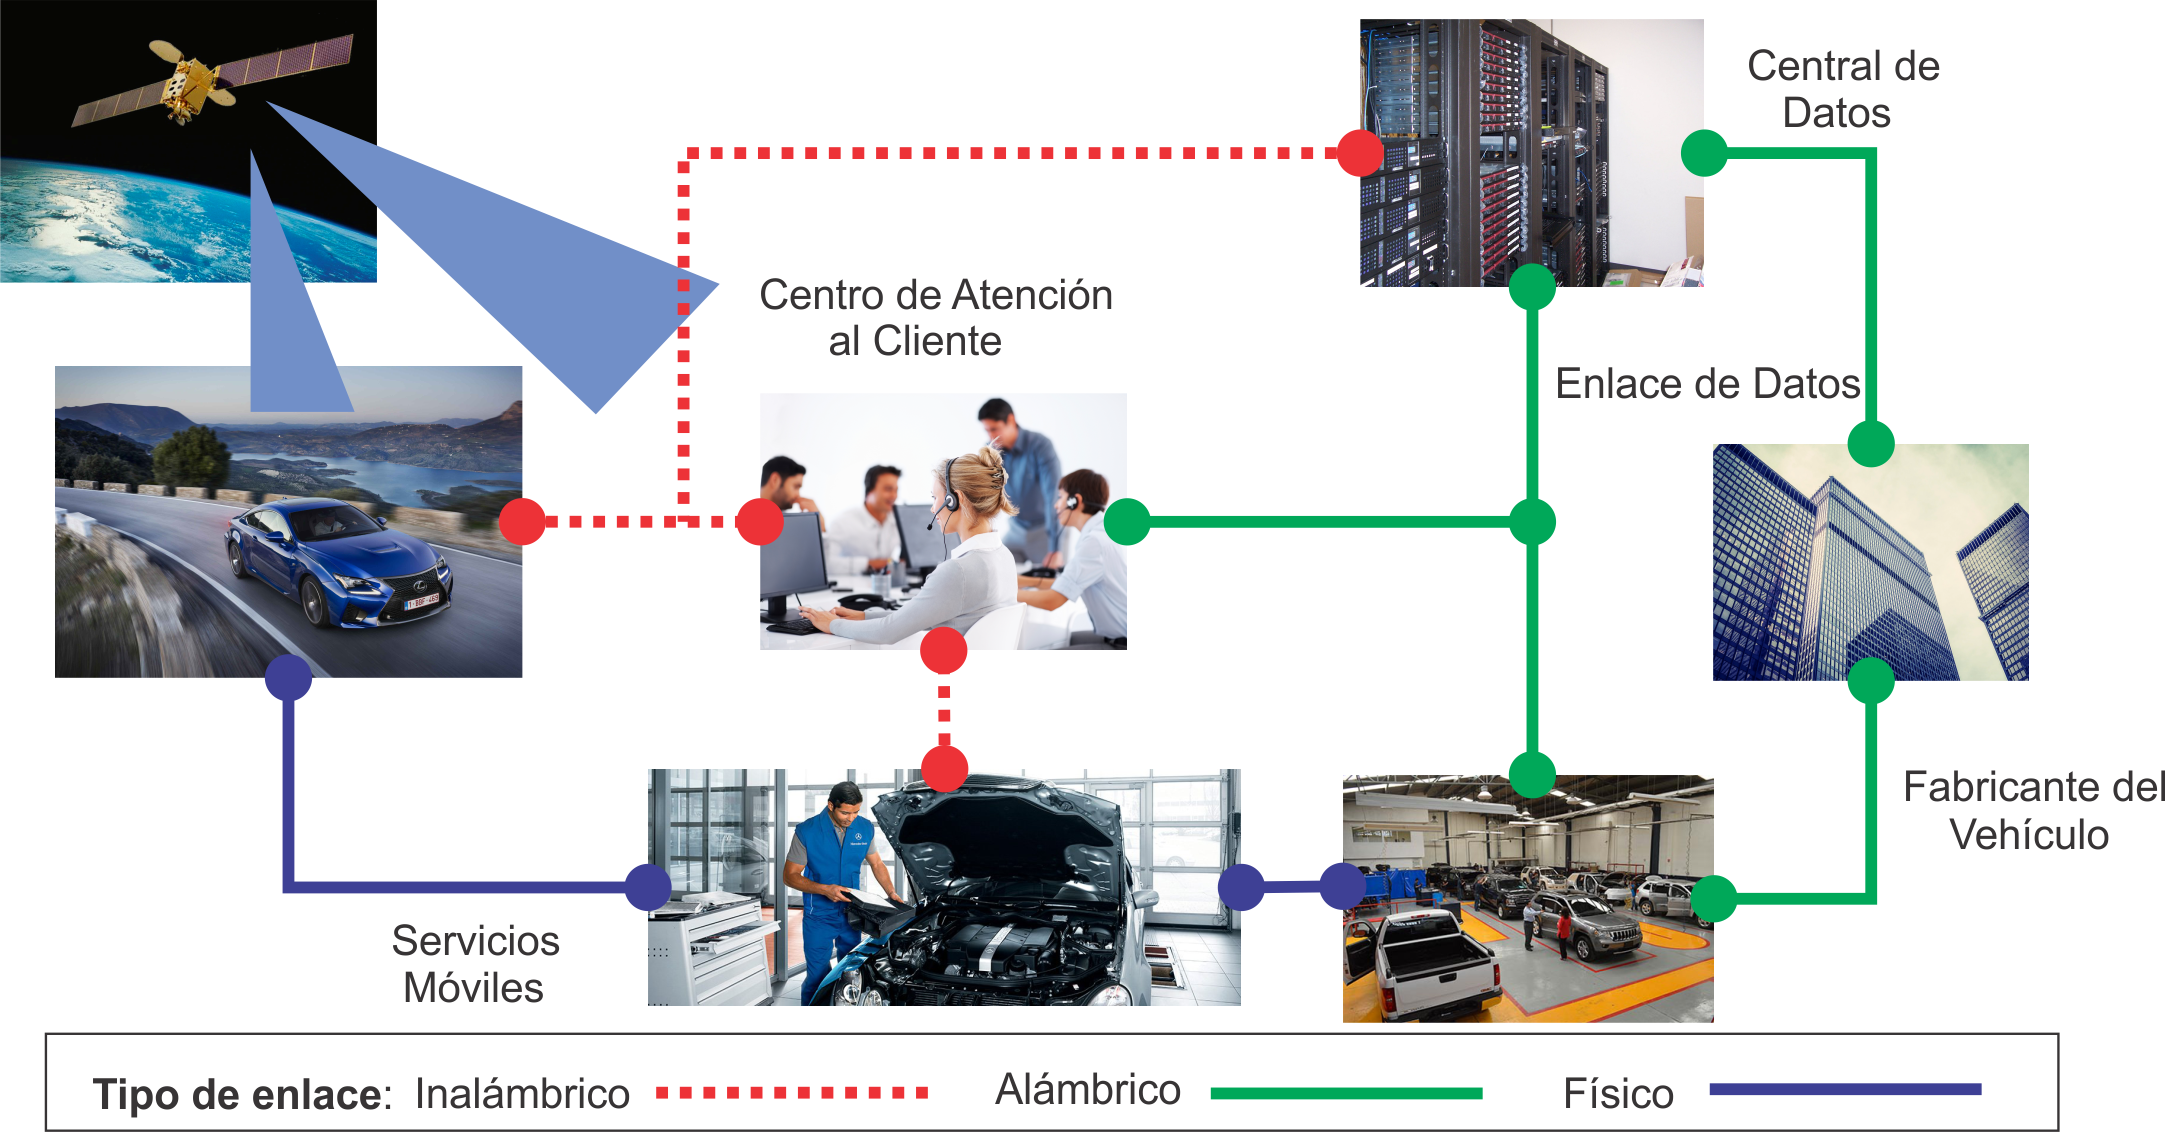
\includegraphics[width=0.8\textwidth]{./Cap2imagen/J_concepto_OBDIII.png}
	\caption[Diagrama de bloques general del concepto OBD-III.]{Diagrama de bloques general del concepto OBD-III.\textbf{ Fuente:} \cite{DE}.}
	\label{DenB} % preguntar que va aquí
\end{figure}


\section {EL Protocolo BUS CAN}

El desarrollo del  protocolo BUS CAN se debió al incremento de los dispositivos electrónicos en los vehículos como por ejemplo el administrador del motor, controlador de luces, aire acondicionado, entre otros.  El desarrollo del protocolo BUS CAN fue necesario para intercambiar de una mejor manera la información entre los diferentes sistemas de control y sus sensores.
Cuando no existía el protocolo BUS CAN los vehículos tenían un sistema de control e intercambio de información mediante conexiones punto a punto, es decir, los modulos que deseaban comunicarse entre si, debían estar conectados de forma directa o indirecta.
En una conexión  directa  cada línea de comunicación está asociada a un par de estaciones o dispositivos, los cuales intercambian información a través de dicha conexión, en cambio, en una conexión indirecta  la comunicación es realizada  mediante una o más estaciones intermediarias.
A medida que las necesidades de control en los vehículos  aumentaron se necesitaban de muchas conexiones y muchas líneas de comunicación, afectando considerablemente el costo de los materiales y el tiempo de producción del vehículo. La solución a este problema es la conexión de los dispositivos y sensores en un bus serial común para todos.

\subsection {Reseña Histórica}
La firma alemana Robert Bosch GmbH inició un proyecto de desarrollo de un protocolo de comunicación entre los distintos dispositivos y sensores  electrónicos para el interior del vehículo en el año 1983. Durante la especificación del sistema de bus serial se unió la empresa fabricante de automóviles Mercedez-Benz y el fabricante de semiconductores Intel Corp. 
Robert Bosch presenta oficialmente el sistema serial BUS CAN en febrero del año 1986, en el congreso de la Sociedad de Ingenieros Automotrices (SAE), celebrado en la ciudad de Detroit, Estados Unidos.
A un año después, la firma Intel realizo la primera implementación física del protocolo en el controlador CAN 82526 y tiempo después la firma Philips introdujo el controlador CAN 82C200, ambos integrados son la base del desarrollo de los controladores actuales.
No tardo mucho para que el protocolo BUS CAN trascendiera a ambientes fuera de lo automovilístico, de hecho las primeras aplicaciones aparecieron en las ramas industriales, como por ejemplo sistemas de control de elevadores, maquinas textiles, maquinas de rayos X entre otros.
Fue en 1992 cuando Mercedez-Benz implementó el protocolo  CAN en sus vehículos Clase "S". El sistema estaba compuesto por dos redes CAN, en la cual una red era de alta velocidad para la comunicación de las ECUs del motor, de la caja de cambios y el tablero de instrumentos; y una red de baja velocidad para el control del aire acondicionado y de los dispositivos electrónicos internos.  Esta implementación de Mercedez-Benz impulso a que otros fabricantes de automóviles comenzaran a utilizar redes BUS CAN en sus modelos de lujo, por ejemplo, BMW, Jaguar, Volvo, Saab, y VW, más tarde se agregaron a la lista Fiat, Renault y PSA. 
La estandarización del protocolo CAN se logro en el año 1993 bajo la norma ISO 11898. Varias versiones y mejoras aparecieron a partir de entonces, \cite{DSEEPC}.

\subsection {Clasificación de las Aplicaciones Automotrices}
La SAE estableció la siguiente clasificación formal de acuerdo a las áreas de aplicación dentro del automóvil:
\begin {itemize} 

\item \textbf{Clase A:} Se refiere a la comunicación con nodos no inteligentes como interruptores, luces, posición del asiento, posición de los espejos, seguros de puertas, etc. La información que se transmite requiere bajas velocidades de transferencia de datos, menor a 10Kbps. La conexión de cables es sencilla y los costos por conexión de nodos es bajo.

\item \textbf {Clase B:} En esta clase se distribuye una mayor cantidad de información, aquí se incluye la actualización del tablero de instrumentos y el control del aire acondicionado. La velocidad de transferencia de datos esta en el orden de 40Kbps

\item \textbf{Clase C:} Comprende la transmisión de datos en tiempo real (real time) con latencia de mensajes menores a 1ms. En esta clase los paquetes de datos transmitidos son mayor a 1 byte a una velocidad que va de 250Kbps a 1Mbps. Dentro de esta categoría están las aplicaciones de comunicación entre los diferentes sistemas de control  de motor, transmisión, estabilidad, frenos y dirección.

\item \textbf{Clase D:} En esta categoría se comunican grandes bloques de datos para aplicaciones de conexión del sistema de radio, teléfono, navegación GPS, consola de interfaz para controladores genéricos que tienen la finalidad de descargar programas, etc. La velocidad de datos requeridas está en el rango de 1 a 10Mbps \cite{DSEEPC}.
\end{itemize}

\section {Características del Protocolo BUS CAN}

El BUS CAN es un protocolo de comunicación serie que soporta control distribuido en tiempo real con un alto nivel de seguridad y multiplicación  \cite{PSMR}. La red de BUS CAN comunica todos los dispositivos a través de un único bus de comunicación de datos, a estos dispositivos se los denomina comúnmente como nodos. Cada nodo es capaz de interactuar con cualquier otro nodo sin la necesidad de una conexión punto a punto entre ellos.
El protocolo BUS CAN está definido internacionalmente por el conjunto de estándares ISO 11898, en dónde se definen las caracteristicas del protocolo, la capa física del bus, sus sistemas para alta y baja velocidad entre otros. El otro estándar que lo acompaña en el proceso de desarrollo del BUS CAN es la ISO 16845, el cual proporciona una  metodología y un conjunto de pruebas necesarias para comprobar la conformidad de cualquier implementación BUS CAN con base a la norma ISO 11898-1 \cite{ISO}, de esta manera se garantiza la comunicación entre los nodos BUS CAN de distintos fabricantes.

\subsection {Capas del Modelo OSI y Capas del Protocolo CAN}
El modelo de comunicación desarrollado por la ISO (International Organization for Standardization, por sus siglas en inglés), llamado OSI (Open System Interconnection, por sus siglas en inglés), es popular debido a que ayuda a dar una explicación  sencilla de la relación entre el hardware  y los protocolos utilizados en una red. El modelo OSI está conformado por 7 capas en las cuales cada una de las capas cumple con una función específica, que permite realizar la comunicación en una red.
La arquitectura del protocolo BUS CAN como muestra en la \textbf{Figura \ref{ABC}}, de acuerdo al modelo de referencia OSI incluye tres capas: Física, Enlace de Datos y Aplicación, además establece una capa especial para la gestión y control del nodo llamada Capa de Supervisor. 


\begin{figure}[H]
	\centering
		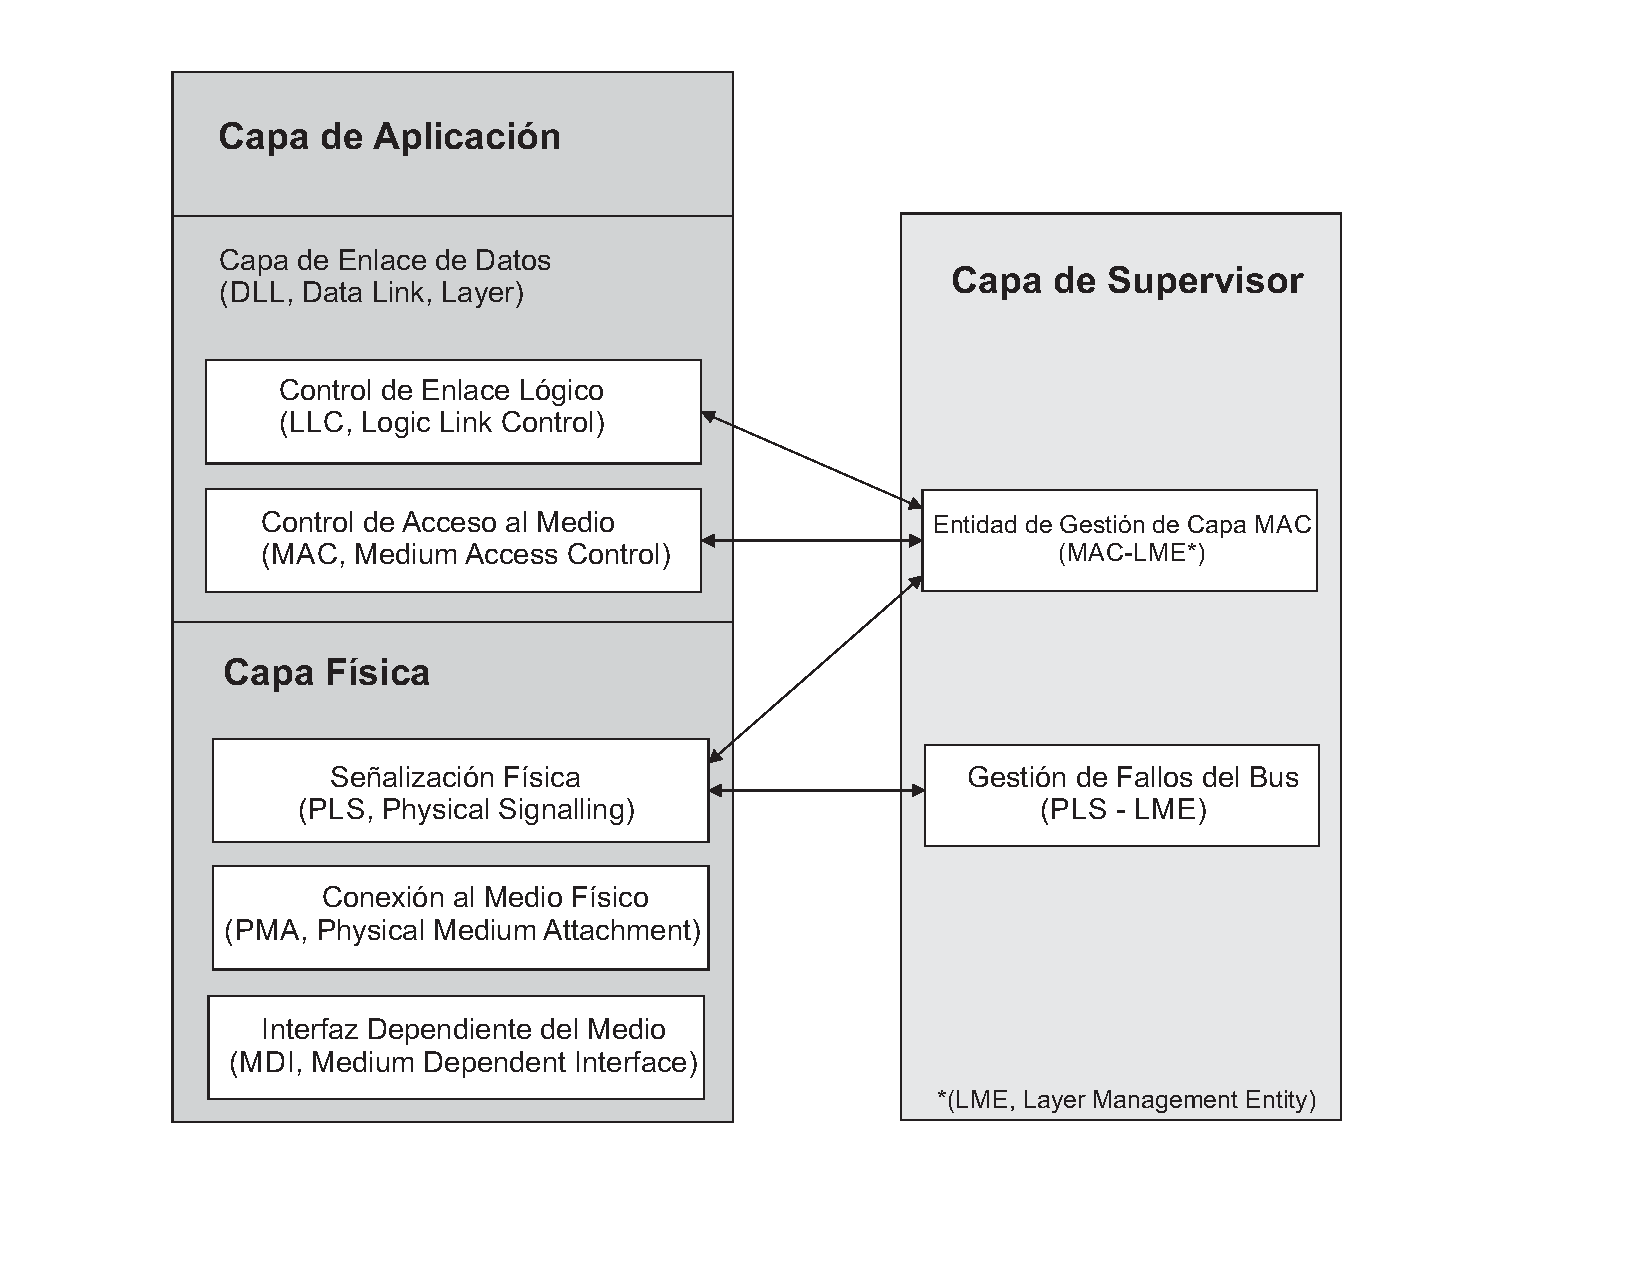
\includegraphics[width=0.8\textwidth]{./Cap2imagen/protocolocan.pdf}
	\caption[Arquitectura de protocolos BUS CAN.]{Arquitectura de protocolos BUS CAN.\textbf{ Fuente:} \cite{DSEEPC}.}
	\label{ABC} % preguntar que va aquí
\end{figure}

\subsubsection  {Capa Física}

La capa física es responsable por la transferencia de bits entre diferentes nodos de red y define los aspectos del medio físico para la transmisión de datos entre los nodos. Los más importantes hacen referencia a los niveles de señal, sincronización, representación y tiempos en que los bits se transfieren al bus. 
Las especificaciones Bosch del protocolo BUS CAN no define una capa física, sin embargo, el estándar  ISO 11898 establece las características que deben cumplir las aplicaciones para la transferencia en alta y baja velocidad.
 
%\subsubsubsection{SubCapa Fisica} %%%%%% lo cambie
\paragraph{SubCapa Física}

La SubCapa de señalización física (PLS, Physical Layer Signalling, por sus siglas en inglés) define la representación, tiempo y sincronización de los bits, y está implementada en los controladores del protocolo BUS CAN.


%\subsubsubsubsection {Representación de los bits}
\paragraph{Representación de los Bits}

Una trama BUS CAN está codificada de acuerdo con el método NRZ (No Return Zero, por sus siglas en inglés), el cual produce una frecuencia de menor operación. Sin embargo, en el caso de transmitir una gran cantidad de bits con la misma polaridad, la codificación NRZ no proporciona flancos que puedan utilizarse en la sincronización y para ello se implementa el procedimiento de inserción de bit (bit-stuffing) \textbf{Figura \ref{IB}}, Asegura que en la transmisión de una trama BUS CAN solamente puede haber un máximo de 5 bits consecutivos con la misma polaridad.



\begin{figure}[H]
	\centering
		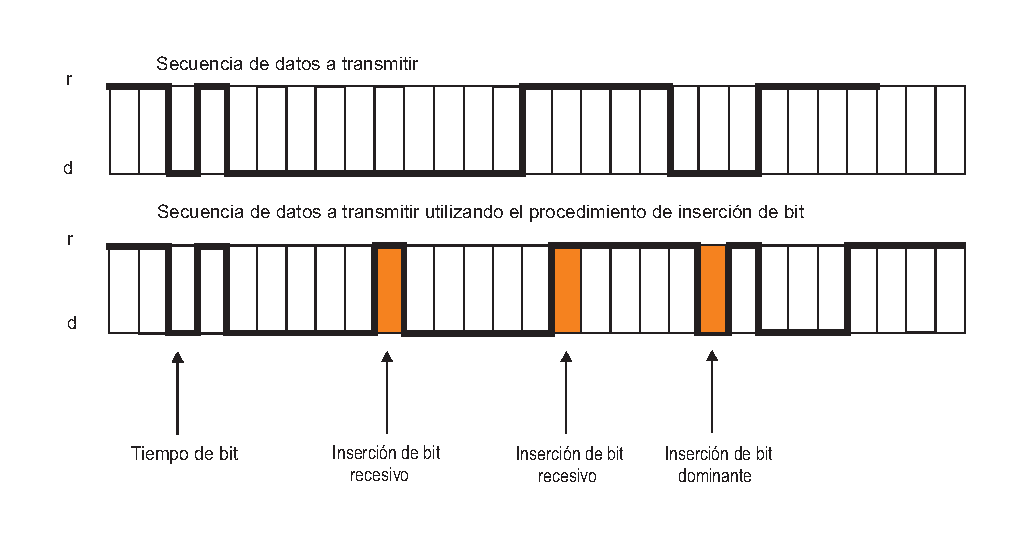
\includegraphics[width=0.8\textwidth]{./Cap2imagen/insercionbit.pdf}
	\caption[Inserción de bit.]{Inserción de bit.\textbf{ Fuente:} \cite{DSEEPC}.}
	\label{IB} % preguntar que va aquí
\end{figure}

%\subsubsubsubsection {Temporización de Bits}
\paragraph{Temporización de Bits}

 El protocolo BUS CAN tiene flexibilidad para determinar los parámetros de velocidad de transferencia, punto de muestreo de bit y número de muestras realizadas en un periodo de bit. Por lo tanto en el diseño de una red BUS CAN se debe tener en cuenta los siguientes conceptos:

\begin{itemize}

\item Tiempo de bit ($t_b$): es el tiempo de duración de un bit.
\item Velocidad de transferencia nominal ($f_b$): es el número de bits por segundo que una transmisión ideal emite sin sincronización.
\item Tiempo de bit nominal: se obtiene mediante la \textbf{Ecuación \ref{eq1}} y se divide en cuatro segmentos de tiempo.

\end{itemize}

La longitud de los segmentos de tiempo en un intervalo de bit está definida en multiples enteros definidas por el periodo de un  oscilador $t_{clk}$. El parámetro $t_q$ es la unidad de tiempo discreta más pequeña utilizada en un modulo BUS CAN. En la \textbf{Figura \ref{TB}} se puede observar los segmentos de tiempo de un bit y en la \textbf{Figura \ref{DB}} se puede observar la derivación del tiempo de un bit.

%insertar ecuacion:::
\begin {equation}
\label {eq1}
t_b = \frac {1}{f_b}
\end {equation}
% insertar ecuacion___

\begin{figure}[H]
	\centering
		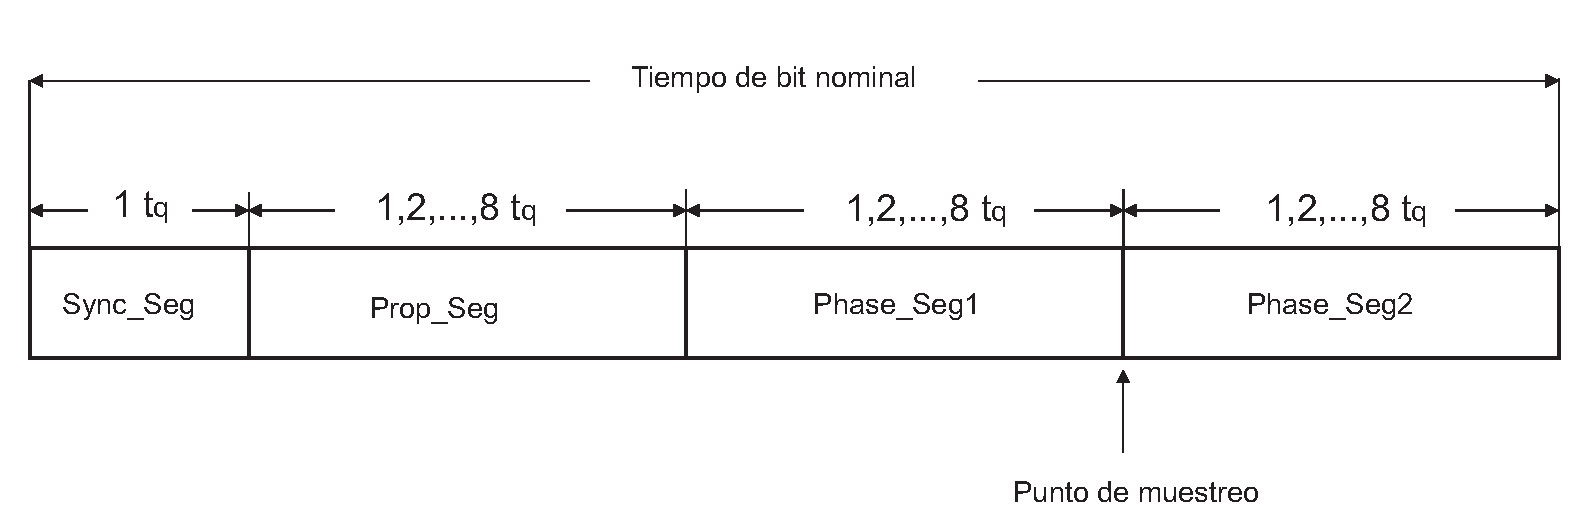
\includegraphics[width=0.8\textwidth]{./Cap2imagen/tiempo_bit.pdf}
	\caption[Segmento del tiempo de un bit.]{Segmento del tiempo de un bit.\textbf{ Fuente:} \cite{DSEEPC}.}
	\label{TB} % preguntar que va aquí
\end{figure}

\begin{figure}[H]
	\centering
		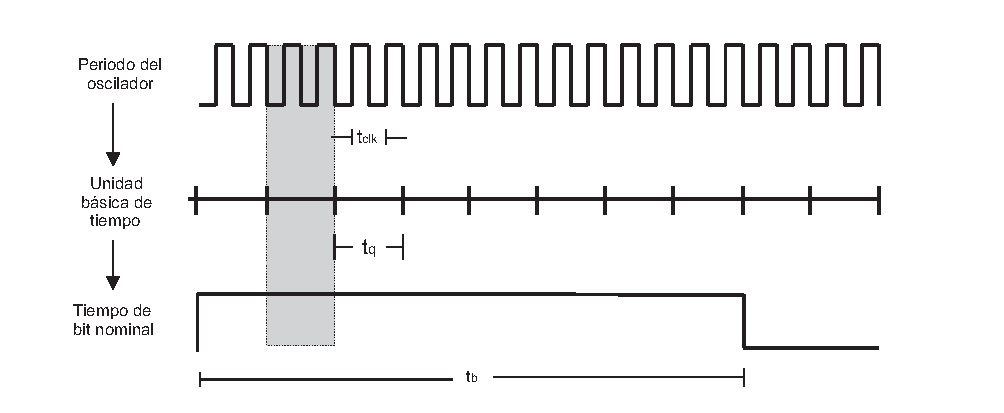
\includegraphics[width=0.8\textwidth]{./Cap2imagen/derivacion_bit.pdf}
	\caption[Derivación del tiempo de un bit.]{Derivación del tiempo de un bit.\textbf{ Fuente:} \cite{DSEEPC}.}
	\label{DB} % preguntar que va aquí
\end{figure}


Los cuatro segmentos que forman un tiempo de bit nominal son:

\begin{itemize} % para crear una lista
\item Segmento de sincronización (Sync Seg): se utiliza para sincronizar los diferentes nodos del bus en un flanco dentro del mismo segmento.
\item Segmento de tiempo de propagación (Prog Seg): sirve para compensar los tiempos de retardos físicos originados por la propagación de la señal en el bus y por los retardos internos en los nodos.
\item Segmento de memoria temporal de fase 1 (Phase Seg1): se utiliza para compensar variaciones de tiempo entre los nodos y puede incrementarse durante la resincronización.
\item Segmento de memoria temporal de fase 2 (Phase seg2): se utiliza para compensar variaciones de tiempo entre los nodos y puede reducirse durante la resincronización.

\item Punto de muestreo (sample point): instante del tiempo en que se lee e interpreta el nivel del bus y se proporciona el valor del bit respectivo.
\item Tiempo de procesamiento de la información: Es el periodo de tiempo que comienza con el punto de muestreo y se utiliza para calcular el nivel de bit subsecuente.
\end{itemize}

Para la transferencia de bits entre distintos nodos de red es necesario estudiar la capa física, la cual define parámetros como los niveles de señal, la sincronización, la impedancia de la línea de bus de comunicación de acuerdo con el medio físico adoptado y la velocidad de comunicación entre ellos. En el protocolo BUS CAN no todos los nodos conectados a la red mediante el bus necesitan transmitir a la misma velocidad, esto dependerá de las funciones que desempeña cada nodo y de la importancia de sus mensajes, es por ello que el protocolo BUS CAN posee varias tasas de transmisión de bits especificados  por el estándar ISO. Las velocidades van desde la tasa baja de 125kbps hasta la tasa alta de 1Mbps.
La capa física define el medio de transmisión. La representación de los niveles lógicos en las líneas del bus de comunicación BUS CAN es realizada de acuerdo al nivel de tensión que serán establecidos en el mismo bus. Existen dos variables para representar las líneas del BUS: CANH y CANL. Un bit recesivo (1 lógico) es representado a través de dos líneas del bus con un nivel de tensión de 2.5V, de modo que la diferencia de potencial entre CANH  y CANL será de 0V, en cambio, un bit dominante (0 lógico) es representado colocando el CANH = 3.5V y el CANL = 1.5V. Esto da una diferencia de potencial para un bit dominante de cerca de 2V, \cite{PSMR}. De esta manera los datos no son representados por bits de nivel “0” y “1”, sino son representados por bits dominantes y recesivos como se muestra en la \textbf{Figura \ref{N_N}} . 


\begin{figure}[H]
	\centering
		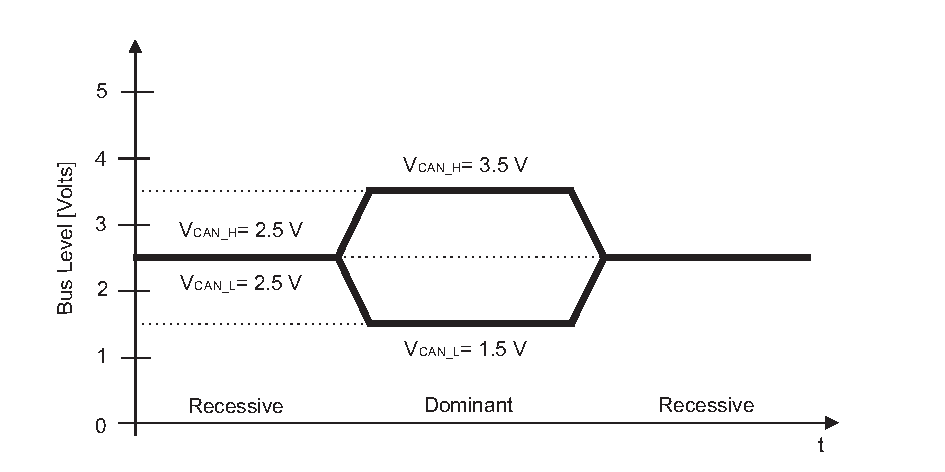
\includegraphics[width=0.8\textwidth]{./Cap2imagen/niveles.pdf}
	\caption[Niveles nominales de la señal BUS CAN ISO 11898.]{Niveles nominales de la señal BUS CAN ISO11898.\textbf{ Fuente:} \cite{PSMR}.}
	\label{N_N} % preguntar que va aquí
\end{figure}

Para evitar que los datos sean reflejados en forma de eco en el BUS de comunicación se colocan en los extremos del BUS, entre CANH y CANL, unas resistencias cuyos valores son empíricos, como se muestra en la \textbf{Figura \ref{T_B}}. 


\begin{figure}[H]
	\centering
		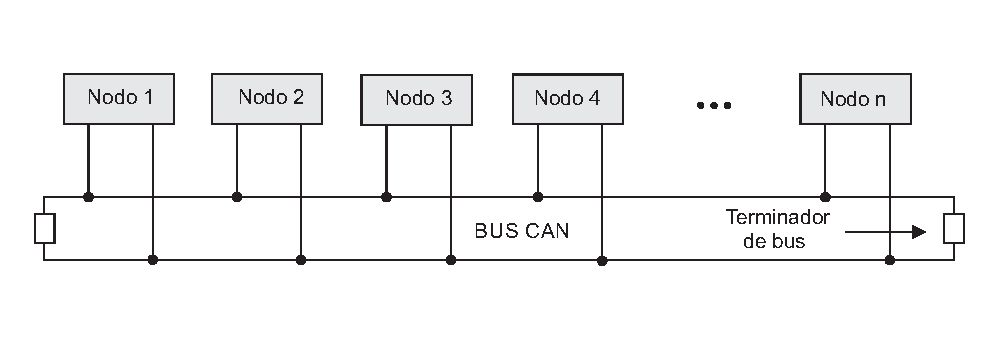
\includegraphics[width=0.8\textwidth]{./Cap2imagen/terminador.pdf}
	\caption[Terminador de bus.]{Terminador de bus.\textbf{ Fuente:} \cite{PSMR}.}
	\label{T_B} % preguntar que va aquí
\end{figure}


\subsubsection {Capa de Enlace de Datos}
%%%% desde aqui
Esta capa describe el método para el intercambio de datos entre nodos dentro de un medio común.
Los mensajes transmitidos por la red BUS CAN tiene dos versiones: la 2.0A y la 2.0B, en la primera un campo de la trama, destinado para el identificador,  está formada por 11 bits mientras que en la segunda está formada por 29bits.
En la capa de enlace para el protocolo BUS CAN se utilizan dos subcapas: MAC (Media Access Control) y LLC (Logical Link Control).

\subsubsection {MAC}

En la red BUS CAN se brinda procesamiento en tiempo real a todos los nodos conectados al bus.  Para que los nodos tengan acceso al medio se utiliza un mecanismo de arbitraje que se describe a continuación:

\begin{itemize}
\item Cuando un nodo intenta acceder al medio y comunicarse con otro nodo, la capa de aplicación realiza la petición para envío de trama. En esta situación puede ocurrir que la capa de aplicación de varios nodos inicien el mismo procedimiento simultáneamente. Esto en el protocolo BUS CAN se resuelve asignando prioridades mediante el ID (identificador) de cada mensaje \textbf{Figura \ref{LID}}. Esto se realiza en el diseño del sistema, no puede modificarse de forma dinámica. El ID con menor número binario es el que posee mayor prioridad.
\item Para acceder al medio se utiliza el CSMA/CD+AMP (Carrier Sense Multiple Access/Collision Detection with Arbitration on Message Priority, por sus siglas en inglés). Esto hace que los nodos que desean transmitir un mensaje en la red deban esperar a que el bus este libre, cuando esto pasa los nodos transmiten un bit de inicio (acceso multiple). Cada nodo lee el bus durante la transmisión y compara bit a bit la trama transmitida con la recibida, si se detecta una diferencia se lleva a cabo un mecanismo de arbitraje.

\end {itemize}

\begin{figure}[H]
	\centering
		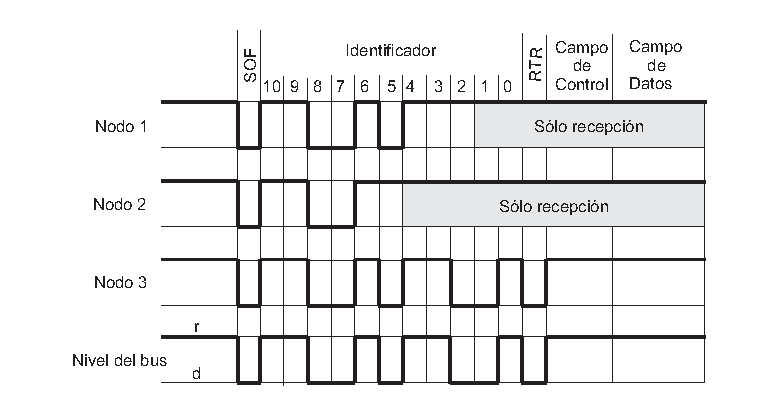
\includegraphics[width=0.8\textwidth]{./Cap2imagen/logicacan.pdf}
	\caption[Lógica del BUS CAN.]{Lógica del BUS CAN.\textbf{ Fuente:} \cite{PSMR}.}
	\label{LID} % preguntar que va aquí
\end{figure}


\subsubsection {LLC}
Es la capa del enlace de datos cuyas funciones son:

\begin {itemize}
\item Filtrar mensajes: El ID no define la dirección de destino del mensaje pero si el contenido, cada receptor recibe el mensaje y el mismo receptor determina si es para él o no.
\item Notificar sobrecarga: si las condiciones internas del receptor requieren un retraso en la transmisión del mensaje, la sub capa LLC transmite una notificación de sobre carga.
\item Proceso de recuperación: La sub capa LLC da la posibilidad de retransmisión automática de tramas cuando pierde su arbitraje o presenta un error en la transmisión.
\end{itemize}

\subsubsection {Transmisión de Mensajes}
Para la transmisión y control de mensajes se define cuatro tipos de tramas: la trama de datos, la trama remota , la trama de error y la trama de sobre carga.

\begin{itemize} % ITEM PRINCIPAL
\item Trama de datos:  la trama de datos está formada por 7 campos, \textbf{Figura: \ref{TRD}}.

			\begin{figure}[H]
			\centering
				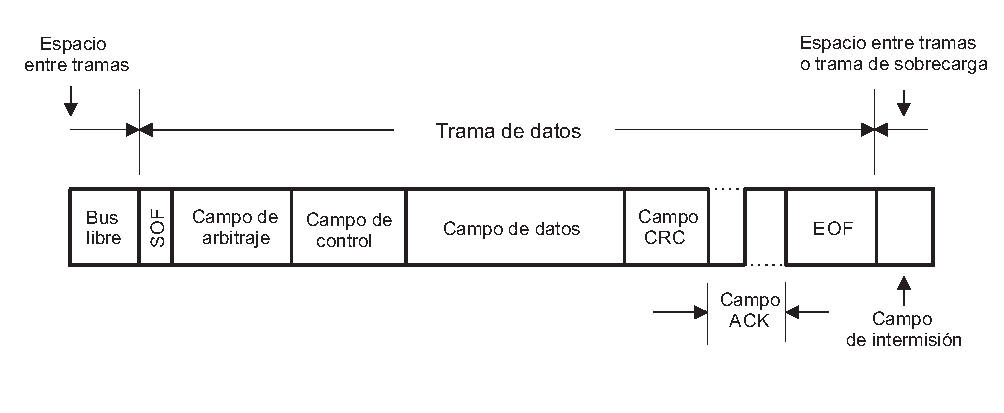
\includegraphics[width=0.9\textwidth]{./Cap2imagen/trama_datos.pdf}
			\caption[Formato de la trama de datos.]{Formato de la trama de datos.\textbf{ Fuente:} \cite{PSMR}.}
			\label{TRD} 
			\end{figure}

				\begin{itemize} %ITEM SECUNDARIO%4tabulaciones
				\item SoF (Stad of Frame): determina el inicio de la trama de datos y consiste en un bit dominante que sincroniza a todos los nodos activos en la red. Es el mismo para la trama estándar y extendida del BUS CAN.
				\item Arbitration field: este campo cambia de acuerdo al formato de la trama.
										
											\begin {itemize} %ITEM TERCIARIO%8tabulaciones
											\item El formato estándar está formado por un identificador de $11$ bits  y el bit de petición de transmisión remota RTR (Remote Transmission Request, por sus siglas en inglés). El bit menos significativo del identificador se transmite al último, además, no pueden ser recesivos los 7 bits más significativos.
											\item En el formato extendido la trama tiene un identificador de $29$ bits, el bit de petición substituta SRR(Sustitute Remote Request, por sus siglas en inglés), el bit de extensión del identificador IDE(Identifier Extension) y el bit RTR. El identificador se divide en dos secciones: la primera denominada base (base ID) que es de $11$bits y la segunda sección de 18 bits conocida como extendida (extended ID). Los bits se transmiten en orden de mayor a menor prioridad.
											\end {itemize} % FIN DE TERCIARIO

El bit RTR debe ser dominante para ambos formatos de trama de datos y el bit SRR es un bit recesivo, por lo tanto las posibles colisiones entre ambos tipos de formatos de trama que tengan el mismo valor en el campo Base ID se resuelven de manera que el formato de trama estándar predomina sobre el formato de trama extendida. En dicha resolución también se involucra el bit IDE, el cual pertenece al campo de arbitraje en el caso de un formato extendido y se encuentra en el campo de control para el caso de un formato de trama estándar. La transmisión del bit IDE es dominante para el formato estándar y recesivo para el extendido. En la \textbf{Figura: \ref{FEE}} se especifica la diferencia entre el formanto estándar y el formato extendido

			\begin{figure}[H]
			\centering
				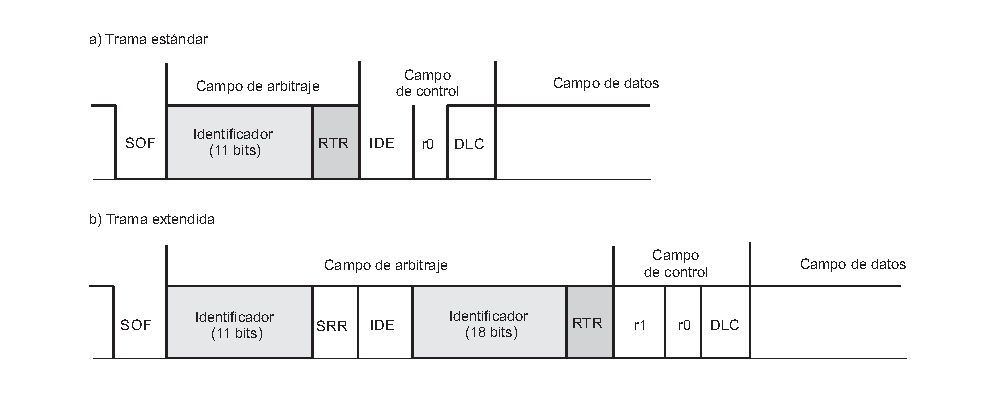
\includegraphics[width=0.9\textwidth]{./Cap2imagen/datos_est_ext.pdf}
			\caption[Trama de datos estándar y extendido.]{Trama de datos estándar y extendido.\textbf{ Fuente:} \cite{PSMR}.}
			\label{FEE} 
			\end{figure}


				
				
				\item Control Field: Está compuesto de seis bits, IDE/r$1$, r$0$ y cuatro bits que forman el código de longitud de datos DLC (Data Length Code, por sus siglas en inglés). El primer bit que se transmite es IDE, el cual distingue entre los dos tipos de tramas; seguida r$0$, en nivel dominante y está reservado para futuras aplicaciones del protocolo BUS CAN; finalmente se transmite el DLC para indicar el numero de octetos contenidos en el campo de datos. 
				\item Data Field: Puede tener una longitud de $0$ a $8$ octetos y contiene el mensaje a transmitir en la trama de BUS CAN. EL bit con mayor prioridad se transfiere primero.
				\item CRC (Cyclic Redundant Check, por sus siglas en inglés): Es una secuencia de $15$ bits de verificación y un bit delimitador CRC (CRC delimiter) transmitido en un nivel recesivo. Mediante este campo se verifica si la trama fue alterada.
				\item ACK (Acknowledgement, por sus siglas en inglés): está formada por dos bits : ACK (ACK slot) y delimitador ACK (ACK delimiter), este último siempre se transmite en un nivel recesivo. Todo nodo activo en la red CAN que recibe una trama válida, sobrescribe la ranura ACK con un nivel dominante, y con ello el transmisor verifica que su mensaje se envió correctamente. si por el contrario ningún nodo sobrescribe dicha ranura, el transmisor considera un error de transmisión.
				\item End of Frame: El fin de la trama de datos y la trama remota están delimitadas por una secuencia de 7 bits recesivos que indican el fin de la trama. Cuando el EOF está activo se realiza una violación al procedimiento de inserción de bit, por ello dicho procedimiento no se aplica a este campo.
				\end{itemize} %FIN SECUNDARIO



\item Trama remota: permite iniciar una transmisión de mensaje de un nodo estando este en modo recepción mediante el envío de esta trama. Los campos de una trama remota son los mismos que la de una trama de datos, a excepción que la trama remota no contiene el campo de datos y el bit RTR es recesivo. EL valor del DLC debe coincidir con el de la trama de datos correspondiente. En la \textbf{Figura: \ref{TR}} se exponen las características de la trama.

			\begin{figure}[H]
			\centering
				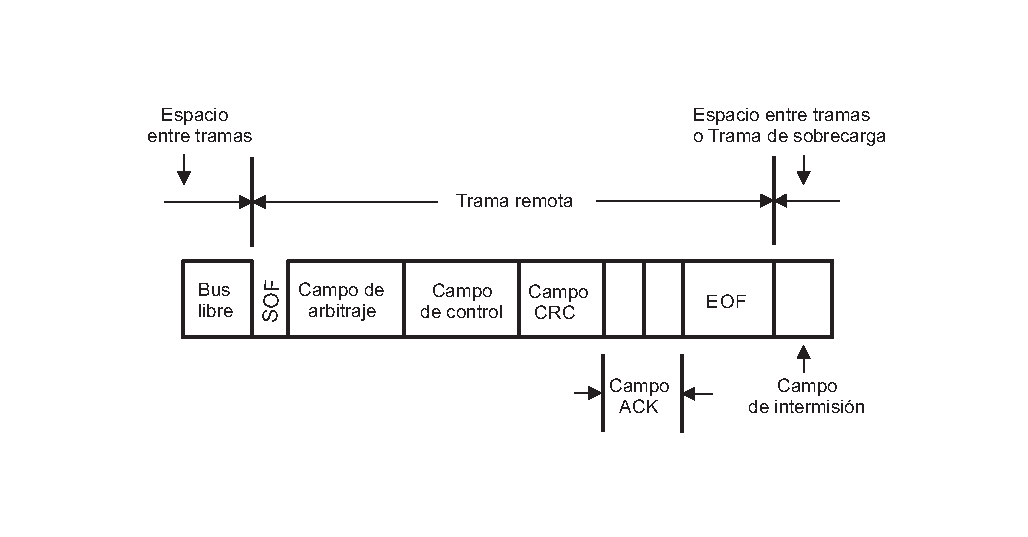
\includegraphics[width=0.9\textwidth]{./Cap2imagen/tramaremota.pdf}
			\caption[Formato de trama remota.]{Formato de trama remota.\textbf{ Fuente:} \cite{DSEEPC}.}
			\label{TR} 
			\end{figure}


\item Trama de error: durante la transmisión o recepción de una trama de datos o una trama remota, esta trama señaliza la detección de un error, iniciando nuevamente el envió del mensaje. En la \textbf{Figura: \ref{TE}} se expone como la trama de error está formada por dos campos:

							\begin{itemize}
							\item Error flag: hay dos formas de representarla:
										\begin {itemize}
										\item Active error flag: son seis bits dominantes consecutivos.
										\item Passive error flag: son seis bits recesivos consecutivos, pero pueden sobrescribirse con bits dominantes de otros nodos.
										\end {itemize}
							\item Error delimiter: una trama de error termina con una secuencia de $8$ bits recesivos. Posterior a la transmisión de una bandera de error, el nodo transmite bits recesivos y verifica el nivel del bus hasta que reconozca un bit recesivo, entonces comienza la transmisión de otros siete bits recesivos. Con este mecanismo, el nodo puede determinar si fue el primero en transmitir una bandera de error y con ello detectar una condición de error.
							\end {itemize}
							
								\begin{figure}[H]
								\centering
								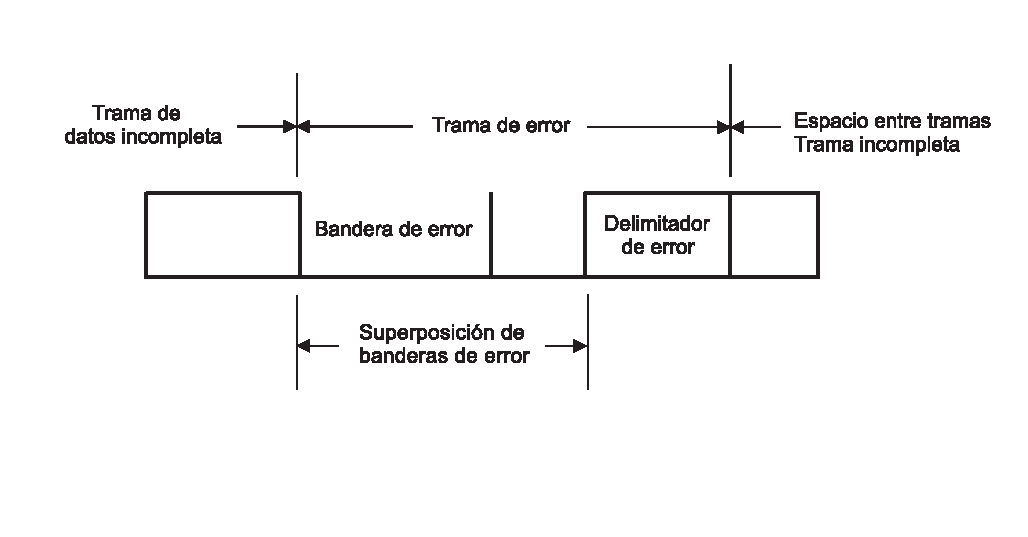
\includegraphics[width=0.9\textwidth]{./Cap2imagen/trama_error.pdf}
								\caption[Formato de trama de error.]{Formato de trama de error.\textbf{ Fuente:} \cite{DSEEPC}.}
								\label{TE} 
								\end{figure}


					
\item Trama de sobre carga: un receptor puede solicitar un retraso en la transmisión de la siguiente trama si las condiciones internas del receptor requieren un retraso en la transmisión del mensaje. Se permite en el protocolo BUS CAN el envio de dos tramas de sobre  carga como máximo, \textbf{Figura: \ref{TSC}}.
Las tramas de sobrecarga se transmiten después de detectar las siguientes condiciones de error: 


					\begin{itemize}
		
					\item Detección de un bit dominante durante los primeros dos bits del campo de intermisión. La detección de un bit dominante en el tercer bit del campo de intermisión se interpreta como un SOF. 
					\item Cuando un receptor detecta un bit dominante en el ultimo bit del campo EOF, o cuando un nodo receptor o transmisor detecta un bit dominante en el ultimo bit del delimitador de una trama de error o sobrecarga.
					\end{itemize}

Una trama de sobrecarga se considera una forma especial de trama de error y tiene los siguientes campos:
	
								\begin{itemize}
								\item Overload flag: se constituye por ocho bits dominantes. La forma completa corresponde a la bandera de error activa.
								\item Oveload delimiter: formado por 8 bits recesivos.
								\end{itemize}


			\begin{figure}[H]
			\centering
				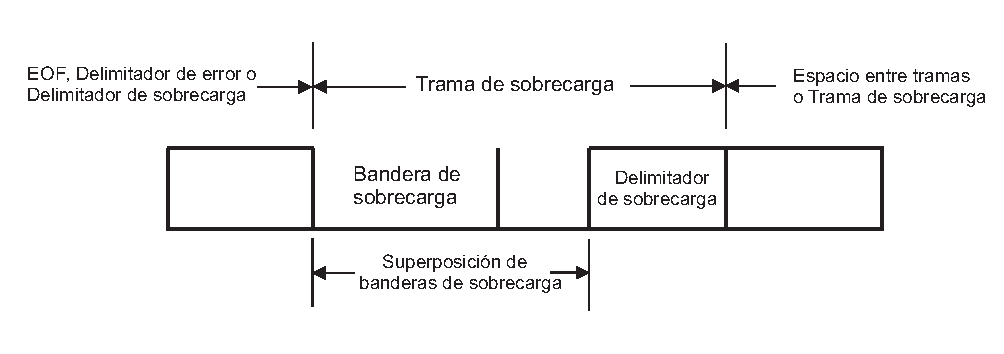
\includegraphics[width=0.9\textwidth]{./Cap2imagen/sobrecarga.pdf}
			\caption[Formato de trama de sobrecarga.]{Formato de trama de sobrecarga.\textbf{ Fuente:} \cite{DSEEPC}.}
			\label{TSC} 
			\end{figure}
				
\end{itemize}

\subsubsection {Espacio Entre Tramas}

Para tener en cuenta las tramas de datos y las tramas remotas están separadas por un espacio entre tramas, en cambio las tramas de error y las tramas de sobrecarga se transmiten en forma sucesiva.
Además el espacio entre tramas está formado por tres campos:

	\begin{itemize}
	\item Intermission: Consiste en tres bits recesivos. Durante su transmisión la única acción que puede realizarse es señalar una condición de sobrecarga, y no se permite que ningún nodo inicie la transmisión de una trama de datos o remota. 
	\item Bus Idle: Se mantiene un nivel recesivo hasta que un nodo inicie la transmisión de una trama nueva.
	\item Suspend transmission: El espacio entre tramas contiene un tiempo de inhibición de transmisión de ocho bits para nodos que se encuentran en estado de error pasivo.
	\end{itemize}


%\subsubsubsubsection {Codificación de Tramas}
\paragraph{Codificación de Tramas}

Los campos de inicio de trama, identificador, control, datos y CRC están codificados de acuerdo al procedimiento de inserción de bit. Los campos restantes como el delimitador CRC, ACK y EOF tienen un formato fijo y no siguen el procedimiento de inserción de bit, de igual forma, las tramas de error y sobrecarga tienen un formato fijo y no se codifican por dicho procedimiento.

%\subsubsubsubsection {Validación de Tramas}
\paragraph{Validación de Tramas}

Para validar un trama difiere según el:

\begin {itemize}
\item Transmisor: La trama es válida si no existen errores hasta el final del campo EOF. Si existe un error, en la trama se activa el proceso de recuperación.
\item Receptor: la trama es válida si no existen errores hasta el siguiente bit después del campo EOF.
\end{itemize}


%\subsubsubsubsection {Detección y Manejo de Errores}
\paragraph{Detección y Manejo de Errores}

En una red el controlador de BUS CAN tiene la capacidad de detectar y manejar errores que surjan en la comunicación. Si un nodo detecta un error inmediatamente lo comunica al resto de  los nodos de la red. Si algún nodo lanza errores continuamente el protocolo BUS CAN tiene un algoritmo que se basa en la actividad del bus para desconectar a los nodos que envían fallos permanentemente, de esta manera los demás nodos no son perturbados por estos nodos defectuosos.

%\subsubsubsubsection {Mecanismo de Detección de Errores}
\paragraph{Mecanismo de Detección de Errores}

Para mantener la seguridad de la transmisión de datos, el protocolo BUS CAN define los siguientes mecanismos para la detección de errores: 
\begin{itemize}
\item Monitoreo de bits: Todo nodo verifica que el nivel de bits transmitido sea el mismo nivel del bus, y cuando dichos valores difieren se detecta un bit de error. El monitoreo de bits representa un mecanismo de seguridad global para la detección de todos los errores efectivos.
\item Verificación del procedimiento de inserción de bit: hace referencia al hecho de detectar un error de inserción de bit cuando ocurren seis niveles consecutivos de bits con el mismo valor en un campo de trama codificado por el procedimiento de inserción de bit (Stuff error).
\item Verificación de redundancia cíclica de 15 bits: Se detecta un error de CRC cuando la secuencia de CRC calculada por el nodo no corresponde al campo CRC de la trama recibida.
\item Verificación de trama: Cuando un campo fijo contiene uno o más bits no válidos se detecta un error. 
\item Verificación de aceptación: un transmisor detecta un error de aceptación (ACK error) cuando el slot ACK no cambia de estado dominante.
\end{itemize}


%\subsubsubsubsection {Manejo de Errores}
\paragraph*{Manejo de Errores}

Cuando un nodo detecta algún tipo de error, ya sea de bit, de inserción, de forma o de aceptación, inicia una transmisión de un error flag en el siguiente bit. Cuando se detecta un error de CRC, se inicia la transmisión de una trama de error después del delimitador ACK, a excepción de que previamente se haya transmitido otra trama de error.
El manejo de errores se lleva acabo de acuerdo con el diagrama de flujo de la \textbf {Figura: \ref{D_F}}
%width = 0.33
\begin{figure}[H]
	\centering
		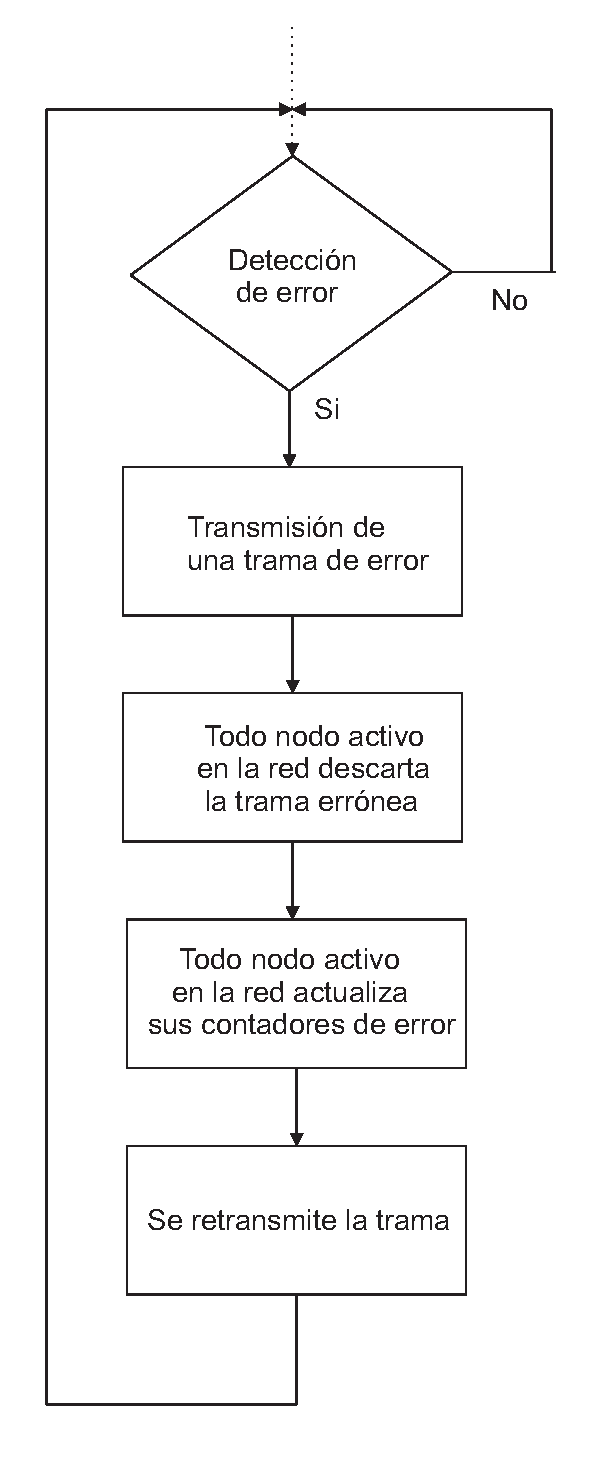
\includegraphics[width=0.40\textwidth]{./Cap2imagen/diagrama.pdf}
	\caption[Diagrama de flujo para manejar errores.]{Diagrama de flujo para manejar errores.\textbf{ Fuente:} \cite{DSEEPC}.}
	\label{D_F} % preguntar que va aquí
\end{figure}

%\subsubsubsubsection {Capacidad de Detección de Errores}
\paragraph{Capacidad de Detección de Errores}

Se utilizan diferentes mecanismos para detectar errores en los protocolos de bus seriales, generalmente se encarga el receptor de esta verificación. La capacidad de detectar errores de transmisión depende de los mecanismos de error y del protocolo utilizado.




\subsubsection {Capa de Aplicación}

La capa de Aplicación no se encuentra especificada en el estándar, por lo que se deja al usuario en la libertad de desarrollarla.
Existen varias aplicaciones utilizadas como por ejemplo CANopen, DeviceNet y CAN aerospace. 

Para utilizar una red BUS CAN de dos lineas, es recomendable utilizar el par trenzado para establecer la comunicación entre estos, debido a que este tipo de cable atenúa los efectos causados por interferencias electromagnéticas. 
La velocidad en una red  BUS CAN es inversamente proporcional a la longitud del bus de comunicación. La mayor tasa de bits especificada es de 1Mbps a una distancia entre nodos de 40m. 

\subsection {Hardware BUS CAN}

\subsubsection{Transceiver}

El Transceiver se encarga de adaptar las señales de un controlador CAN  a los niveles utilizados por el nivel físico. Actúa como transmisor y receptor de datos. Transforma los datos utilizados por el controlador BUS CAN en señales eléctricas que son compatibles con las características eléctricas del bus de comunicación. De la misma manera, este recibe los datos del bus de comunicación y los adapta para que pueda ser recibida por el controlador BUS CAN.

\subsubsection {Controlador BUS CAN}

Encargado de la comunicación entre el microprocesador de la unidad de control y el transceiver. 
 
\subsection{Estandares Existentes}

%Estandares <<
Para entender los estándares presentes en el mercado del protocolo BUS CAN se deben comprender el trabajo de las siguientes sociedades:

\textbf{ SAE Internacional (SAE - Society of Automotive Engineers)}: La Sociedad de Ingenieros Automoción, es la organización enfocada en la movilidad de los profesionales en la ingeniería aeroespacial, automoción, y todas las industrias comerciales especializadas en la construcción de los vehículos. El principal objetivo de la sociedad es el desarrollo de los estándares para todos los tipos de vehículos, incluyendo coches, camiones, barcos, aviones, etc. Cada uno que se interese por los factores humanos y los estándares ergonómicos, puede ser miembro de esta organización. 

Entre uno de los estándares encontramos al OBD-II, todos los vehículos modernos están equipados con el sistema diagnóstico conocido como On-Board Diagnostics II (OBDII, por sus siglas en inglés). Si este funciona mal, la luz de control del motor se enciende para avisar al conductor que tiene que revisar los códigos DTC (Diagnostic TRouble Codes):

SAE se encarga de la estandarización de los datos que se utilizan en el protocolo BUS CAN y en otros protocolos de comunicación en vehículos de automoción, es decir, para los automóviles terrestres estandariza el sistema de diagnóstico conocido como OBD II.

Los estándares SAE más conocidos son: 

\textbf{SAE J1962}: Define las características del conector OBD II.  La especificación prevé dos interfaces de hardware estándar, llamado conector tipo A y conector tipo B, de 16 pines. Ambos tipos tienen una ranura entre las dos filas de pines, pero el tipo B tiene la ranura interrumpida en el medio, \cite{J1962}. 

\textbf{SAE J1979}: Define un método para la solicitud de varios datos de diagnóstico y una lista de parámetros estándar que podrían estar disponibles a partir de la ECU (engine control unit, por sus siglas en inglés), \cite{J1979}.

\textbf{SAE J1850}: Define el tipo de protocolo para el conector OBD II, no necesariamente es BUS CAN. 

\textbf{SAE J2284}: A partir del 2008 este estándar reemplaza al estándar SAE-J1850, define la versión específica de BUS CAN usado en el conector OBD II, \cite{J2284}. 

\textbf{SAE J1939}: Basado en el CAN 2.0B es una capa superior del protocolo CAN para camiones y autobuses que define la SAE, se divide en varias partes que describen la capa física, la capa de enlace de datos, gestión de la red y posee un gran número de mensajes predefinidos, \cite{J1939}, \cite{J1939_}.

\textbf{ISO (International Organization for Standardization)}:  La Organización Internacional de Normalización es el organismo encargado de promover el desarrollo de normas internacionales de fabricación (tanto de productos como de servicios), comercio y comunicación para todas las ramas industriales. Su función principal es la de buscar la estandarización de normas de productos y seguridad para las empresas u organizaciones (públicas o privadas) a nivel internacional, \cite{ISO}.

Actualmente el Protocolo BUS CAN está estandarizado por la ISO según las siguientes normas:

\textbf{ISO 11898-1}: Define el protocolo CAN. Especifica la capa de enlace de datos (DLL) y la señalización física de la red BUS CAN,  de manera a  obtener un protocolo de comunicación serie que soporte el control en tiempo real y la multiplexación para uso dentro de los vehículos de carretera. Contiene especificación detallada de la subcapa  de control de enlace lógico (LLC) y la subcapa de control de acceso al medio (MAC), \cite{ISO1}.

\textbf{ISO 11898-2}: Define la capa física de alta velocidad para BUS CAN. Especifica las características de alta velocidad de la Unidad de Acceso al Medio (MAU, por sus siglas en inglés), y algunas de las características de la Interfaz Dependiente del Medio (MDI, por sus siglas en inglés), que comprenden la capa física de la red de área del controlador BUS CAN, \cite{ISO2}.

\textbf{ISO 11898-3}: Define la capa física de baja velocidad tolerante a fallos para CAN. Especifica las características de la creación de un intercambio de información digital entre las ECU de vehículos equipados con la red de área de controlador BUS CAN a velocidades de transmisión superiores a 40 Kbps hasta 125 Kbps, \cite{ISO3}.

\textbf{ISO 11898-4}: Especifica la comunicación Time-Triggered en el BUS CAN, el cual se basa en el desarrollo de un tipo de intercambio de información de las ECU en los vehículos, \cite{ISO4}.

\textbf{ISO 11898-5}: Describe las funciones de la unidad acceso al medio de alta velocidad (hasta 1Mbps)  en modo bajo consumo mientras no haya comunicaciòn en el bus, \cite{ISO5}. 

\textbf{ISO 11898-6}: Define la unidad acceso al medio de alta velocidad con funcionalidad de atención selectiva.  Representa una extensión de la norma ISO 11898 e ISO 11898-2 al  5, que especifica un mecanismo de atención selectiva utilizando tramas CAN configurables, \cite{ISO6}.

\textbf{ISO 16845}: Establece un plan  y los requisitos de pruebas para verificar si el transceptor BUS CAN con sus distintas funciones está conforme  a las funcionalidades especificadas. El tipo de prueba es nombrado como prueba de conformidad. 

\textbf{ISO 11519-2}: obsoleta y sustituida por 11898-3. 

\textbf{CiA (CAN in Automation)}:  es la organización internacional de usuarios y fabricantes que desarrolla y soporta los protocolos de capas superiores basados en CAN.
esta organización apoya y participa en la tarea de realizar las especificaciones técnicas con los organismos internacionales tales como ISO. 

Desde 1994, CiA a estandarizado varios protocolos de alto nivel a partir de BUS CAN, como CANopen, DeviceNet y otros proyectos para la capa de aplicación, \cite{NI}, \cite{CIA}.


%Estandares >>


Los estándares fundamentados en BUS CAN se toma como ejemplos los siguientes:

\begin {itemize}
\item SAE J1939: Basado en el CAN 2.0B, utilizado en aplicaciones automovilísticas de gran porte, como camiones y colectivos.
\item NMEA 2000: Basado en el CAN 2.0B, utilizado en aplicaciones navales y aéreas.
\item DIN 9684-LBS: Basado en el CAN 2.0A y es utilizado en aplicaciones agrícolas.
\item ISO 11783: Basado en el CAN 2.0B, también utilizado en aplicaciones agrícolas.
\end{itemize}

Ventajas en la Utilización del  BUS CAN:

\begin {itemize}
\item Es un protocolo de comunicación estándar, que se comunica como una red multiplexada, disminuyendo de manera significativa el tamaño de la estructura y la cantidad de líneas de comunicación a utilizar.
\item Es un protocolo considerado multi-maestro
\item Garantiza la confiabilidad de la transmisión de datos utilizando un mecanismo de corrección de errores.
\item Se reduce el tiempo de montaje de un nuevo nodo.
\end {itemize}

%%% hasta aqui










\chapter[Diseño del Hardware y Software del Sistema]{Diseño del Hardware y Software del Sistema.}

Este capitulo presenta el diseño del hardware y del software del sistema desarrollado. En la parte de hardware se habla de las características del microcontrolador empleado, los elementos necesarios para la comunicación con el protocolo CAN BUS y el proceso de construcción para llegar al hardware final. En la parte de software, se habla del diseño del firmware del microcontrolador, tanto para el estándar OBD-II como J1939, y también se presenta las partes del software BUS CAN en su manera de adquirir los datos, procesarlo y presentarlo en formato agradable para el usuario del sistema. 

En la Figura~\ref{fig_bloque_c4} se presenta el diagrama en bloques simplificado del sistema, en dónde el principal componente es el microprocesador, que será alimentado por la batería del vehículo y se comunicará con el mismo mediante el transceiver CAN.  
Los datos obtenidos por el microprocesador serán procesados y enviados a un receptor por medio de un módulo inalámbrico, el receptor desplegará la información en un gráfico entendible para los usuarios del sistema. 
%%%%%%%%%%%%%%%%%%%%%%%%%%%%%%%%%%%%%%%%%%%%%%%%%%%%%%%%%%
\begin{figure}[H]
	\centering
		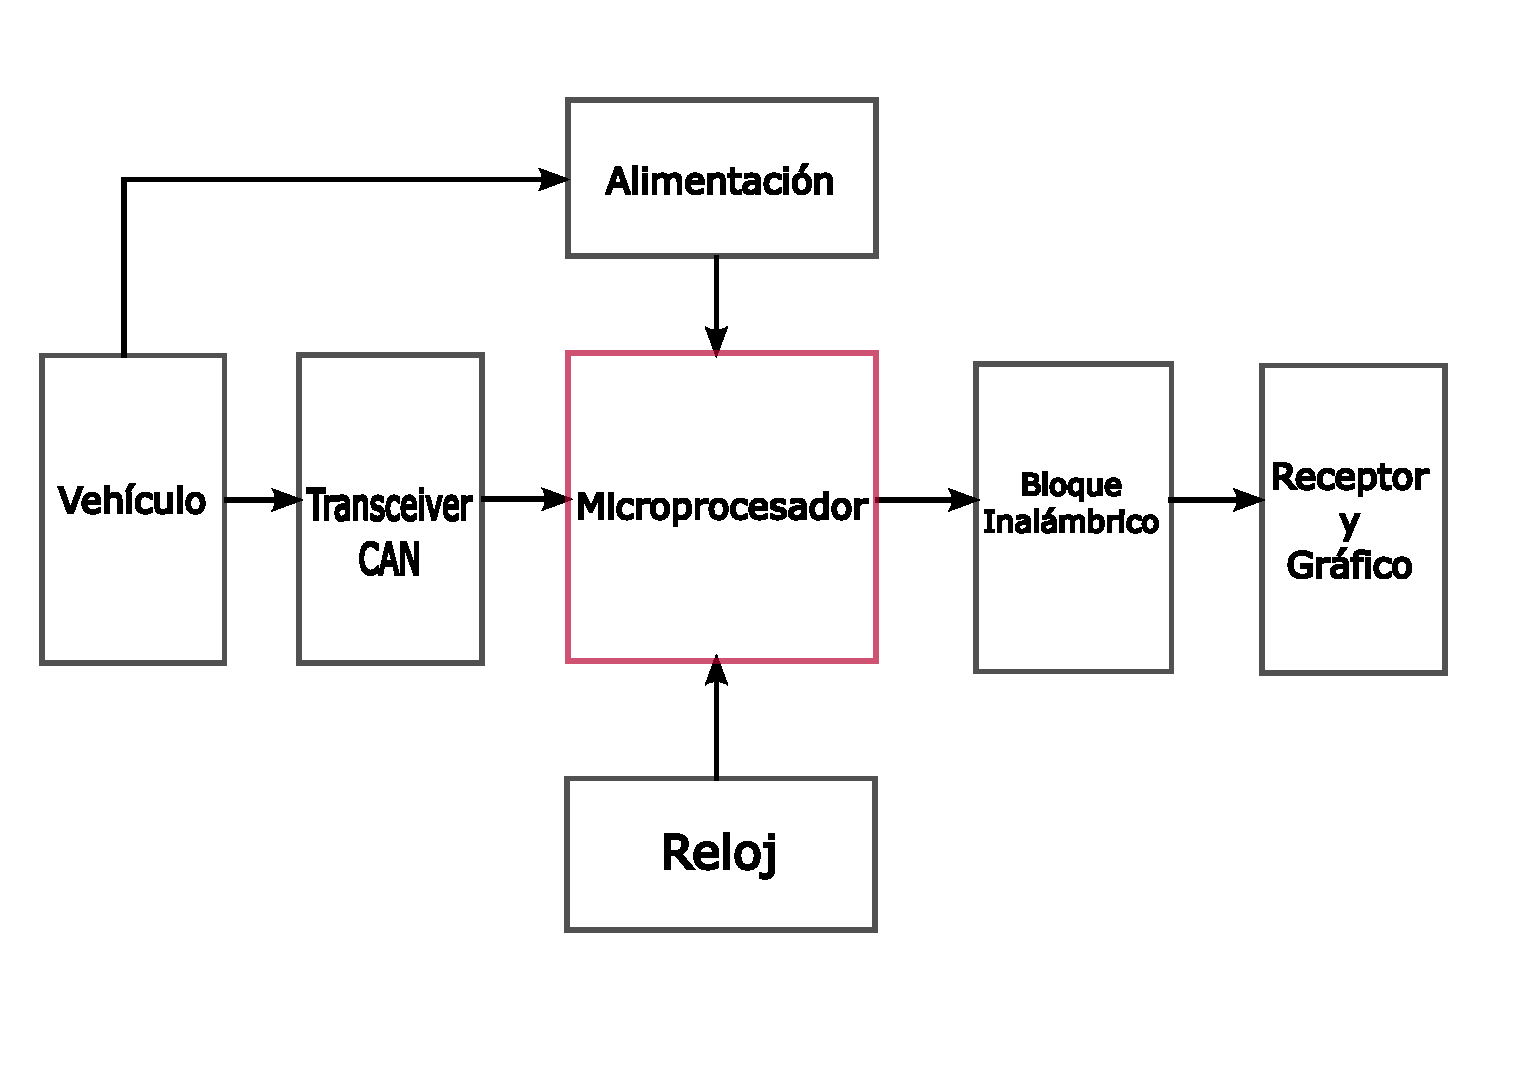
\includegraphics[width=0.9\textwidth]{./Cap4imagen/bloqueHardware.pdf}
	\caption[Diagrama en Bloque del sistema.]{Diagrama en Bloque del sistema.\textbf{ Fuente:}  Elaboración Propia.}
	\label{fig_bloque_c4} % Etiqueta para la referencia.
\end{figure}

% CITAR IMAGEN
%%%%%%%%%%%%%%%%%%%%%%%%%%%%%%%%%%%%%%%%%%%%%%%%%%%%%%%%%%


Para dicho diseño, se utilizará un microcontrolador de la familia PIC (\textit{Peripheral Interface Controller}, por sus siglas en inglés), ya que los PIC son una familia de microcontroladores con amplia documentación técnica y tiene una comunidad de personas activas utilizando estos microcontroladores. 
Son fabricados por \textit{Microchip Tecnhology Inc.} y existe una gran cantidad de modelos con características y prestaciones, esto nos permite escoger el modelo que se ajusta a la necesidad. 
Para el Proyecto se utilizó el PIC18F4580 que incluye internamente un módulo CAN y un módulo serial. 

\section{Implementación del Hardware con el PIC18F4580}
\subsection{Microcontrolador PIC18F4580}

Las características del módulo CAN incorporado en el PIC son las siguientes:
\begin{itemize}
	\item Aplicación del protocolo CAN 1.2,
	CAN 2.0A y CAN 2.0B.
	\item Tramas de datos estándar y extendidas.
	\item 0-8 bytes de longitud de datos.
	\item Tasa de bits programable hasta 1 Mbit / seg.
	\item Totalmente compatible con módulos CAN PIC18XXX8.
	\item Tres modos de funcionamiento:
	\begin{itemize}
		\item Modo 0: El modo tradicional.
		\item Modo 1: Mejora del modo tradicional con
		apoyo DeviceNet.
		\item Modo 2: Modo FIFO con el apoyo de DeviceNet.
		\end {itemize}
		\item Soporte para tramas remotas con el manejo automatizado.
		\item  Seis memorias intermedias programables como RX y TX, 
		almacenamientos intermedios de mensajes.
		\item 16 filtros de aceptancia.
		\item Dos máscaras de filtro de aceptancia completos que pueden ser asignado a cualquier filtro.
		\item Tres buffers de transmisión dedicados.
		\item Temporizador interno~\cite{DaP}.
		\item Modo de bajo consumo.
	\end{itemize}

Para que el PIC pueda realizar sus funciones es necesario programarlo y hemos de escribir un programa que contenga los procesos que el PIC debe ejecutar para manejar el módulo CAN y operar el protocolo. 
Este programa se puede escribir en varios lenguajes de programación, pero los  más utilizados son el ``Assembler'' (ensamblador) y el C. 
En el proyecto se utiliza el lenguaje C por su potencia y robustez para sistemas embebidos, y como compilador del mismo se utiliza CCS (\textit{Custom Computer Services, Inc.}, por sus siglas en inglés), que es un compilador de lenguaje C optimizado para microcontroladore PIC.

Otras características que se aprovecha del PIC18F4580 son: 
\begin{itemize}
\item {\textbf{Reloj:}} Ofrece varias opciones de configuración de la frecuencia de oscilación, permitiendo al usuario escoger según se adapte a sus necesidades.
Para la elección de la frecuencia de oscilación se ha escogido un clock de 16Mhz.
\item {\textbf{Input/Output:}} En este PIC hay 5 puertos diferentes (A, B, C, D y E). El diseño del hardware utiliza estos puertos para posibles expansiones del circuito o del sistema. 
\item {\textbf{Memoria de programa:}} Tiene 32 kbytes de memoria Flash, suficiente para el diseño del programa.
\item {\textbf{Periféricos:}} En el PIC18F4580 aprovechamos el módulo serial EUSART para comunicar los datos procesador a una central~\cite{DaP}.

\end{itemize}


\subsection{Transceiver BUS CAN MCP2551}
El módulo CAN del  PIC18F4580 precisa de un componente externo llamado transceiver CAN. 
Esto es así para proteger el microcontrolador de cortocircuitos o sobretensiones. 
Los transceiver están diseñados para uso en aplicaciones de comunicación BUS CAN en la capa física según la norma ISO 11898. 
El transceiver proporciona una transmisión y recepción de bus diferencial para el controlador CAN y ofrece velocidades de hasta 1Mbps.
El MCP2551 está diseñado para funcionar en ambientes agresivos y cuenta con protección contra sobretensiones, sobrecalentamiento y una amplia gama de modos de servicios. 
El pin 8 ofrece tres modos de funcionamiento: alta velocidad, control de pendiente, y modos de bajo consumo.
El modo de alta velocidad de funcionamiento se selecciona mediante la conexión del PIN 8 a tierra, permitiendo a los transistores de salida del transmisor encender y apagar lo más rápido posible. 
En este proyecto utiliza este modo de funcionamiento.

Las pendientes de subida y bajada de los bits se pueden ajustar mediante la conexión de una resistencia a tierra en el PIN 8, ya que la pendiente del bit es proporcional a la corriente de salida del PIN. 
Este control de la pendiente se implementa aplicando valores a la resistencia externa en el PIN 8. 
Por ejemplo con una resistencia de 10 kohm se logra una pendiente de bit de 15V/us,  y con una resistencia de 100 kohm se logra una pendiente de bit de 2V/us. 
Si se aplica un nivel lógico alto al PIN 8 el transceiver entra en modo standby, para ahorrar energía y vuelve a su estado de trabajo al aplicar un nivel lógico bajo al PIN 8. 

Por último el PIN 5 está disponible como una referencia de tensión, la cual en el proyecto se utiliza la referencia de masa~\cite{sn}.  %$V_{ref}$ 5 está disponible como una referencia de tensión.

\subsection{Módulos inalámbricos Xbee}
 los módulos XBee son soluciones integradas que brindan un medio inalámbrico para la interconexión y comunicación entre dispositivos. Estos módulos utilizan el protocolo de red llamado IEEE 802.15.4 para crear redes POINT-TO-MULTIPOINT (punto a multipunto); o para redes PEER-TO-PEER (punto a punto). Fueron diseñados para aplicaciones que requieren de un alto tráfico de datos, baja latencia y una sincronización de comunicación predecible~\cite{xbee_c4}, en la Figura ~\ref{fig_xbee_4} observamos su apariencia. 
 
 %%%%%%%%%%%%%%%%%%%%%%%%%%%%%%%%%%%%%%%%%%%%%%%%%%%%%%%%%%
\begin{figure}[H]
	\centering
		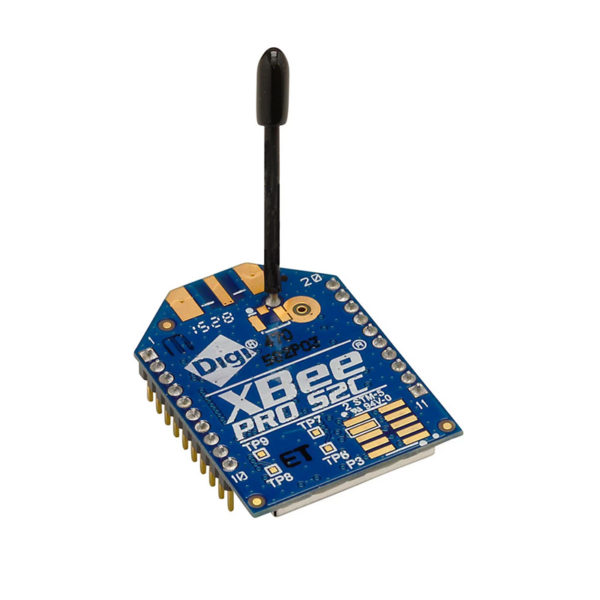
\includegraphics[width=0.6\textwidth]{./Cap4imagen/xbee_modulo.jpg}
	\caption[Fuente de Alimentación.]{Fuente de Alimentación.\textbf{ Fuente:}  \cite{cite_xbee_4}.}
	\label{fig_xbee_4} % Etiqueta para la referencia.
\end{figure}

% CITAR IMAGEN
%%%%%%%%%%%%%%%%%%%%%%%%%%%%%%%%%%%%%%%%%%%%%%%%%%%%%%%%%%

\subsection{Diseño del Hardware}
El montaje implementado es una placa de hardware BUS CAN, basado en el microcontrolador de bajo coste PIC18F4580. La función principal del mismo, es poder leer datos del BUS
CAN y enviarlos a un servidor para mostrarlos en una interfaz gráfica. 
Para realizar la placa PCB (\textit{Printed Circuit Board}, por sus siglas en inglés) se utilizó el software Proteus~\cite{pro},  el cual es un programa de diseño de diagramas y PCBs con autoenrutador. 
Proteus tiene una facilidad de uso y configuración.

En la Figura~\ref{Esch1} se observa el diagrama del bloque de alimentación del hardware que cuenta con un regulador de tensión LM7805 y dos condensadores electrolíticos cuya función es eliminar el rizado de la señal en la entrada del regulador para que la tensión de salida no tenga variaciones de tensión debido a irregularidades de la fuente principal. 

%%%%%%%%%%%%%%%%%%%%%%%%%%%%%%%%%%%%%%%%%%%%%%%%%%%%%%%%%%
\begin{figure}[H]
	\centering
		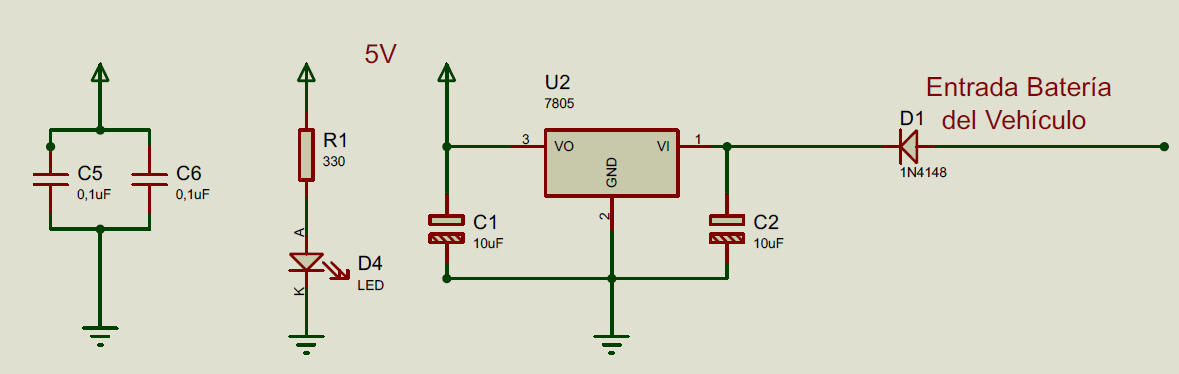
\includegraphics[width=0.6\textwidth]{./Cap4imagen/Fuente5v_4.png}
	\caption[Fuente de Alimentación.]{Fuente de Alimentación.\textbf{ Fuente:} 
	%\cite{sch1}.
	Elaboración Propia.}
	\label{Esch1} % Etiqueta para la referencia.
\end{figure}

% CITAR IMAGEN


%%%%%%%%%%%%%%%%%%%%%%%%%%%%%%%%%%%%%%%%%%%%%%%%%%%%%%%%%%

El Transceiver MCP2551 de Microchips es una interfaz entre el controlador del protocolo BUS CAN que se encuentra en el PIC, y el BUS CAN físico. 
Este chip está formado por un driver que nos convierte las señales que entran por el CANH  y CANL a señales CMOS para tener una lectura correcta de los datos en el PIC. 
La configuración de pines no requiere otros elementos aparte de los propios conectores para  entrada, salida y fuente de alimentación. 
En la Figura~\ref{Esch2} se observa la conexión donde el PIC será el nodo maestro encargado de escanear y procesar los datos provenientes del bus mediante la ayuda del transceiver CAN. 
La misma se conectará a un conector OBD II mediante un conector DB9. 
La alimentación proviene del conector DB9 que irá a extraer la energía de la batería del vehículo.


%%%%%%%%%%%%%%%%%%%%%%%%%%%%%%%%%%%%%%%%%%%%%%%%%%%%%%%%%%%
\begin{figure}[H]
	\centering
		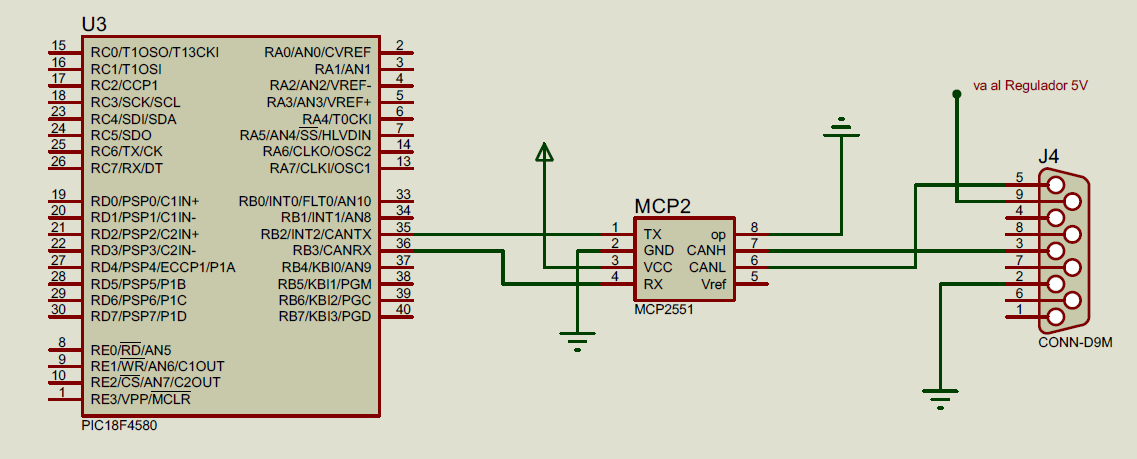
\includegraphics[width=0.9\textwidth]{./Cap4imagen/pic_y_mcp_4.png}
	\caption[Esquemático del Transceiver CAN.]{Esquemático del Transceiver CAN.\textbf{ Fuente:} 
		%\cite{Tu}.
		Elaboración propia}
	\label{Esch2} % Etiqueta para la referencia.
\end{figure}

% CITAR IMAGEN


%%%%%%%%%%%%%%%%%%%%%%%%%%%%%%%%%%%%%%%%%%%%%%%%%%%%%%%%%%%

En la Figura~\ref{Esch3} se observa la incorporación de un módulo inalámbrico Xbee para la comunicación con el servidor de datos. 


%%%%%%%%%%%%%%%%%%%%%%%%%%%%%%%%%%%%%%%%%%%%%%%%%%%%%%%%%%%%%
\begin{figure}[H]
	\centering
		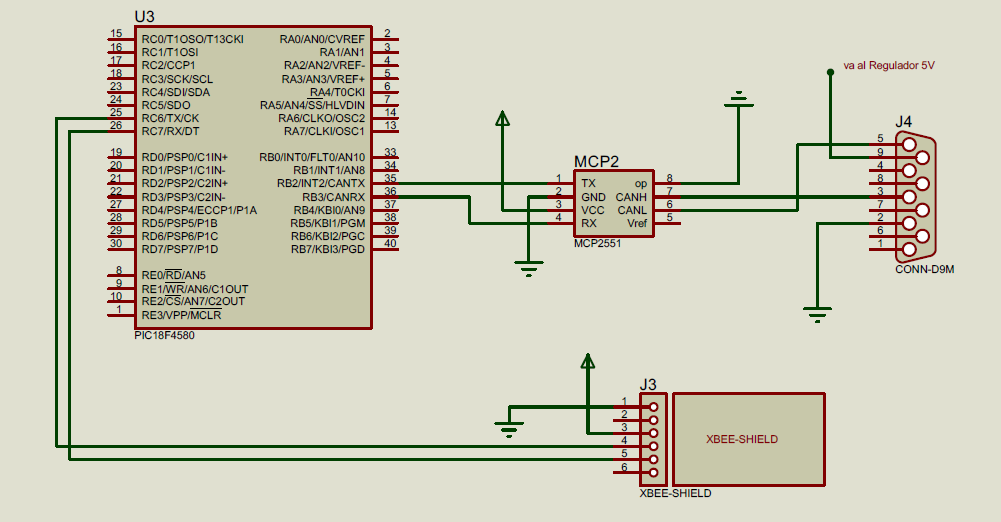
\includegraphics[width=0.9\textwidth]{./Cap4imagen/xbee_4.png}
	\caption[Esquemático PIC y Módulo inalámbrico Xbee.]{Esquemático PIC y Módulo inalámbrico Xbee.\textbf{Fuente:} Elaboración propia.}
	\label{Esch3} % Etiqueta para la referencia.
\end{figure}

% CITAR IMAGEN


%%%%%%%%%%%%%%%%%%%%%%%%%%%%%%%%%%%%%%%%%%%%%%%%%%%%%%%%%%%%%
 En la Figura~\ref{Esch5} que presenta el circuito completo se puede observar los bloques principales del diseño, el bloque de programación y $reset$, el bloque de alimentación y regulación que es alimentado por la batería de 12v del vehículo y luego es reducida a 5v, el bloque de reloj el cual nos da el clock necesario para configurar la velocidad del bus CAN, el bloque inalámbrico para la comunicación a distancia, el bloque transceiver CAN y el bloque de entrada del vehículo. 
 

%%%%%%%%%%%%%%%%%%%%%%%%%%%%%%%%%%%%%%%%%%%%%%%%%%%%%%%%%%%%%

%%%Las distancias indicadas son trim = izquierda abajo
%%%derecha arriba, y debe ir siempre seguido del comando clip.
\begin{figure}[H]
	\centering
		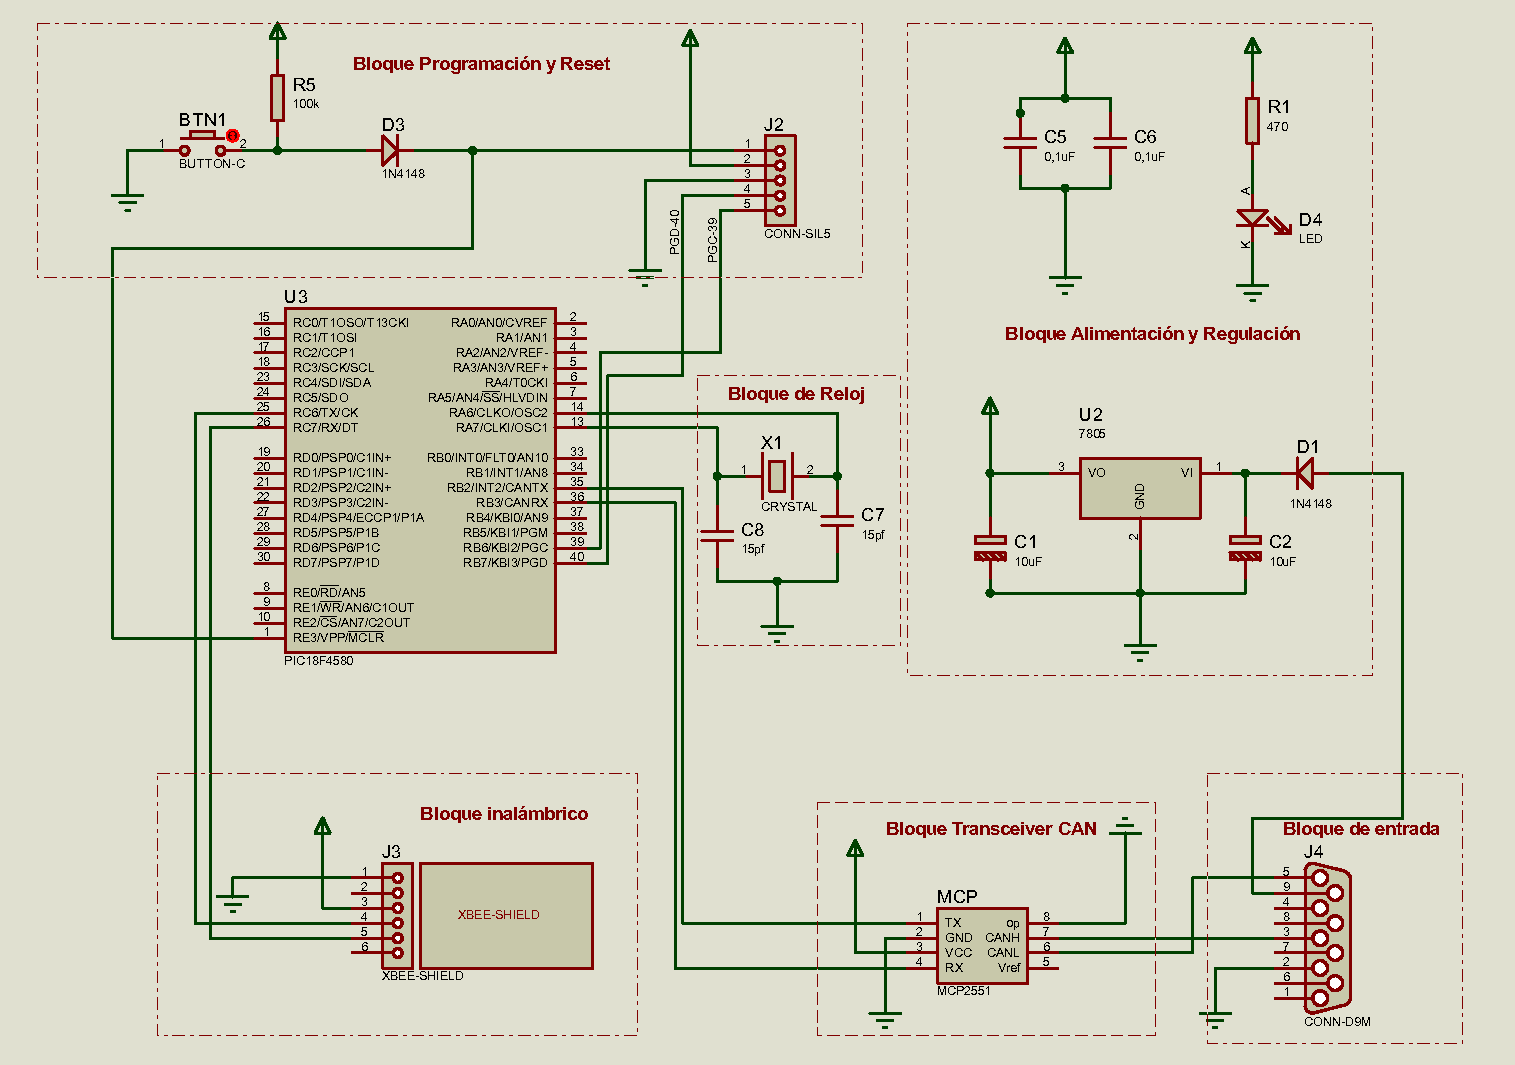
\includegraphics[ width=1\textwidth]{./Cap4imagen/ctocompleto_4.pdf}
	\caption[Diseño del Circuito completo BUS CAN.]{Diseño del Circuito completo BUS CAN.\textbf{ Fuente:} Elaboración propia.}
	\label{Esch5} % Etiqueta para la referencia.
\end{figure}

% CITAR IMAGEN
 En la figura Figura~\ref{Esch6} se puede ver la imagen en PCB y en la que se observa la distribución de los componentes electrónicos en la placa.
%%%%%%%%%%%%%%%%%%%%%%%%%%%%%%%%%%%%%%%%%%%%%%%%%%%%%%%%%%%%%
\begin{figure}[H]
	\centering
		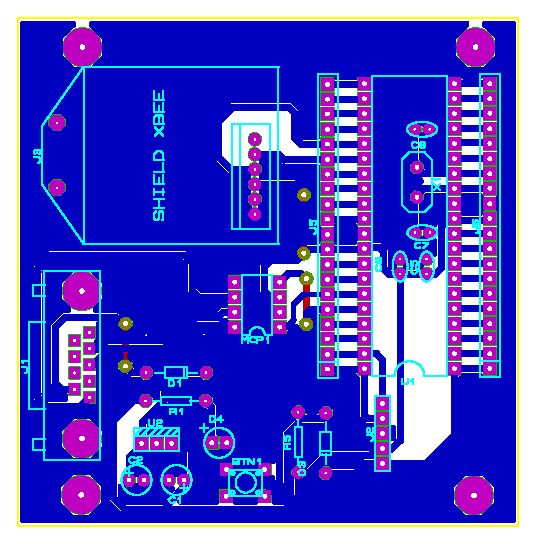
\includegraphics[ width=0.7\textwidth]{./Cap4imagen/pcb_can_4.pdf}
	\caption[ Apariencia del diseño PCB.]{Apariencia del diseño PCB.\textbf{ Fuente:} Elaboración Propia.}
	\label{Esch6} % Etiqueta para la referencia.
\end{figure}

% CITAR IMAGEN


%%%%%%%%%%%%%%%%%%%%%%%%%%%%%%%%%%%%%%%%%%%%%%%%%%%%%%%%%

En la Figura~\ref{Esch7} se muestra las vistas 3D del circuito impreso y ensamblado. 

%%%%%%%%%%%%%    TRANSEIVER         %%%%%%%%%%%%%%%%%%%
\begin{figure}[H]
	\centering
		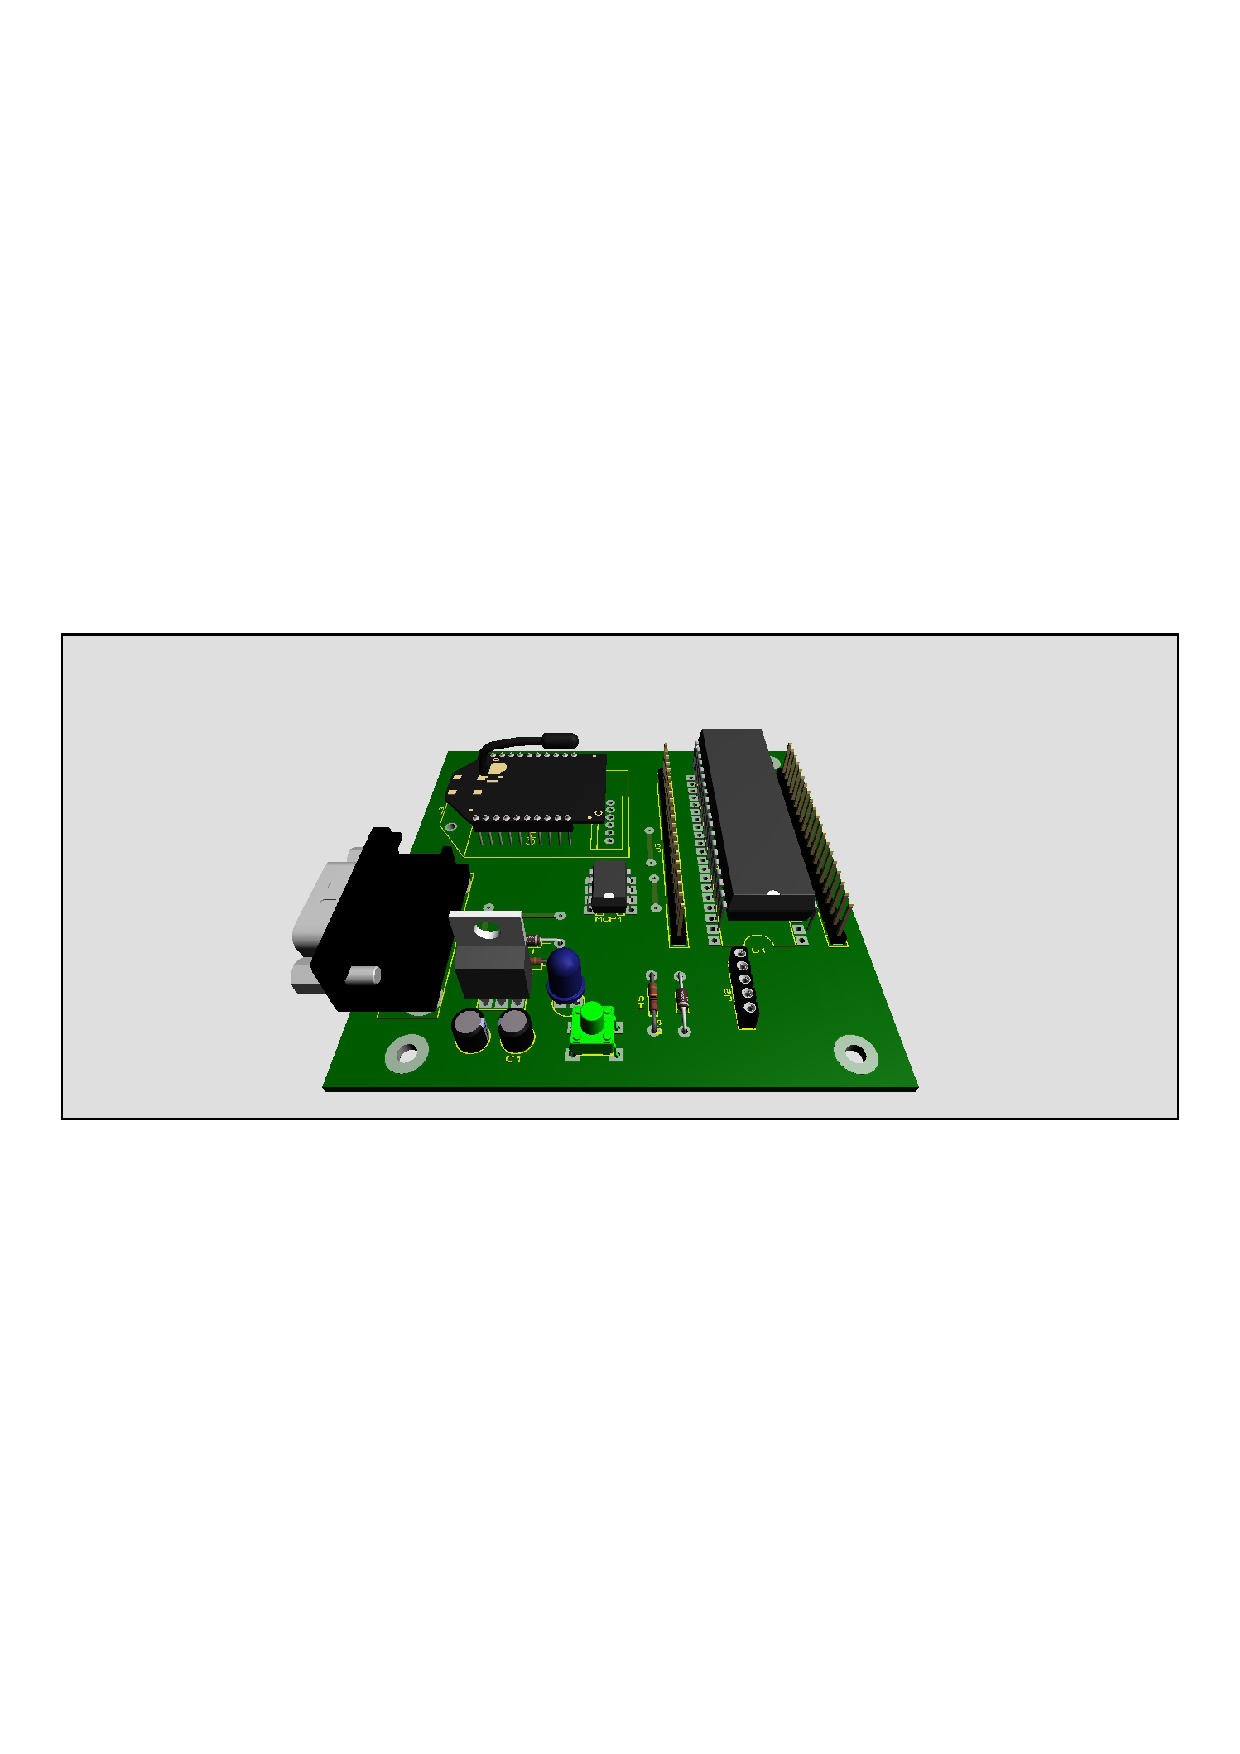
\includegraphics[trim = 10mm 60mm 5mm 50mm, clip, width=0.5\textwidth]{./Cap4imagen/3d_can_4.pdf}
	\caption[Vista 3D del Hardware.]{Vista 3D del Hardware.\textbf{ Fuente:} Elaboración propia.}
	\label{Esch7} % Etiqueta para la referencia.
\end{figure}

% CITAR IMAGEN
%%%%%%%%%%%%%%%%%%%%%%%%%%%%%%%%%%%%%%%%%%%%%%%%%%%%%%%%%%%%%

%%%%%%%%%%%%%%%%%%%%%%%%%%%%%%%%%%%%%%%%%%%%%%%%%%%%%%%%%
\subsection{Proceso de Construcción}
%%%%%%%%%%%%%%%%%%%%%%%%%%%%%%%%%%%%%%%%%%%%%%%%%%%%%%%%

Una vez obtenido el diseño del circuito se procedió a utilizar la máquina CNC (Control Numérico Computarizado)  de la marca Cirqoid para la fabricación del prototipo. 
Este equipo se encuentra en el laboratorio de Sistemas Distribuidos de la FIUNA. 
La CNC Cirqoid se encarga de realizar circuitos eléctricos automáticamente  pudiendo realizar los procesos de desgaste de cobre en una PCB, perforado, dispensación de la pasta de soldar y la colocación componentes electrónicos de tipo SMD (Dispositivos de Montaje Superficial, por sus siglas en inglés) , tomando en cuenta que para cada uno de estos procesos tiene su propio cabezal de trabajo~\cite{cirq}. 
En la Figura~\ref{Esch8} se observa la apariencia del sistema y la elaboración de la placa. 

\begin{figure}[H]
	\centering
		\includegraphics[width=0.7\textwidth]{./Cap4imagen/fresado_4.jpg}
	\caption[Proceso de fabricación del circuito PCB con la máquina CNC.]{Proceso de fabricación del circuito PCB con la máquina CNC.\textbf{ Fuente:} Elaboración propia.}
	\label{Esch8} % Etiqueta para la referencia.
\end{figure}

% CITAR IMAGEN


%%%%%%%%%%%%%%%%%%%%%%%%%%%%%%%%%%%%%%%%%%%%%%%%%%%%%%


%###############################################################################
Una vez culminado el proceso en la Figura~\ref{Esch9} se presenta la placa pcb terminada. 


\begin{figure}[H]
	\centering
	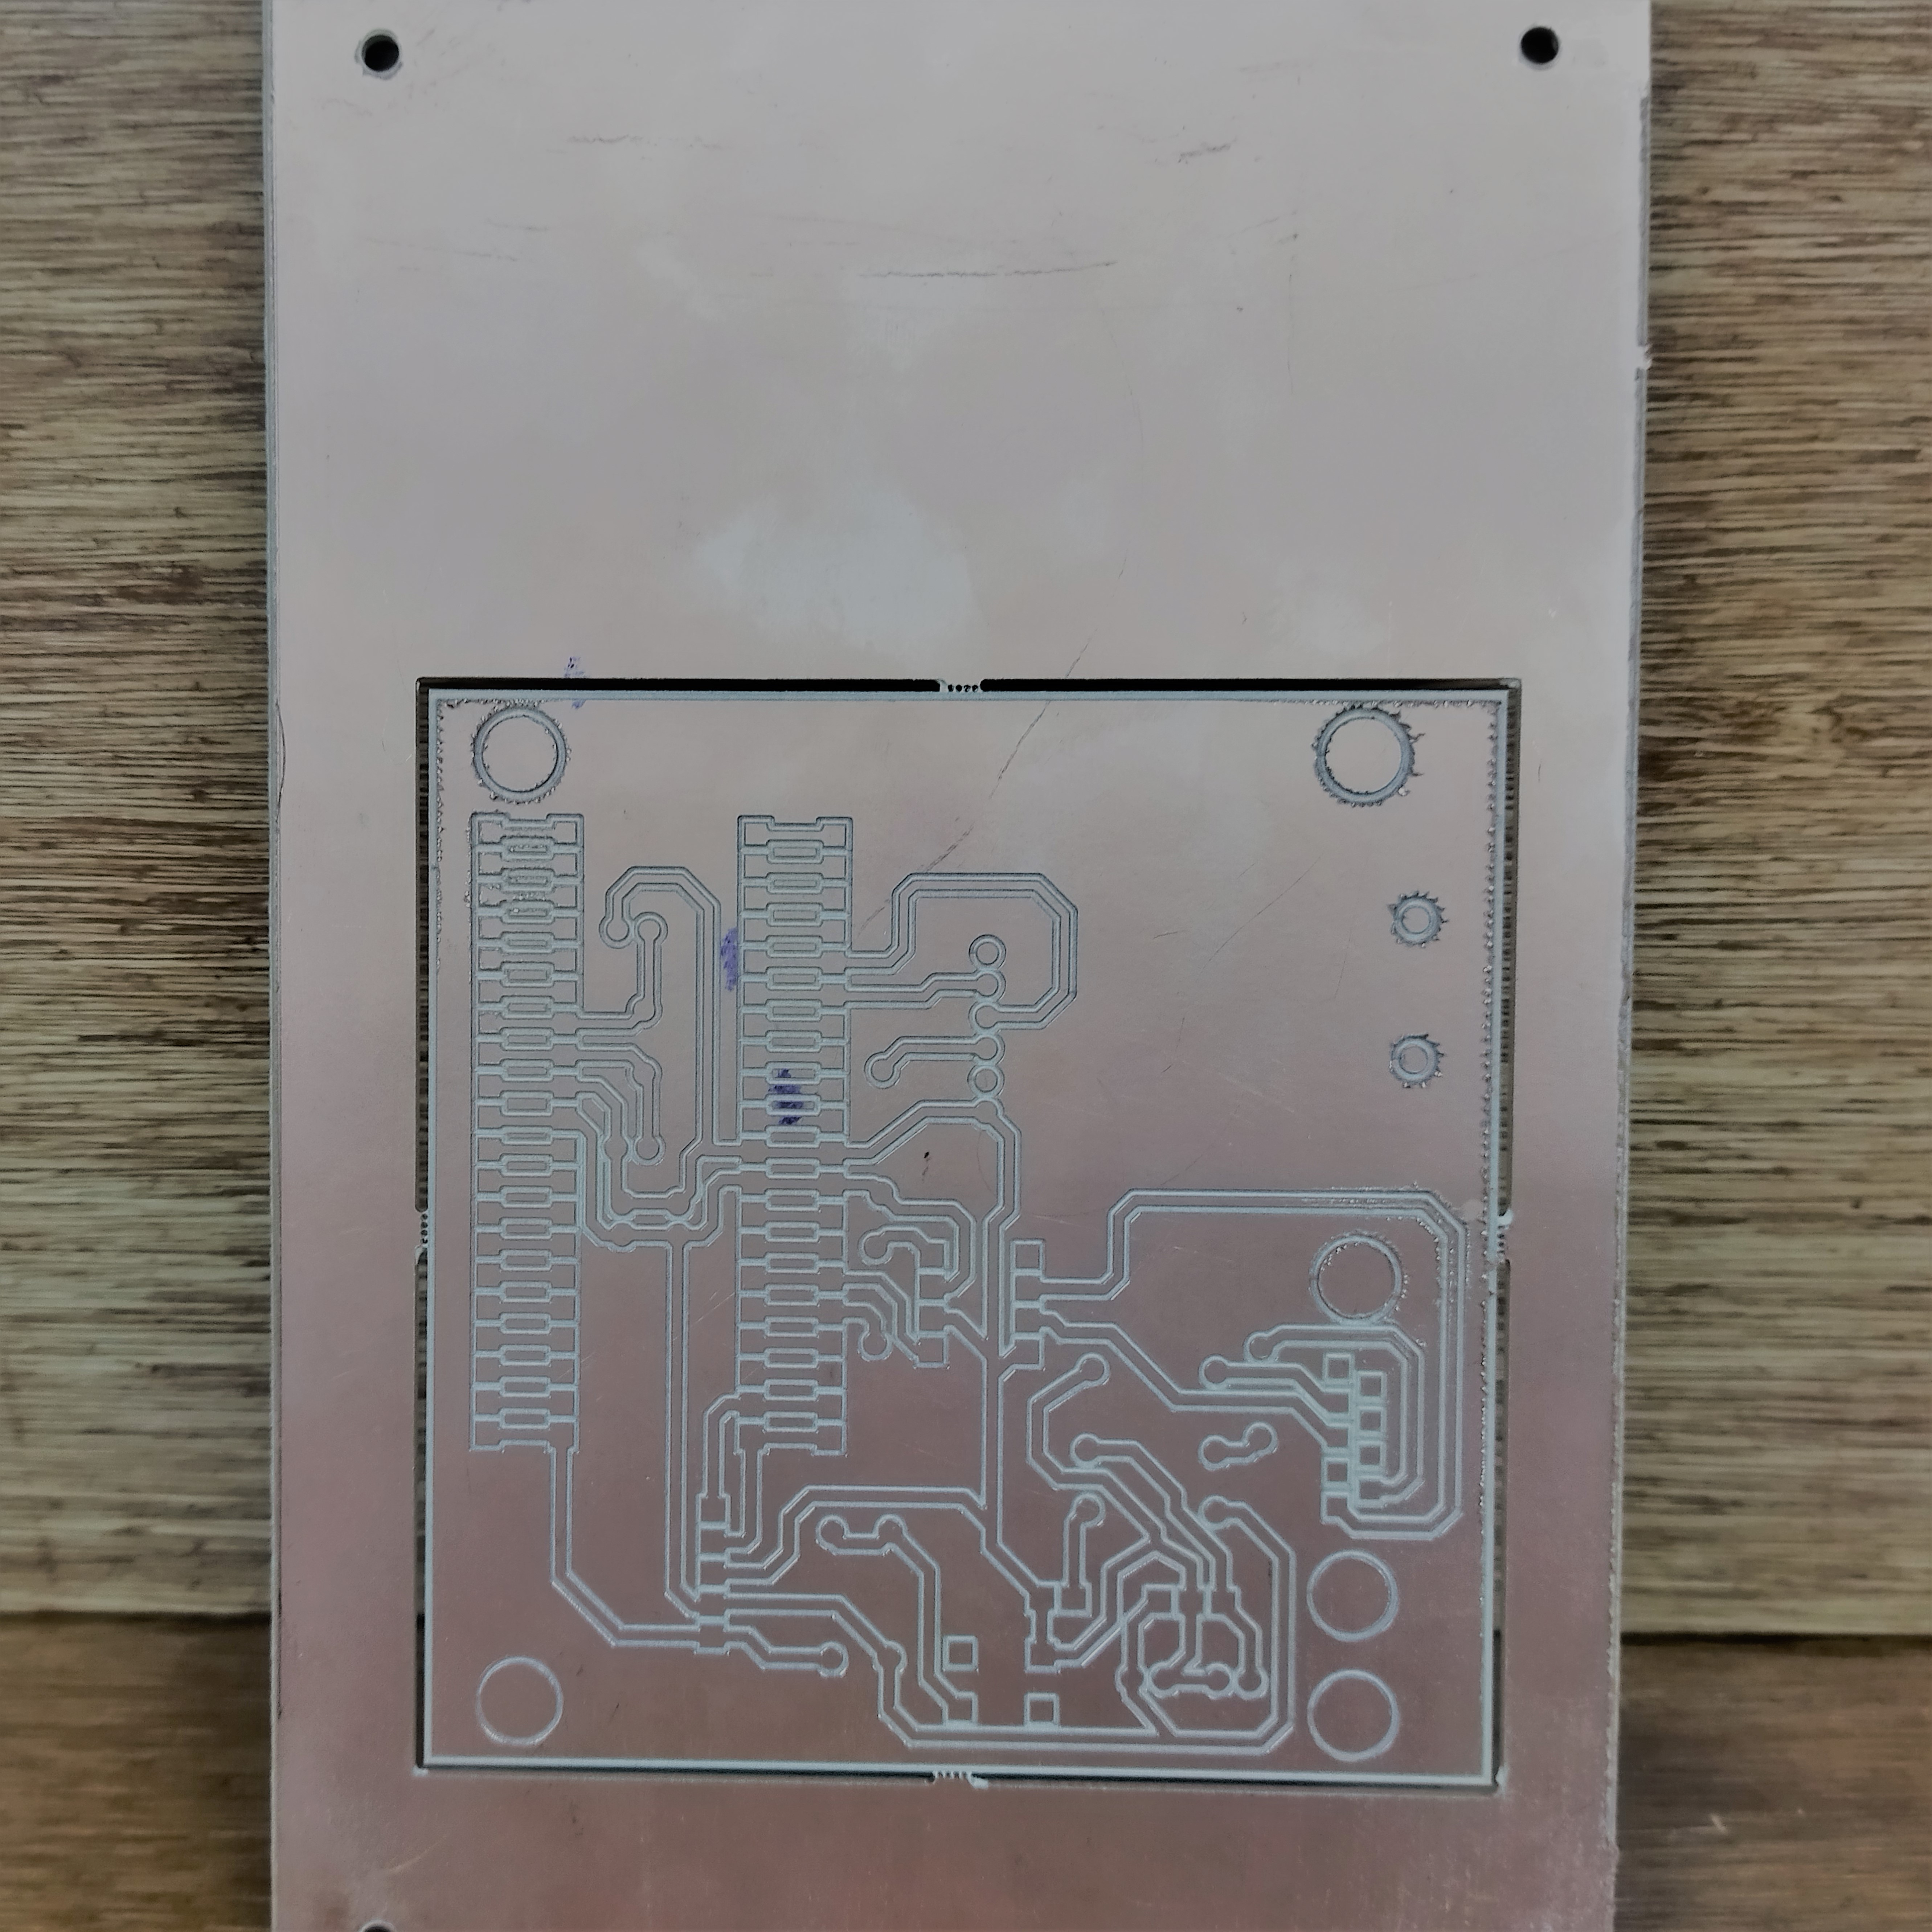
\includegraphics[width=0.5\textwidth]{./Cap4imagen/placa_pcb_4.jpg}
	\caption[Placa impresa.]{Placa impresa. \textbf{ Fuente:} Elaboración propia.}
	\label{Esch9} % Etiqueta para la referencia.
\end{figure}
%###############################################################################

Una vez obtenida el diseño de las pistas del circuito en la placa PCB, se procedió al ensamblado de la misma, resultando el hardware ilustrado en la siguiente Figura~\ref{Esch10}.


%###############################################################################
 
\begin{figure}[H]
	\centering
	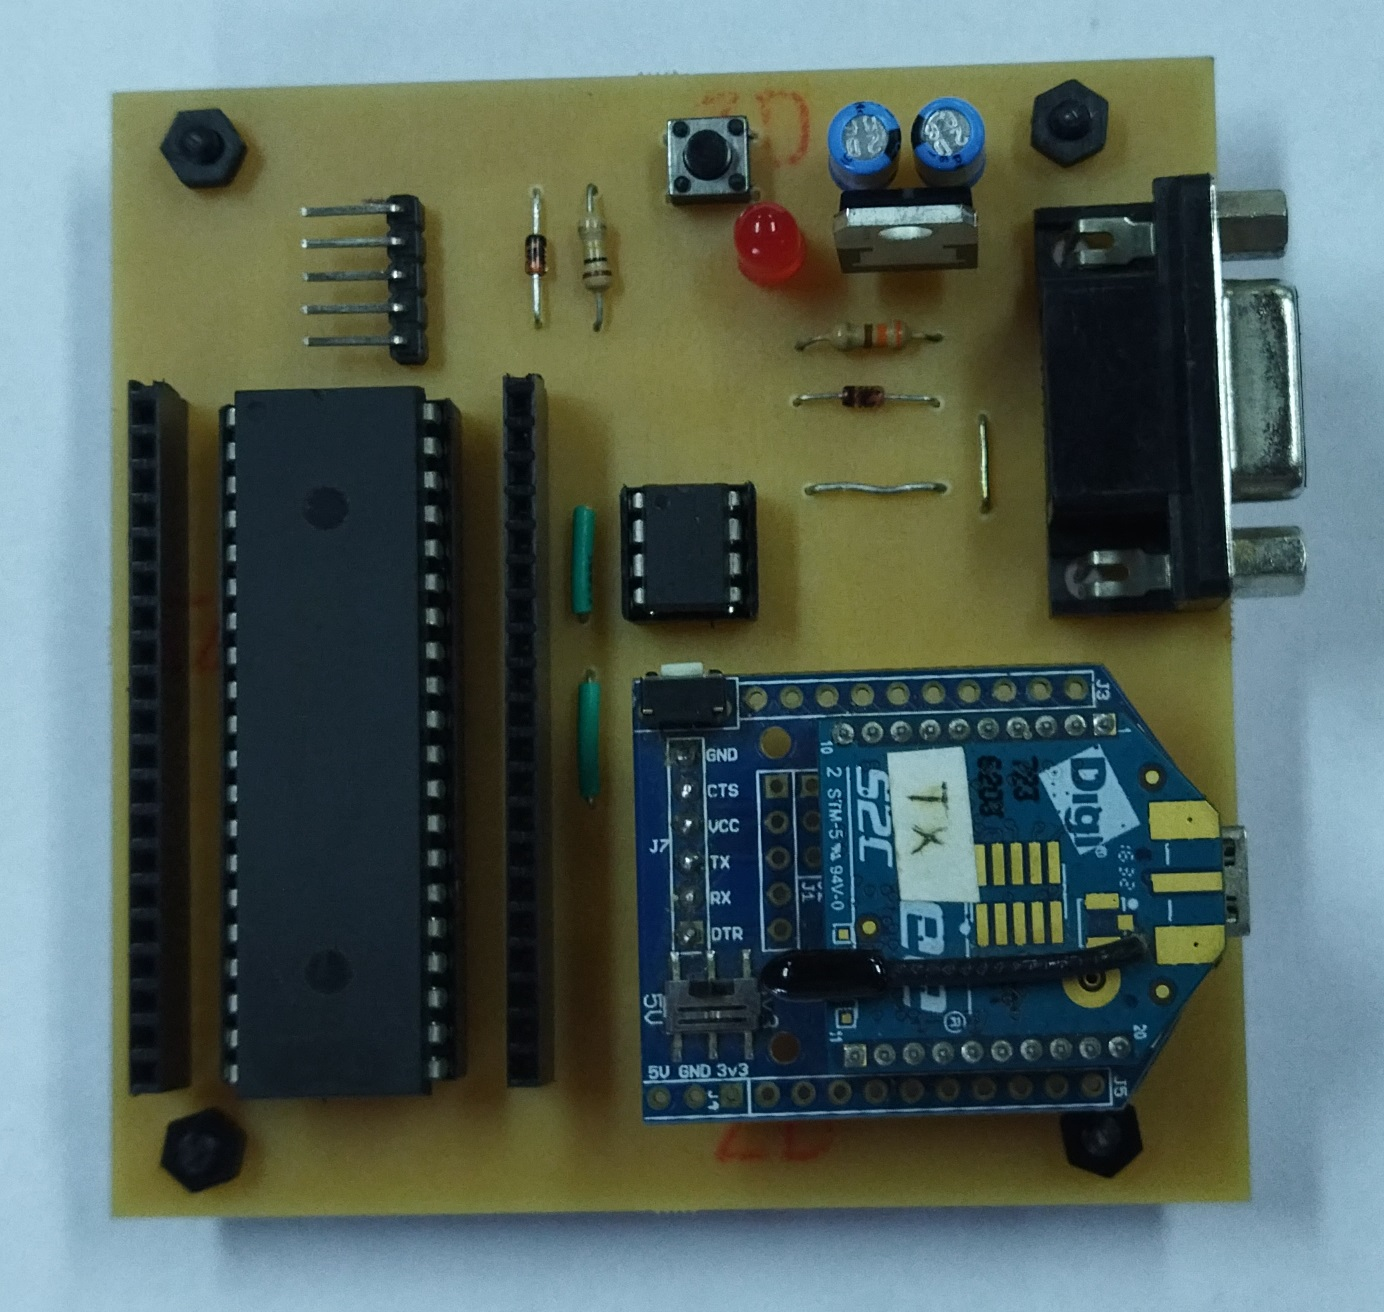
\includegraphics[width=0.5\textwidth]{./Cap4imagen/cto_ensamblado_4.jpg}
	\caption[Vista del Hardware ensamblado.]{Vista del Hardware ensamblado.\textbf{ Fuente:} Elaboración propia.}
	\label{Esch10} % Etiqueta para la referencia.
\end{figure}
%###############################################################################



Para la presentación final se diseña una caja protectora para posar el hardware en su interior, la misma se construyó con una impresora 3D, presentada en la Figura~\ref{3d}  y se observa su presentación y apariencia final en la Figura~\ref{final}, en dónde el elemento cableado es el conector OBD-II que debe conectarse al vehículo motor. 

%###########################
\begin{figure}[H]
	\centering
	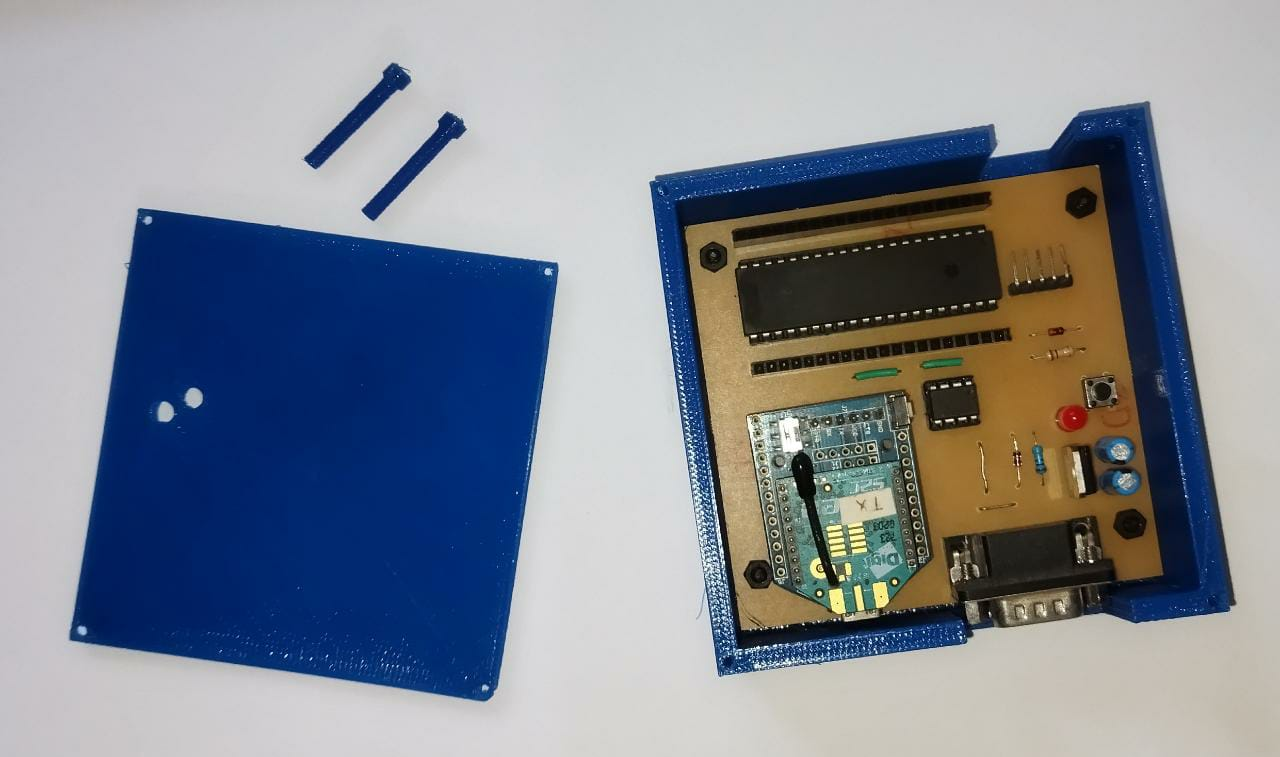
\includegraphics[width=0.5\textwidth]{./Cap4imagen/circuitoycaja_fig.jpeg}
	\caption[Diseño de una caja protectora 3D.]{Diseño de una caja protectora 3D. \textbf{ Fuente:} Elaboración propia.}
	\label{3d} % Etiqueta para la referencia.
\end{figure}
%###############################################################################


%###########################
\begin{figure}[H]
	\centering
	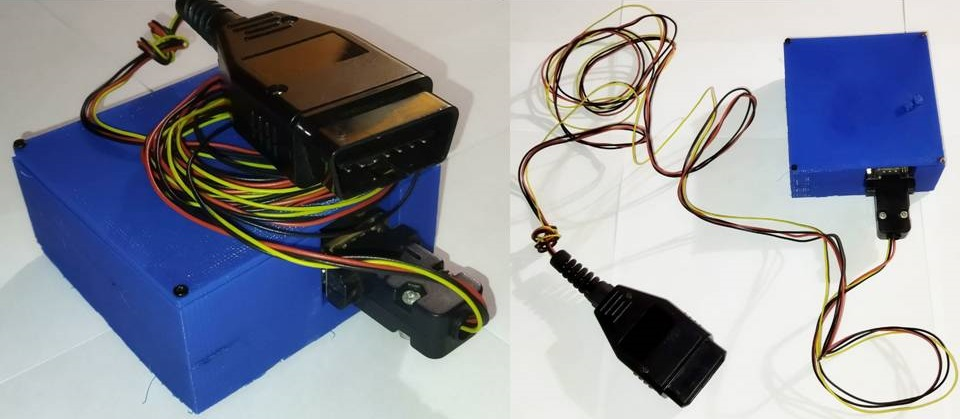
\includegraphics[width=0.5\textwidth]{./Cap4imagen/disenofinal_fig.jpg}
	\caption[Presentación final del hardware CAN.]{Presentación final del hardware CAN. \textbf{ Fuente:} Elaboración propia.}
	\label{final} % Etiqueta para la referencia.
\end{figure}
%###############################################################################




%%%%%%%%%%%%%%%%%%%%%%%%%%%%%%%%%%%%%%%%%%%%5
%%%%%%%%% SIGUIENTE EXcAPITULO 5

%\chapter[Capítulo 5. Diseño del Software]{Diseño del Software}

\section {Diseño del Software del Sistema OBD II y J1939}
Para el diseño del sistema se recurrieron a las siguientes herramientas 
\begin{itemize}
    \item \textbf{IDE PIC CCS: } Para la programación del PIC18F4580 se utilizó como entorno de desarrollo el PIC CCS, que es un entorno de programación en lenguaje C que ya incluye además el compilador del lenguaje \cite{ccs}. 
    
    \item \textbf{Visual Studio Code:} Visual Studio Code es un editor de código fuente y entorno de desarrollo ligero que se ejecuta en un escritorio Windows, macOS y Linux. 
    Viene con soporte incorporado para JavaScript y  Node.js \cite{vsc}, el desarrollo del sistema de visualización OBD II y J1939 se trabaja en Visual Studio Code, facilitando el trabajo tanto para el desarrollo del cliente como del servidor. 
	\item {\bfseries Node.js: }	Node.js es un entorno de ejecución para JavaScript construido con el motor de JavaScript V8 de Chrome, fue ideado como un entorno de ejecución de JavaScript orientado a eventos asíncronos y está diseñado para crear aplicaciones network escalables, para una aplicación dada con esta herramienta puede atenderse muchas conexiones simultáneamente.
	HTTP es un elemento destacado en Node.js, diseñado teniendo en cuenta la transmisión de operaciones con \textit{streaming} y baja latencia. 
	Esto hace que Node.js sea muy adecuado para la base de una librería o un framework web~\cite{nodejs}.
	%Fuente: https://nodejs.org/es/about/
	\item {\bfseries Express.js: } es una infraestructura web rápida, minimalista y flexible para las aplicaciones Node.js. ``Express es una infraestructura de aplicaciones web Node.js minimalista y flexible que proporciona un conjunto sólido de características para las aplicaciones web y móviles. 	
	Con miles de métodos de programa de utilidad HTTP y middleware a su disposición, la creación de una API sólida es rápida y sencilla. 
	Express proporciona una delgada capa de características de aplicación web básicas, que no ocultan las características de Node.js"~\cite{express}. %[https://expressjs.com/es/resources/glossary.html]
	\item {\bfseries Socket.IO: } ``es una biblioteca que permite la comunicación en tiempo real, bidireccional y basada en eventos entre el navegador y el servidor. 
	Consiste en  un servidor Node.js y una biblioteca cliente de Javascript para el navegador"~\cite{socket}. %[ https://socket.io/docs/v4]
	\item {\bfseries Bootstrap: } ``Es un marco de desarrollo que facilita la construcción de páginas web desde el punto de vista estético", \cite{boot}. %[https://getbootstrap.com/]
	\item {\bfseries AdminLTE: } ``Es un diseño de presentación  de código abierto que ofrece un  panel de administración y  un panel de control para la visualización de una página web. 
	Construido sobre Bootstrap, AdminLTE proporciona una gama de componentes receptivos, reutilizables y de uso común"~\cite{admin}. %https://adminlte.io/
	
	Para el diseño de presentación de los datos OBDII y J1939 se utiliza dicha librería por su aspecto amigable desde el punto de vista de un usuario particular. 
	Esta librería solo nos proporciona el diseño de la parte visual y no los algoritmos necesarios para observar la dinámica de las mediciones del vehículo motor, para ello tratamos los datos con el lenguaje javascript. 
	
	\item {\bfseries Canvas-gauge.js:} son componentes minimalistas de código abierto basados en HTML5 para aplicaciones web que simulan un entorno de medidores analógicos. 
	Los medidores  se pueden instalar simplemente usando el administrador de paquetes de nodejs. ``Dependiendo de sus necesidades, existe la posibilidad de instalar una biblioteca de medidores completa o solo la parte que realmente necesita para su proyecto"~\cite{gauge}. %[ https://canvas-gauges.com/]
	
\end{itemize}


\subsection{Diseño del Firmware para el sistema OBDII}

Para mostrar la secuencia de funcionamiento se presenta en la siguiente  Figura~\ref{sobd} un diagrama de secuencia. 
El sistema inicializa el módulo CAN BUS con {\bfseries can-init()} y se habilita las interrupciones del módulo serial y las banderas de interrupciones globales con la función {\bfseries serial-isr()}. 
La interrupción del módulo serial permitirá avisar al microcontrolador cuando los datos recibidos desde un cliente desean consultar datos del bus. 
Este valor es almacenado en la trama CAN para enviarla al sistema del automóvil.

Con la inicialización del módulo CAN bus se procede a configurar los filtros del protocolo, pues nos permitirá recibir solo los datos que nos interesan e ignorará los que no nos sirven, para el Protocolo OBDII permitiremos que solamente leamos las respuesta que nos da la computadora. 
De manera estándar la computadora del vehículo envía mensajes con el siguiente rango de identificadores: 0x7E0 a 0x7E8. 

Una vez tenemos esto podemos proceder a la consulta enviando una trama CAN al bus con la función {\bfseries can-putd(id, data)} y se espera a que el sistema vehicular nos responda. 
Al recibir la respuesta del sistema auto motor con la función {\bfseries cant-getd(id,data)} dichos datos pasan por un procesamiento para interpretar los bits recibidos en los campos de datos. 
Para ello se utiliza los documentos OBD-II SAE J1979 donde indica los procedimientos matemáticos para el calculo de las mediciones. 

Luego se envía dichos datos a nuestro servidor con la función {\bfseries print()}. 
El formato de envío de mensaje se llama JSON, es un tipo de formato para el intercambio de datos entre software basado en texto y se utiliza mucho para el desarrollo web. 
Esto permitirá que en el lado del servidor podamos manipular mejor los datos enviados por el PIC, el formato JSON que utiliza el sistema OBD-II se ve observa en la Tabla~\ref{tabla:jsoncan}. 


%%%%%%%%%%%%%%%%%%%%% tabla %%%%%%%%%%%%%%%%%%%%%%%%%%%%%%%%
\begin{table}[H]
\begin{center}
\begin{tabular}{l c c  }
\toprule
\textbf{Esquema de datos JSON}  & &   \\ 

\{            &  &    \\   
  ``A" : ``F004",  &  &  \\
  ``B" :  ``04",   &  &   \\  
  ``C : ``FF",    &  &   \\  
  ``D : ``[0,1,2,3,4,5,6,7]", & &  \\ ``Value: ``100""  &  &  \\    
  \}          &  & \\ \bottomrule
\end{tabular}
\caption{Formato de envío JSON de los campos del protocolo CAN.}
\label{tabla:jsoncan}
\end{center}
\end{table}


donde A, B, C y D son campos de datos del protocolo y ''value'' es el valor calculado de la respuesta del vehículo, los valores 00, 11, 22, 33 y 44 son valores asignados para ejemplo. 

 


%%%%%%%%%%%%%%%%%%%%%%%%%%%%% DIAGRAMA DE SECUENCIA FIRMWARE OBD


\begin{figure}[H]
	\centering
	\begin{center}
		\begin {sequencediagram}
\newthread {main}{Main}
\newinst [1]{conf}{initCAN}
\newinst [1]{serial}{PuertoSerial}
\newinst [2]{can}{BufferCAN}

\newinst [1]{int}{interrupción}
 

%%%%%enlaces%%%%%

\begin{call}{main}{cant-init()}{conf}{true}
\end{call}
\begin{call}{main}{serial-init()}{serial}{true}
\end{call}
\begin{call}{main}{serial-isr()}{int}{return PID}
\end{call}


\begin{sdblock}[blue!10]{Loop}{}
	

	\begin{call}[2]{main}{can-putd(id,data)}{can}{return true/false}
	\end{call}


	\begin{call}[2]{main}{can-getd(id,data)}{can}{return data}
	\end{call}
	
    
    \begin{call}[2]{main}{print(JSON)}{serial}{void}
	\end{call}
    
    
	\end{sdblock}
\end {sequencediagram}
	\end{center}
	%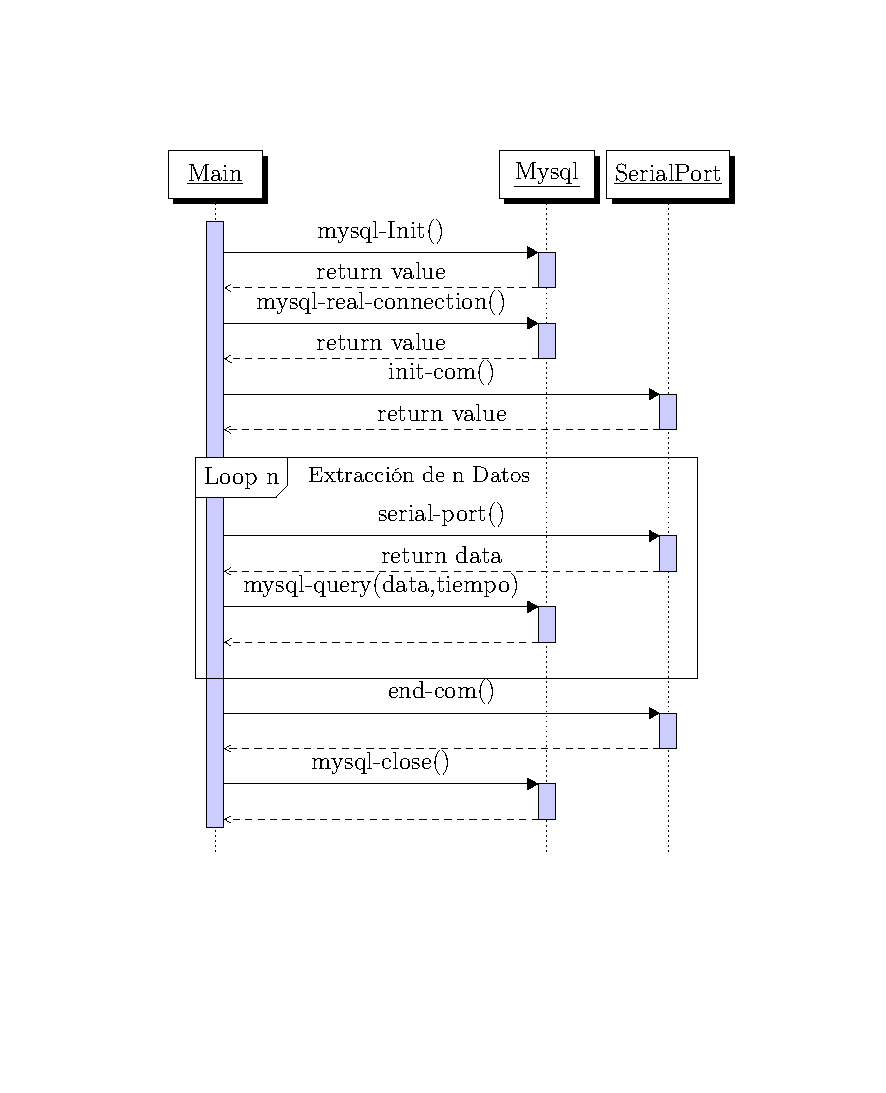
\includegraphics[width=1\textwidth]{./Cap5imagen/c.pdf}
	\caption[Diagrama de Secuencia Firmware OBDII.]{Diagrama de Secuencia Firmware OBDII \textbf{ Fuente:} Elaboración Propia.}
	\label{sobd} % Etiqueta para la referencia.
\end{figure}

%%%%%%%%%%%%%%%%%%%%%%%%


\subsection{Diseño del Firmware para el sistema J1939}

Para presentar la secuencia del procedimiento del protocolo J1939 nos apoyamos del diagrama de secuencia vista en la Figura~\ref{sj}.
Las partes más importantes son inicializar el módulo CAN, el módulo serial, el Timer2 y se habilitan las interrupciones necesarias. 
El {\bfseries timer2()} se utiliza como temporizador para medir los tiempos de comunicación con el bus. 
Se comienza con la función {\bfseries j1939init()}, dicha función provee de un nombre y una dirección al dispositivo para que pueda conectarse a la red, además envía un ''Address claim'' para reclamar una dirección. 
Si dicho reclamo es exitoso podemos empezar la comunicación con cualquier dispositivo, en caso contrario podemos cambiar automáticamente nuestra dirección e iniciar de nuevo el proceso hasta tener éxito. 
{\bfseries serial-init()} inicializa el puerto serial necesario para recibir y enviar información al servidor y con {\bfseries serial-isr() } recibimos los datos del servidor para indicar al microprocesador la lectura de los mensajes que deseamos del bus J1939. 

Una vez conectados se leen los mensajes presentes en el bus con la función {\bfseries J1939GetMessage()} y recuperamos el PGN (\textit{Parameter Group Number}, por sus siglas en inglés) , 
Dichos parámetros PGN pueden ser decodificados utilizando como referencia el documento SAE j1939-71 que nos proporciona las operaciones matemáticas para obtener la medición del sensor deseado.  
Todo ello se realiza con la función {\bfseries lecturaParametro()}.
Una vez leído y codificado pasamos los datos al servidor, con la cadena JSON  mediante la función {\bfseries print(JSON)}, dicho formato se representa en la Tabla~\ref{tabla:json}. 


%%%%%%%%%%%%%%%%%%%%% tabla %%%%%%%%%%%%%%%%%%%%%%%%%%%%%%%%
\begin{table}[H]
\begin{center}
\begin{tabular}{l c c  }
\toprule
\textbf{Esquema de datos}  & &   \\ 

\{            &  &    \\   
  ``PG" : ``F004",  &  &  \\
  ``DA" :  ``04",   &  &   \\  
  ``SA : ``FF",    &  &   \\  
  ``Data : ``[0,1,2,3,4,5,6,7]", & &  \\  
  ``Value: ``100""  &  &  \\    
  \}          &  & \\ \bottomrule
\end{tabular}
\caption{Formato de envio JSON, desde el microcontrolador al Servidor.}
\label{tabla:json}
\end{center}
\end{table}

Donde PG significa Parámetro de Grupo, DA es Dirección de destino, SA dirección de origen, Data son los 8 bytes del bus can recibidos y ''Value'' es el dato calculado real para visualizar en el lado del cliente.





%%%%%%%%%%%%%%%%%%%%%%%%%%%%% DIAGRAMA DE SECUENCIA FIRMWARE j1939

\begin{figure}[t]
	\centering
	\begin{center}
		\begin {sequencediagram}
\newthread {main}{Main}


\newinst [1]{serial}{PuertoSerial}
\newinst [0]{name}{Init}
\newinst [1]{can}{BufferCAN}

\newinst [0]{pgn}{PGN}
\newinst [0]{int}{interrupción}
 

%%%%%enlaces%%%%%

\begin{call}{main}{J1939init()}{name}{true}
	\begin{call} 
		{name}{address claim}{can}{true-false}
	\end{call}
\end{call}

\begin{call}{main}{timer2()}{name}{true}
\end{call}

\begin{call}{main}{serial-init()}{name}{true}
\end{call}

\begin{call}{main}{serial-isr()}{int}{return PID}
\end{call}


\begin{sdblock}[blue!10]{Loop}{}

	\begin{call}[2]{main}{j1939GetMessage()}{can}{return data}
	\end{call}
	
	\begin{call}[2]{main}{lecturaParametro}{pgn}{true}\end{call}
    
    \begin{call}[2]{main}{print(JSON)}{serial}{void}
	\end{call}
    
    
	\end{sdblock}
\end {sequencediagram}
	\end{center}
	%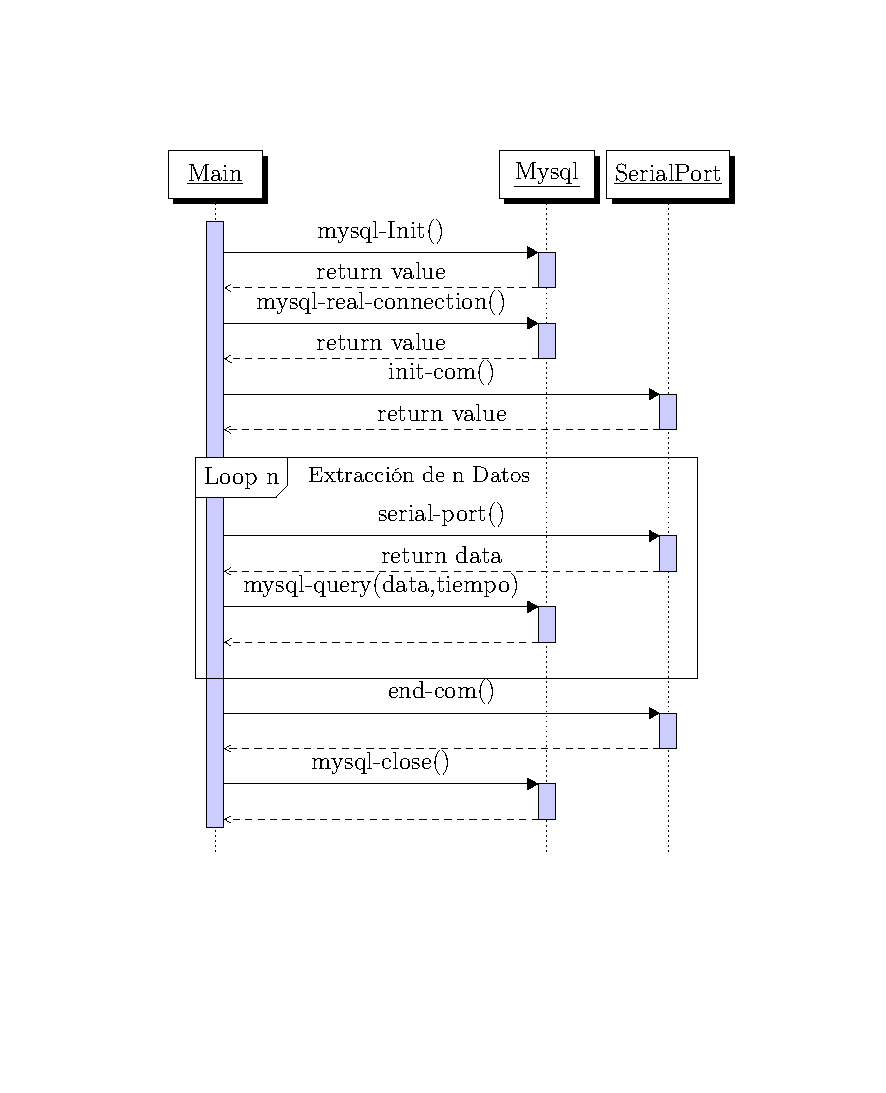
\includegraphics[width=1\textwidth]{./Cap5imagen/c.pdf}
	\caption[Diagrama de Secuencia Firmware OBDII.]{Diagrama de Secuencia Firmware OBDII \textbf{ Fuente:} Elaboración Propia.}
	\label{sj} % Etiqueta para la referencia.
\end{figure}

%%%%%%%%%%%%%%%%%%%%%%%%

\subsection{Diseño del Servidor BUS CAN}
En la \textbf{Figura~\ref{snode}} se detalla el diagrama de secuencia del sistema servidor BUS CAN, para el funcionamiento del programa requeriremos los módulos de http(), express(), y socket(). Una vez inicializados escuchamos el puerto socket para encontrar conexiones al sistema y al mismo tiempo escuchamos el puerto serial con {\bfseries parser.on()} por el cual se recibe datos del vehículo mediante el dispositivo CAN. 
Una vez detectada una conexión web del cliente,  el servidor  procede a enviar los datos del puerto serial al cliente mediante la conexión  {\bfseries socket.emit()}. Estos datos son enviados en formato JSON para un mejor procesamiento de los mismos,  así el cliente recibe constantemente los datos actualizados del vehículo automotor. 

%%%%%%%%%%%%%%%%%%%%%%%%%%%%% DIAGRAMA DE SECUENCIA SERVIDOR

\begin{figure}[t]
	\centering
	\begin{center}
		%%%%%%%%%%%%%%%%%%%%%%%%%%%%%%%%%%%%%%%%%%%%
\begin {sequencediagram}

\newthread [blue!20] {main}{main}
\newinst [1]{require}{Require}
\newinst [1]{serial}{PortSerial}
\newinst [1]{socket}{Socket}
\newinst [2]{cliente}{Cliente}


\begin{call} {main}{call}{require}{http()}
\end{call}

\begin{call}{main}{call}{require}{express()}
 \end{call}

 \begin{call}[1]{main}{call}{require}{socket()}
 \end{call}

\begin{call} {main}{parser.on()}{serial}{True}
	\begin{call}{serial}{socket.emit()}{socket}{true}
			\begin{call}{socket}{data(JSON)}{cliente}{true}
			\end{call}
	\end{call}
	
\end{call}
\end {sequencediagram}
	\end{center}
	%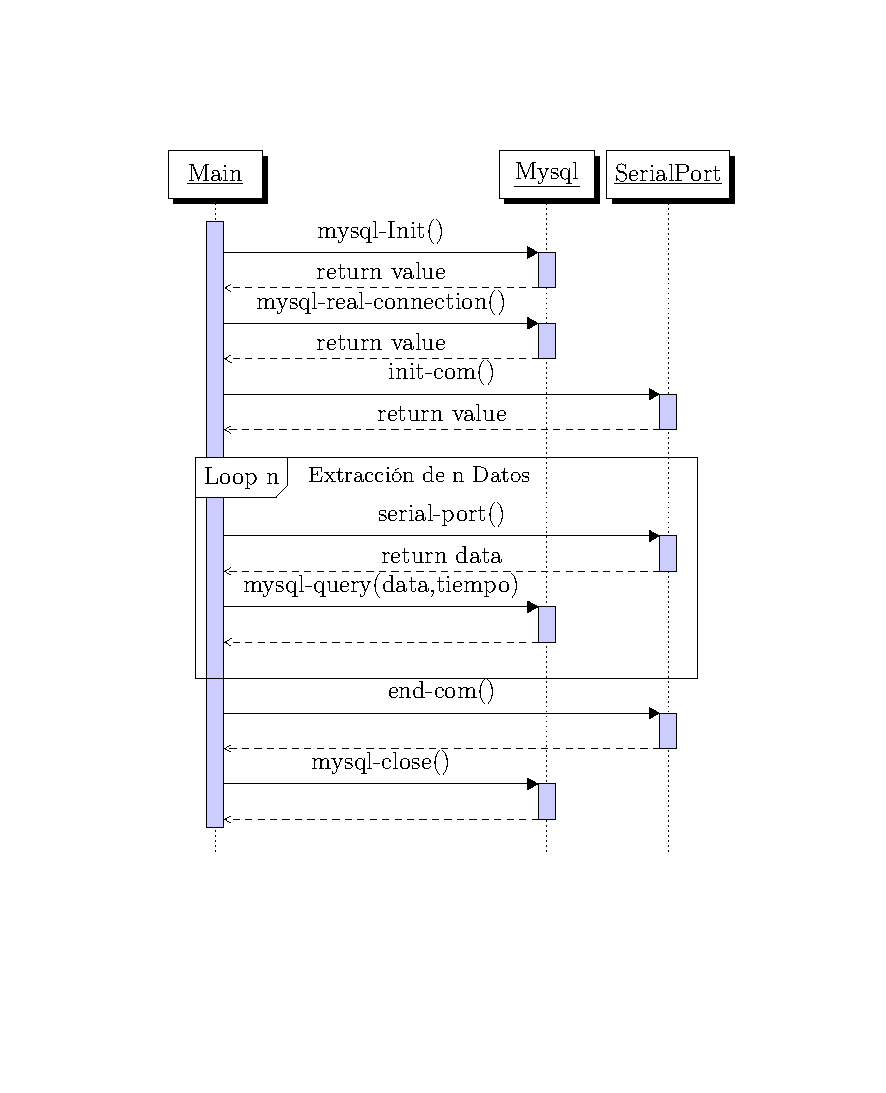
\includegraphics[width=1\textwidth]{./Cap5imagen/c.pdf}
	\caption[Diagrama de Secuencia Servidor CAN.]{Diagrama de Secuencia Servidor CAN \textbf{Fuente:} Elaboración Propia.}
	\label{snode} % Etiqueta para la referencia.
\end{figure}

%%%%%%%%%%%%%%%%%%%%%%%%




\subsection{Diseño de Software para el cliente de Interfaz de Datos BUS CAN}


Para la aplicación en el navegador se utiliza un script de  javascript del lado del cliente, este script visualiza los datos provenientes de la conección socket del servidor en una gráfica entendible para los usuarios. 
La función {\bfseries on()} de la librería socket.io se encarga de escuchar los datos provenientes del servidor y una vez recibidos pasamos dichos datos a las librerías de gráficos utilizadas y se corre un algoritmo de animación. 
Dichas librerías junto con el algoritmo se encargan de gestionar los datos para producir efectos de movimiento y experiencia de animación para el usuario. 
Estas funciones se ejecutan por cada dato recibido desde el servidor y cada 1 segundo, la función {\bfseries update(data)} se encarga de esta rutina de actualización. 
El siguiente diagrama en secuencia en la \textbf{Figura \ref{cweb}} detalla la situación: 
%%%%%%%%%%%%%%%%%%%%%%%%%%%%% DIAGRAMA DE SECUENCIA CLIENTE

\begin{figure}[H]
	\centering
	\begin{center}
		%%%%%%%%%%%%%%%%%%%%%%%%%%%%%%%%%%%%%%%%%
\begin {sequencediagram}

\newthread [blue!20] {web}{Main}
\newinst [1]{socket}{Socket}
\newinst [1]{chart}{Chart}

\newinst [3]{servidor}{Servidor}

%\begin{call}[1]{call} {}{}{}{}\end{call}
\begin{call}[1]{web}{on()}{socket}{data}
	\begin{call}[1]{socket}{socket.on()}{servidor}{data(JSON)}\end{call}
\end{call}

\begin{sdblock}[blue!10]{SetInterval}{Cada 1000ms}
	\begin{call}[1]{web}{update(data)}{chart}{true}\end{call}
\end{sdblock}

\end {sequencediagram}
	\end{center}
	%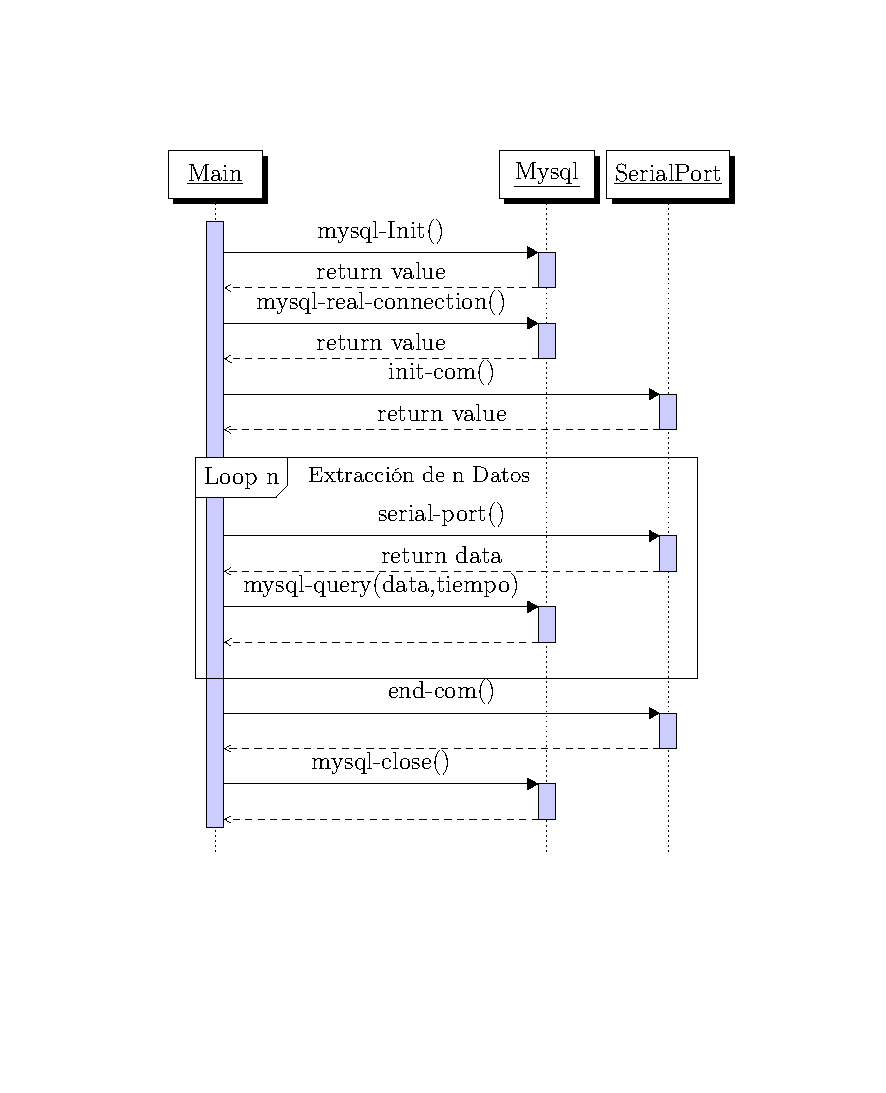
\includegraphics[width=1\textwidth]{./Cap5imagen/c.pdf}
	\caption[Diagrama de Secuencia Cliente Web.]{Diagrama de Secuencia Cliente Web \textbf{ Fuente:} Elaboración Propia.}
	\label{cweb} % Etiqueta para la referencia.
\end{figure}

%%%%%%%%%%%%%%%%%%%%%%%%
%%%%%%%%%%%%%%%%%%%%%%%%%%%%diagrama cliente
	

%%%%%%%%%%%%%%%%%%%%%%%%%%%%%inserta el diagrama

 
%%%%%%%%%%%%%%%%%%%%%%%%%%%

%%%%%%%%%%%%%%%%%%%%%%%%%%%%



%%% GITHUG
Los códigos del proyecto se encuentra en repositorios de github, se pasa a explicar su contenido en la siguiente lista: 
\begin{itemize}
    \item En \cite{githw} se encuentra los archivos de desarrollo del Hardware prototipo para el manejo del protocolo BUS CAN, los mismos fueron hechos en el software Proteus y además se encuentra los archivos gerber del circuito, también se encuentra los modelos de vista 3D de algunos componentes utilizados.  
    
    \item En \cite{gitfirm} se encuentra los códigos, en lenguaje C, del microprocesador PIC18F4580 para configurar y controlar el módulo CAN, además de la programación del estándar OBD II.
    
    \item En \cite{gitj} se encuentra los códigos, en lenguaje C, de los códigos del microprocesador PIC18F4580 para el manejo del estándar J1939.
   
   
    \item En \cite{gitnode} se encuentra los códigos del programa servidor para el sistema de visualización de datos, contiene un archivo ``readme" que explica paso a paso el proceso de instalación del sistema y las herramientas requeridas.  
  
\end{itemize}




















\chapter[Pruebas y Resultados Experimentales]{Pruebas y Resultados Experimentales}

En este capitulo se presentan el funcionamiento del simulador para el estándar CAN J1939 y  las  pruebas de comunicación realizadas con dicho equipo para observar el funcionamiento del protocolo,  además, se presentan pruebas de comunicación realizadas con vehículos reales para el estándar OBD-II, logrando obtener datos de los sensores presentes, luego un análisis de las fallas presentadas durante las pruebas, y se concluye con el análisis financiero del desarrollo del producto.

\section{Simulador SAE J1939}

El simulador Au-SAE J1939 Versión 2.00A es un dispositivo capaz de proveer la mayoría de las señales de la norma SAE J1939. 
Una topología de red típica SAE J1939 se ilustra en la Figura~\ref{TPSAE} en dónde el simulador se conecta al bus mediante una resistencia interna de 120 ohmios, además trae consigo un conector RS-232 para utilizarlo con una Computadora en caso de ser necesario. 
Este simulador es proporcionado por la empresa Electrónica Au Grup para utilizarlo en las pruebas de sistemas SAE J1939, en la Figura~\ref{Sim} se observa su apariencia. 

\begin{figure}[H]
	\centering
		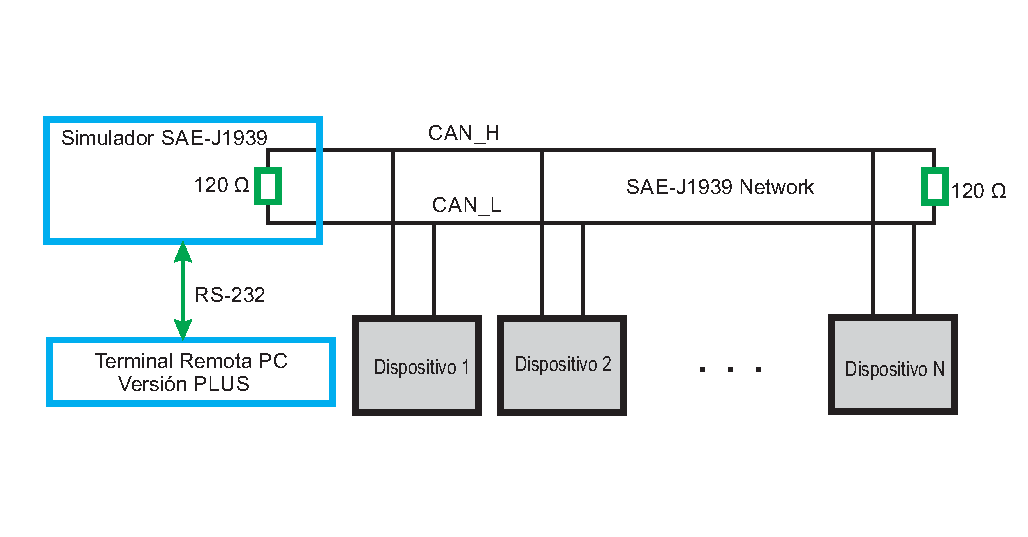
\includegraphics[width=0.8\textwidth]{./Cap6imagen/EjemploSimulador.pdf}
	\caption[Topología de Red SAE J1939.]{Topología de Red SAE J1939.\textbf{ Fuente:} \cite{UserM}.}
	\label{TPSAE} % Etiqueta para la referencia.
\end{figure}



\begin{figure}[H]
	\centering
		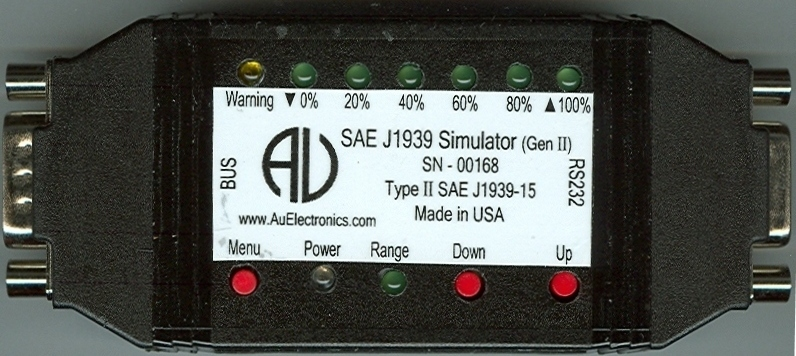
\includegraphics[width=0.8\textwidth]{./Cap6imagen/Simulador.png}
	\caption[Simulador BUS CAN SAE J1939.]{Simulador BUS CAN SAE J1939.\textbf{ Fuente:} \cite{UserM}.}
	\label{Sim} % Etiqueta para la referencia.
\end{figure}


\subsection {Principales Características del Simulador}
El simulador SAE J1939  está equipado con una resistencia de carga interna de 120 ohmios, Protección TVS(\textit{Transient Voltage Suppressor}, por sus siglas en inglés) para protección contra altos niveles de tensión, LED de encendidos, zumbador para indicar el funcionamiento y botones de configuración. 
El simulador tiene como entrada un conector DB9  para las conexiones CANH y CANL, además de la propia alimentación del dispositivo. 
Trabaja a 12V y puede consumir una corriente máxima de 250mA. 
Puede operar en dos modos llamados estáticos y dinámicos. 


\subsection{Modo de Funcionamiento}

Las simulaciones pueden ser operadas con sólo el control de los 3 botones presentes en el equipo. Con la configuración guiada por estos botones se genera una señal SAE J1939 para su uso en desarrollos de sistemas BUS CAN para camiones.

El equipo debe conectarse a una fuente externa entre 9-12 V. 
La alimentación se realiza con los pines 1 (Tierra) y 5 (Potencial positivo), la conexión del BUS CAN tanto CANH como CANL se realiza en los pines 6 y 7 como se muestra en la \textbf{Figura \ref{DB9}}.  
El indicador LED de encendido se ilumina y al estar listo el equipo emite un sonido a través del zumbador, entonces el simulador Au SAE J1939 empieza a funcionar en el modo (estático o dinámico) guardado en la última vez de su funcionamiento.

\begin{figure}[H]
	\centering
		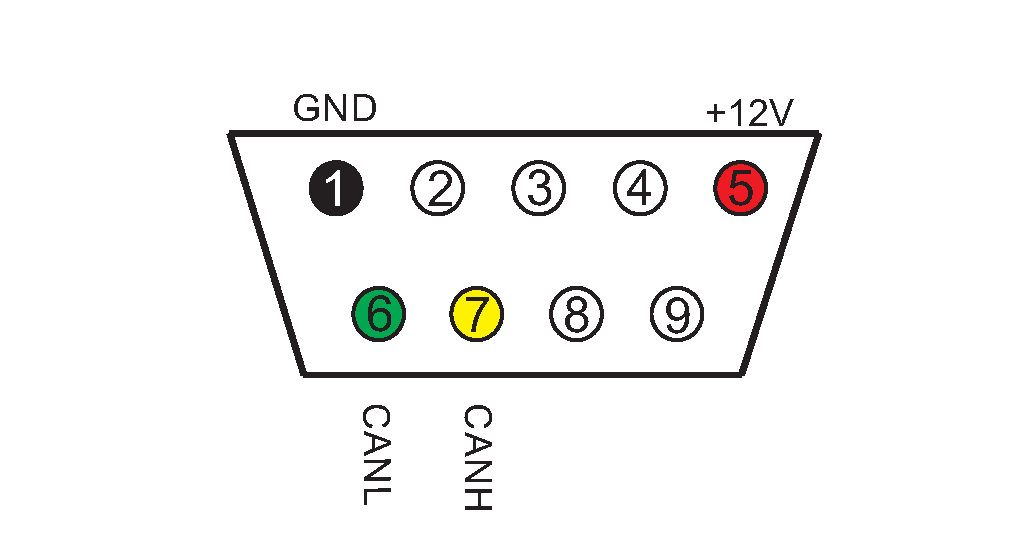
\includegraphics[width=0.8\textwidth]{./Cap6imagen/SimDb9.pdf}
	\caption[Conector DB9 macho BUS CAN.]{Conector DB9 macho BUS CAN.\textbf{ Fuente:} \cite{UserM}.}
	\label{DB9} % Etiqueta para la referencia.
\end{figure}

El modo estático genera una señal SAE J1939 constante, los  dos pulsadores (Up y Down) se utiliza para cambiar las salidas de datos mediante la decisión del usuario. 
En el modo dinámico todos los datos SAE-J1939 cambian automáticamente sin que el rango de valores sea intervenido por el usuario del equipo. 
Para pasar de un modo de funcionamiento a otro se presiona los botones MENU y UP al mismo tiempo durante más de 1 segundo, es decir, para cambiar entre el modo dinámico y el modo estático. 
Una vez realizado, la confirmación del cambio se detecta con un zumbido del equipo.

En el modo estático el botón Down se utiliza para decrementar los valores de las señales SAE-J1939 presentes en las salidas del BUS CAN. 
Los LEDs muestran el descenso de las señales de manera porcentual, de la misma manera el botón Up se utiliza para aumentar los valores de las señales SAE-J1939 y los LEDs muestran el aumento de las señales de manera porcentual. 
la manera de cambiar entre estos dos modos se realiza presionando al mismo tiempo los botones MENÚ y UP por más de un segundo, de esta manera se intercala entre los modos de funcionamiento estático y dinámico. 
Un pitido largo será oído para reflejar la entrada de la tecla MENU y UP.

A modo de resumen se indica las funciones básicas de los botones:
\begin{itemize}
\item Botón DOWN: permite disminuir todos los datos simulados hasta que alcanza el valor más bajo.
 \item botón UP: permite aumentar todos los datos simulados hasta que alcanza el valor más alto.
\item MENÚ + UP: Cambia el funcionamiento del simulador entre el modo estático y dinámico.

\end{itemize}

\section{Pruebas Realizadas con el Simulador J1939}
Se realiza una prueba con el simulador y para ello conectamos un bus entre el hardware y el simulador J1939, alimentados ambos por una fuente de tensión de 12v. Como se observa en la Figura~\ref{simulador_ref_c6}

\begin{figure}[H]
	\centering
	\includegraphics[width=0.5\textwidth]{./Cap6imagen/simulador_fig_c6.jpg}
	\caption [Conexión del Simulador J1939.]{Conexión del Simulador J1939 \textbf{ Fuente:} %\cite{cite_can_c3}.}
		Elaboración propia.}
	\label{simulador_ref_c6} % Etiqueta para la referencia.
\end{figure}

Se conecta el modulo Xbee receptor al puerto USB de la computadora y se inicia el software al acceder en la página web, Figura~\ref{receptor_ref_c6},  se selecciona el sistema J1939 y con el botón escucha se va recibiendo los datos enviados. 


\begin{figure}[H]
	\centering
	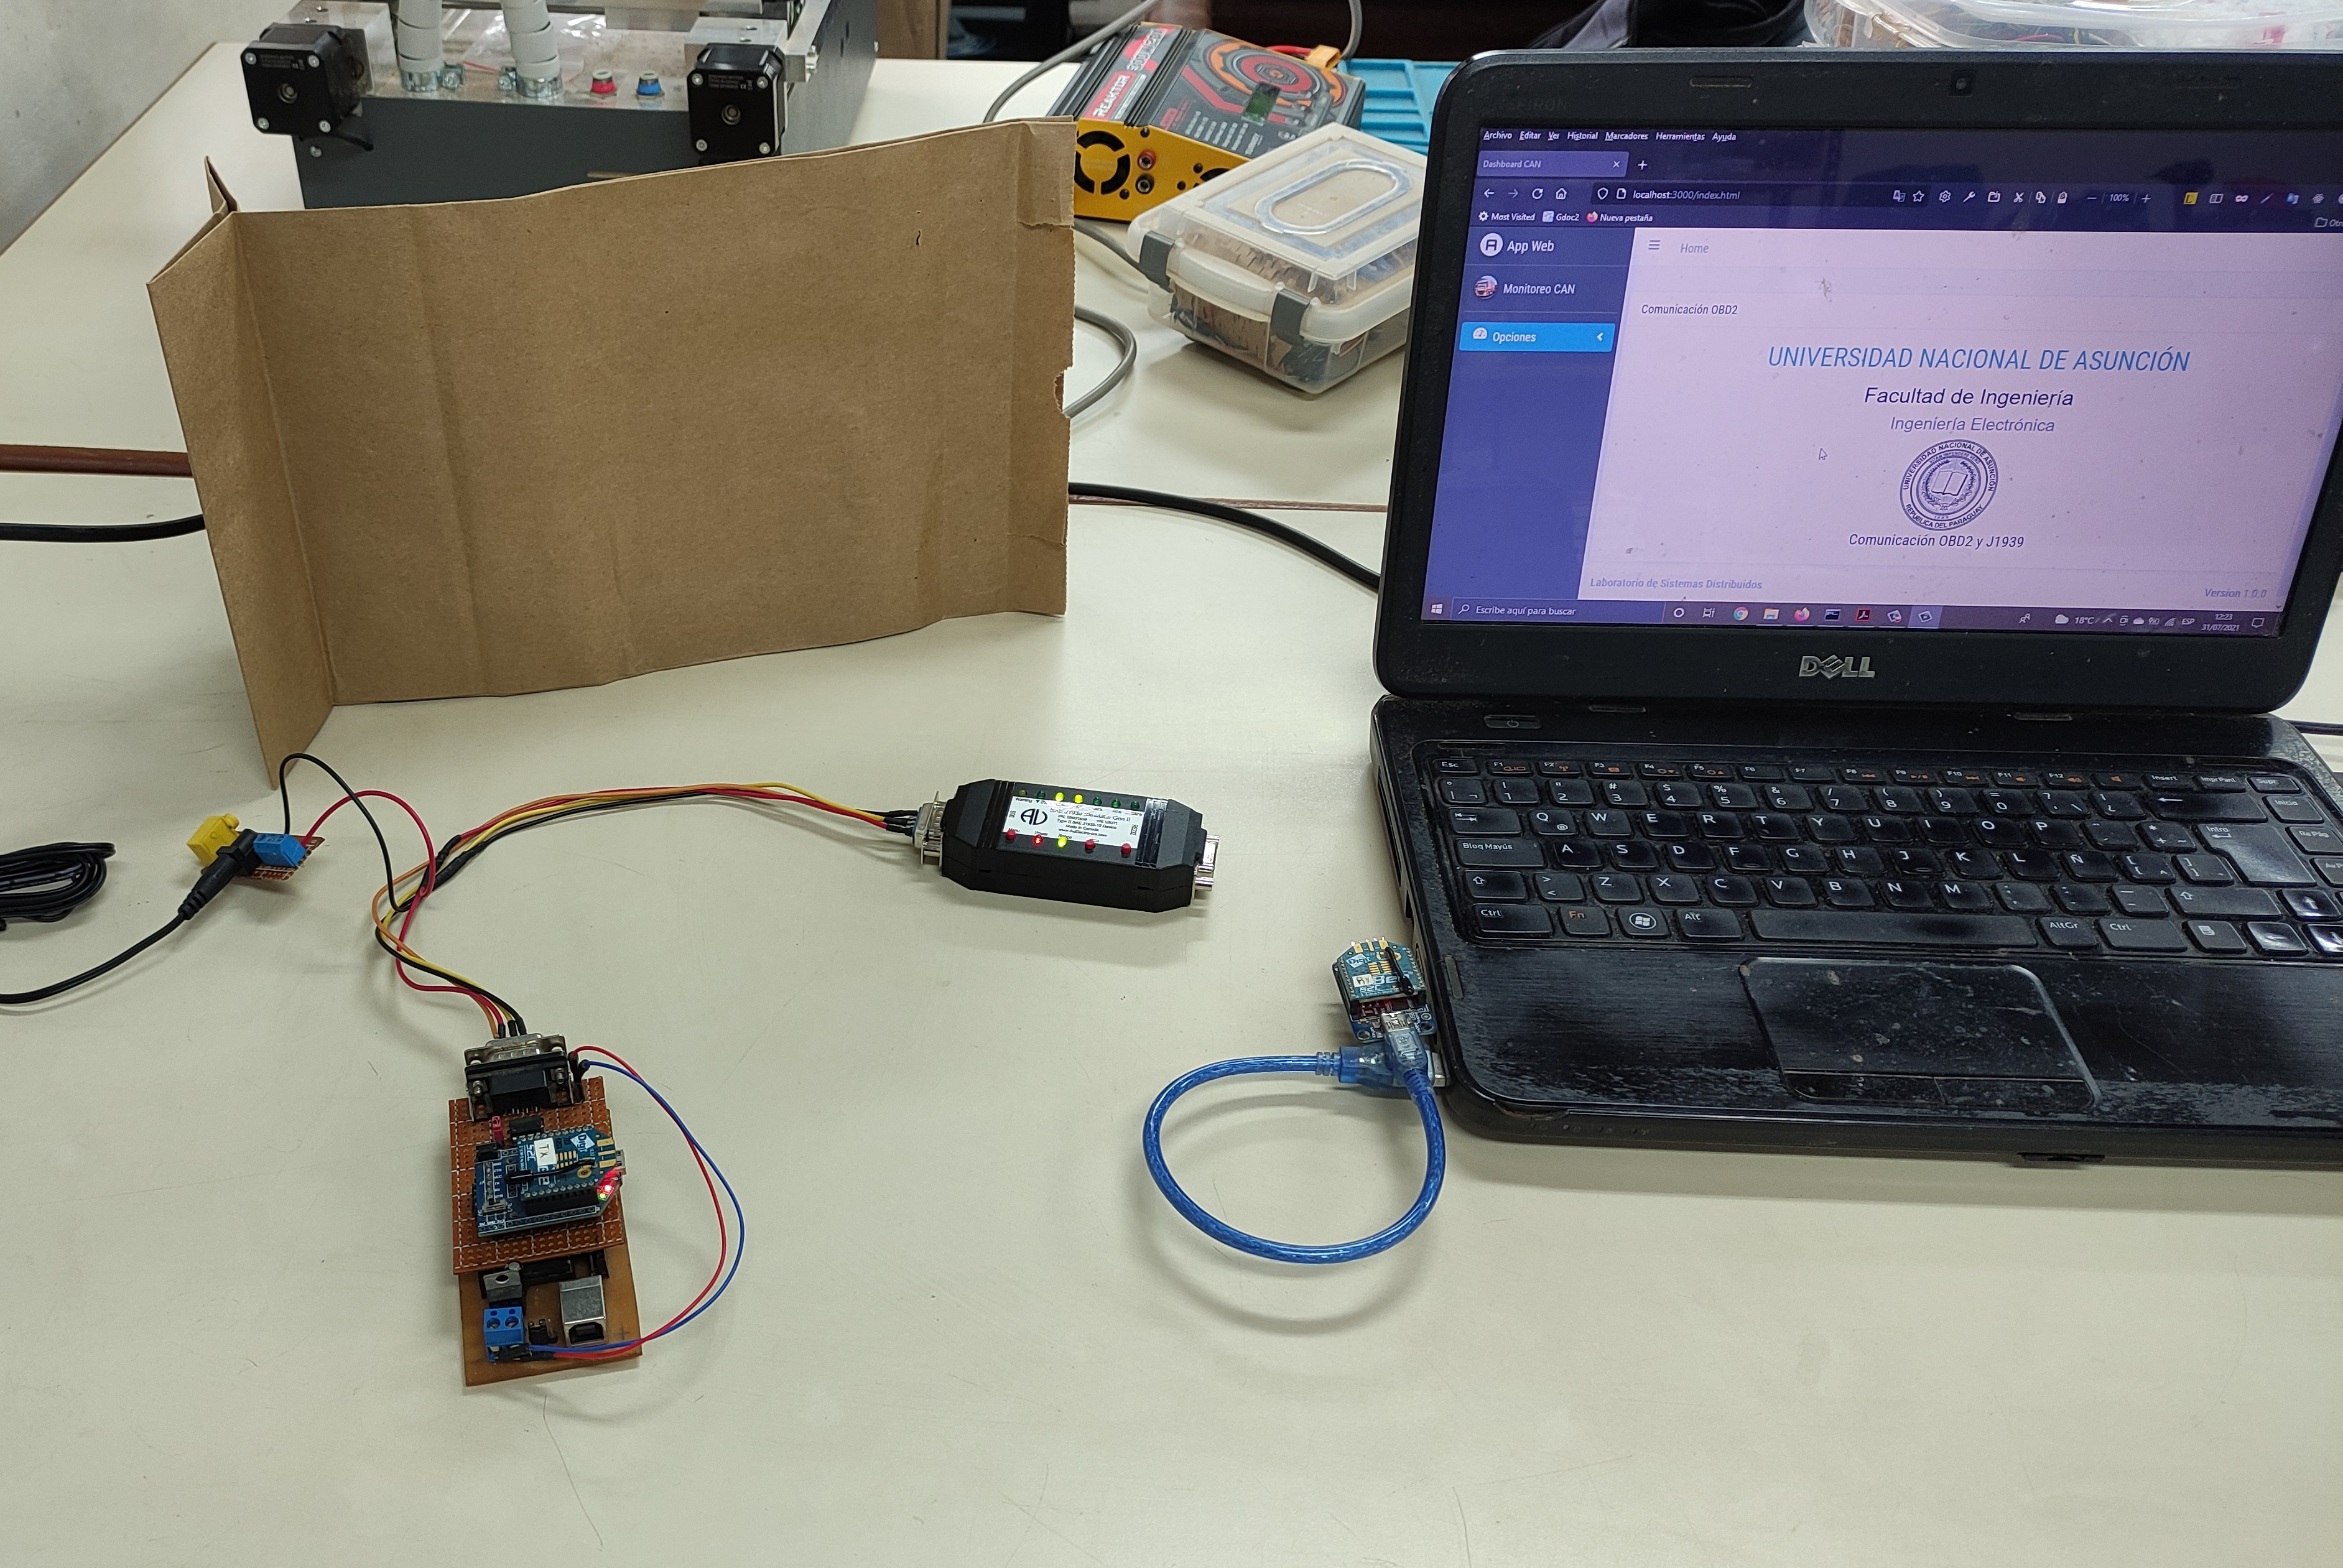
\includegraphics[width=0.5\textwidth]{./Cap6imagen/receptor_fig_c6.jpg}
	\caption [Receptor ubicado en el puerto USB.]{Receptor ubicado en el puerto USB \textbf{ Fuente:} %\cite{cite_can_c3}.}
		Elaboración propia.}
	\label{receptor_ref_c6} % Etiqueta para la referencia.
\end{figure}

Se selecciona la opción datos y observamos todas las tramas J1939 que está presente en el bus, aquí se puede observar la dirección de destino y origen de los dispositivos, los 8 bytes de datos en el cual los valores FF significa que dichos datos no están disponibles, pero los demás datos distintos a FF significan que son datos reales y disponibles, también podemos observar la prioridad de los mensajes que varía entre 3 y 6 según la Figura \ref{escucha_ref_c6}.

\begin{figure}[H]
	\centering
	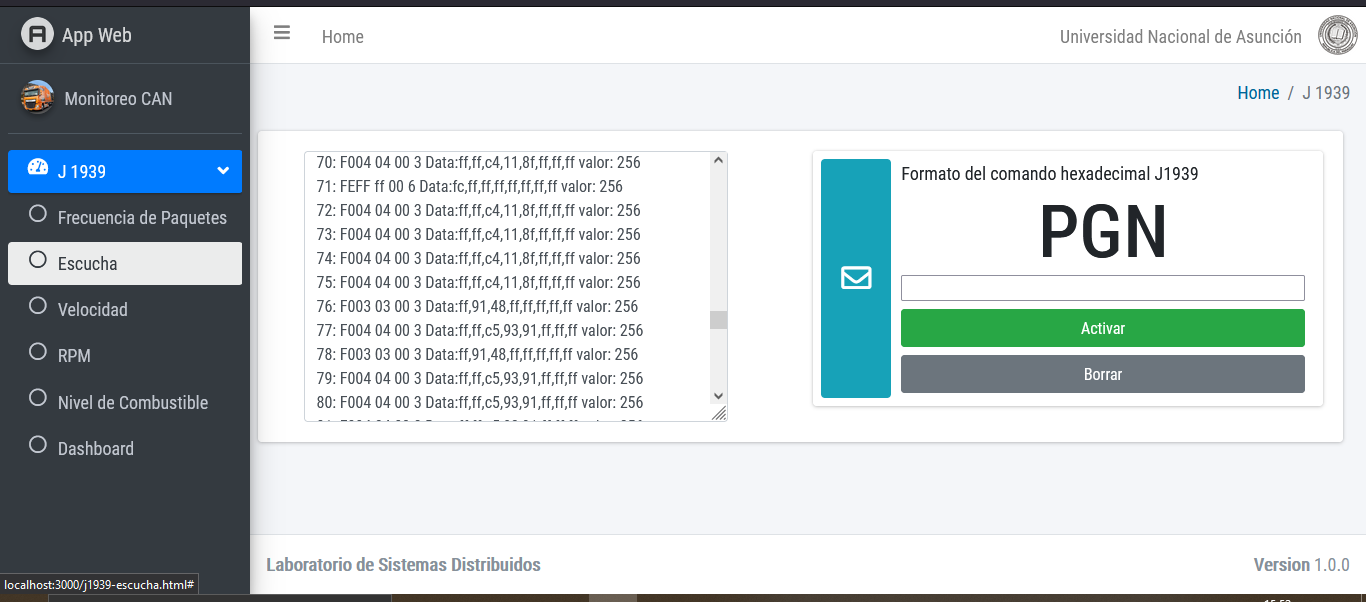
\includegraphics[width=0.8\textwidth]{./Cap6imagen/escucha_fig_c6.png}
	\caption [Datos leídos del BUS CAN J1939.]{Datos leídos del BUS CAN J1939 \textbf{ Fuente:} %\cite{cite_can_c3}.}
		Elaboración propia.}
	\label{escucha_ref_c6} % Etiqueta para la referencia.
\end{figure}


También se puede observar la frecuencia de tipos de paquetes CAN presentes en el bus, en la Figura~\ref{paquetes_ref_c6}, los paquetes 0xF004 han sido recibidos 102 veces y los paquetes 0xFEF2 solamente 2 veces han sido captados. 
Hay varias tramas CAN que el simulador nos envía y mientras van apareciendo, el hardware los va captando y a su vez enviando al computador para su visualización. 
En el caso de la 


\begin{figure}[H]
	\centering
	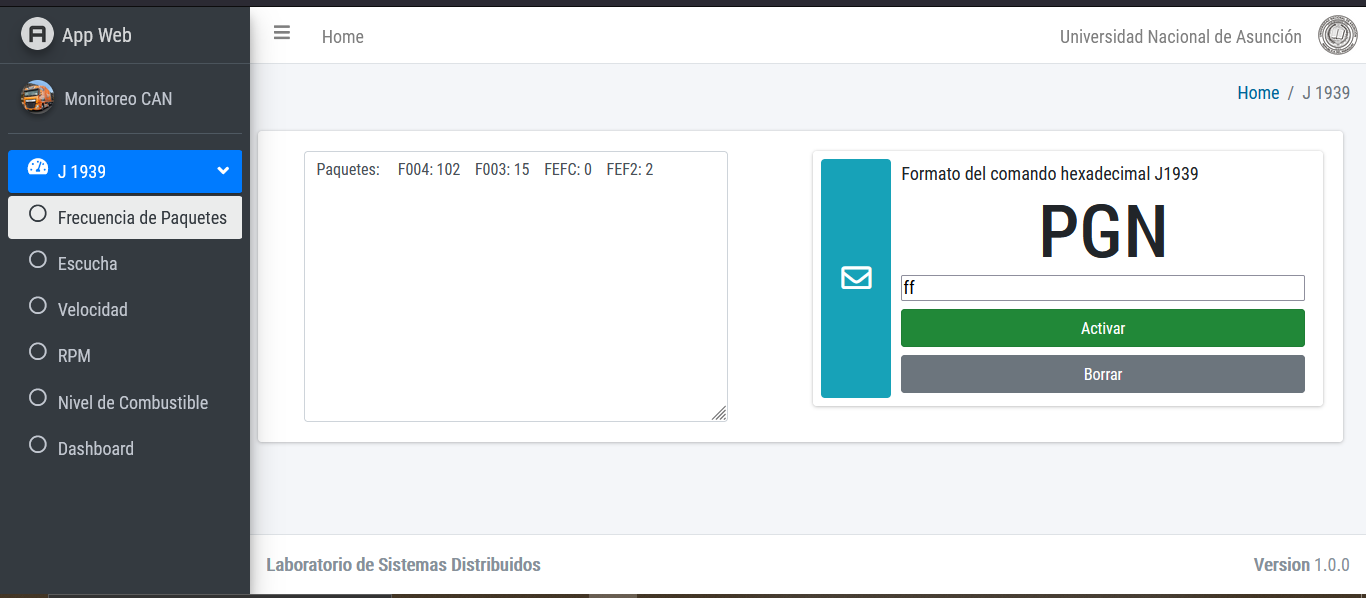
\includegraphics[width=0.8\textwidth]{./Cap6imagen/paquetes_fig_c6.png}
	\caption [Tramas CAN J1939 presentes.]{Tramas CAN J1939 presentes \textbf{ Fuente:} %\cite{cite_can_c3}.}
		Elaboración propia.}
	\label{paquetes_ref_c6} % Etiqueta para la referencia.
\end{figure}


En la Figura~\ref{real_ref_c6} siguiente podemos observar la distribución de los datos aleatorios que van dejando el simulador en el bus, en este caso pertenece a la velocidad del vehículo. 
Se puede ver la forma en la cual el simulador distribuye los datos con el tiempo.  
Los datos van ingresando y el programa ajusta la gráfica para que quepan todos los datos y se pueda observar su comportamiento.  

\begin{figure}[H]
	\centering
	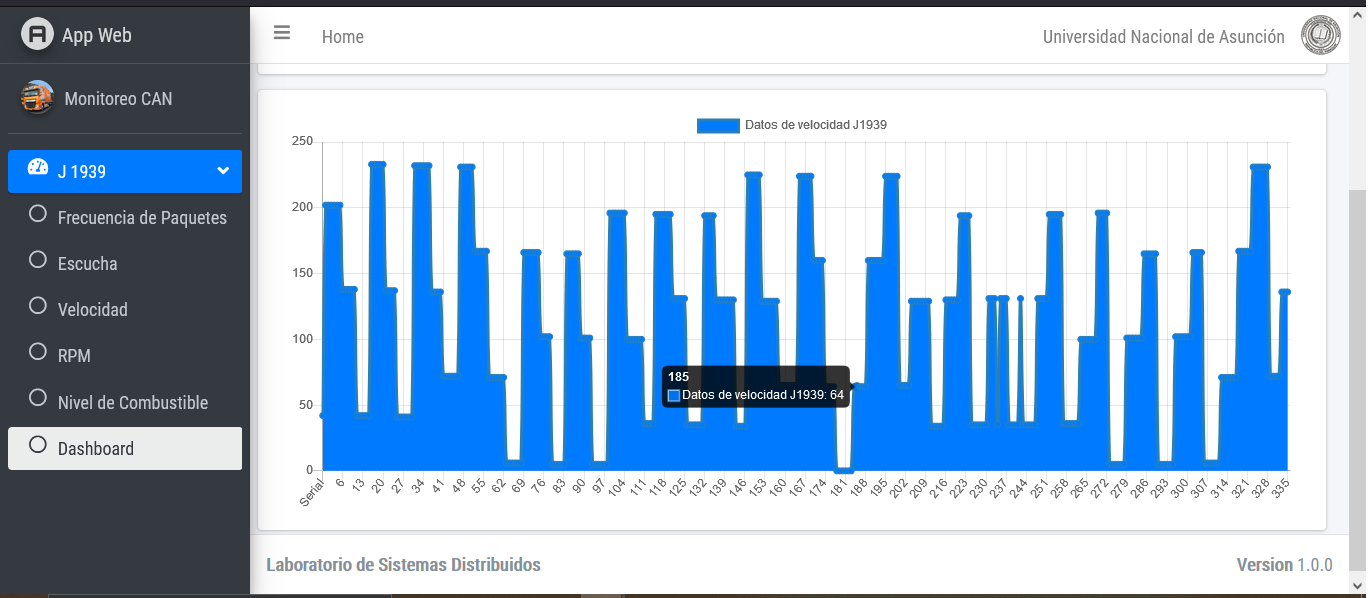
\includegraphics[width=0.8\textwidth]{./Cap6imagen/real_fig_c6.png}
	\caption [Datos de Velocidad del BUS CAN J1939.]{Datos de velocidad del BUS CAN J1939 \textbf{ Fuente:} %\cite{cite_can_c3}.}
		Elaboración propia.}
	\label{real_ref_c6} % Etiqueta para la referencia.
\end{figure}


En la Figura \ref{gauge_ref_c6} observamos una visualización en formato de tablero, para visualizar los datos manera familiar a la de un tablero de vehículo. 
Para obtenerlo, presionamos velocidad y luego activar, para poder filtrar de entre todas las tramas la trama que contiene los datos de la velocidad, se observa una captura de velocidad de 158 metros por segundo. 


\begin{figure}[H]
	\centering
	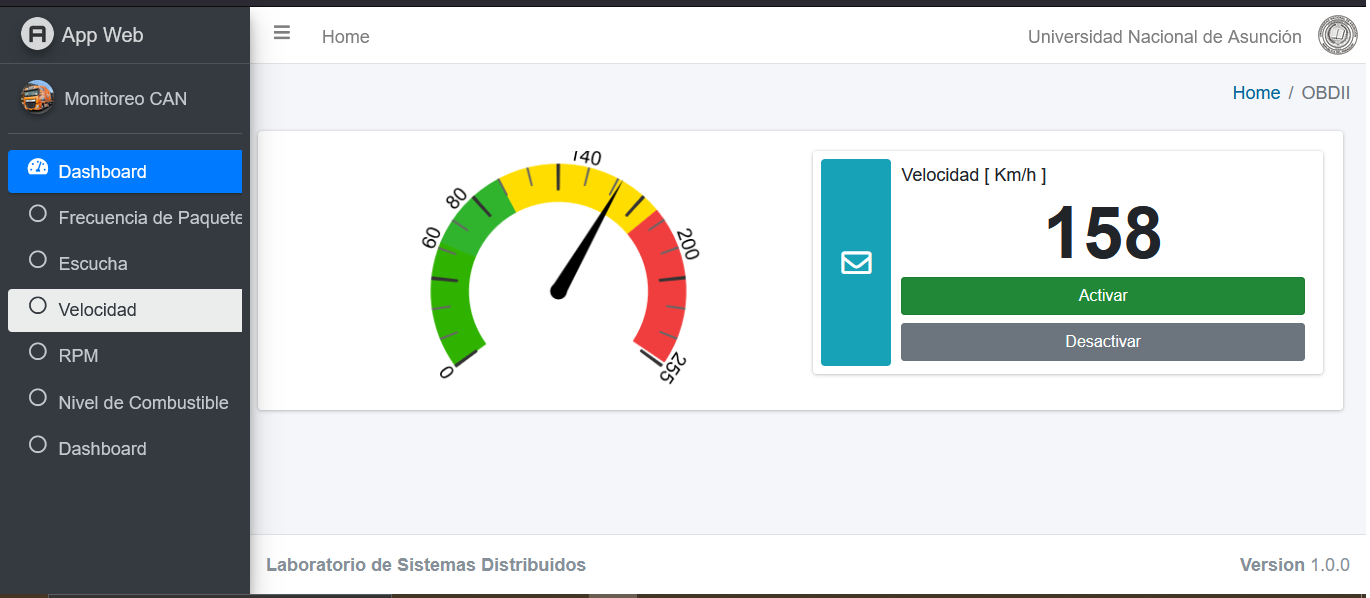
\includegraphics[width=0.8\textwidth]{./Cap6imagen/gauge_fig_c6.png}
	\caption [Tablero de Velocidad J1939.]{Tablero de velocidad J1939 \textbf{ Fuente:} %\cite{cite_can_c3}.}
		Elaboración propia.}
	\label{gauge_ref_c6} % Etiqueta para la referencia.
\end{figure}

\section{Pruebas realizadas en Vehículos con el sistema OBD II}

Para el sistema OBD II fue puesta a prueba el sistema en tres vehículos de las marcas Toyota 2019, Hyundai Creta 2021 y Hyundai Tucson 2011, en donde se realizó las medidas de distintos sensores para obtener datos de revoluciones por minuto del motor, voltaje de batería, velocidad y lectura de lista de sensores presentes en el vehículo,etc. 
Se puede ver en las Figuras \ref{auto_ref_c6}, \ref{creta_ref_c6} y \ref{tucson_ref_c6}  las imágenes de los tipos de vehículo automotor usados en las pruebas. 

\begin{figure}[H]
	\centering
	\includegraphics[width=0.8\textwidth]{./Cap6imagen/auto_fig_c6.jpg}
	\caption [Vehículo utilizado para la Prueba OBD II.]{Vehículo utilizado para la Prueba OBD II \textbf{ Fuente:} %\cite{cite_can_c3}.}
		Elaboración propia.}
	\label{auto_ref_c6} % Etiqueta para la referencia.
\end{figure}

\begin{figure}[H]
	\centering
	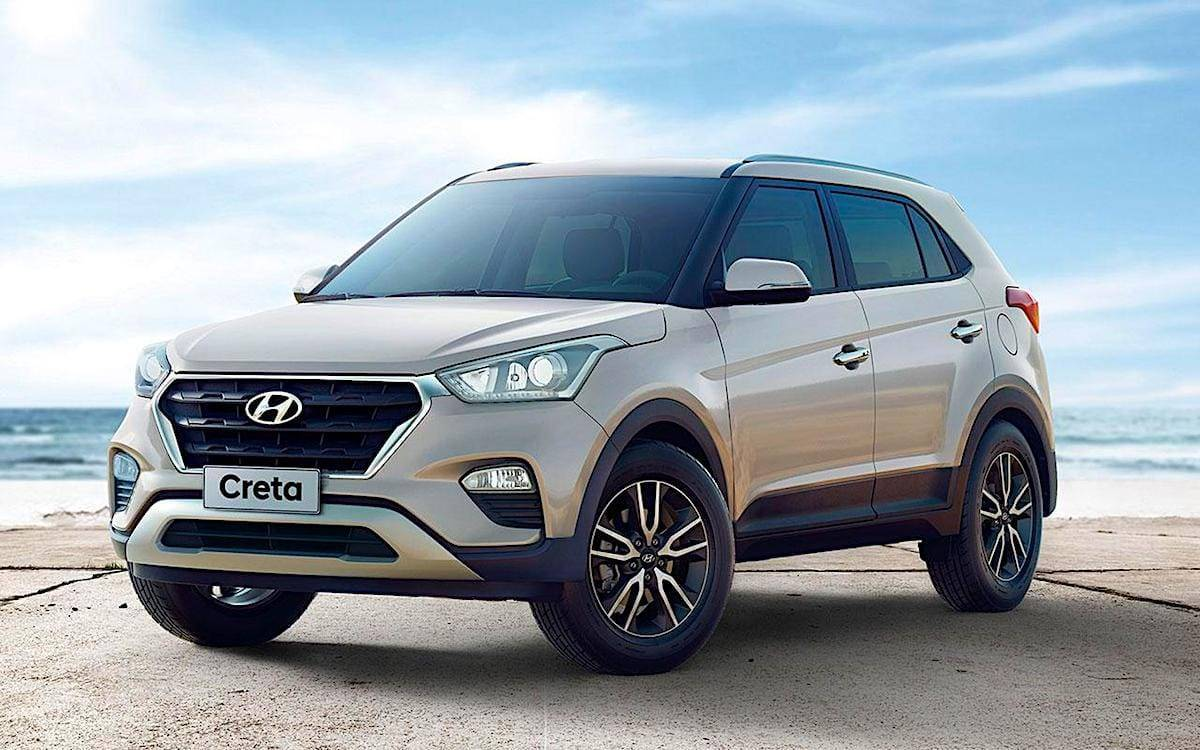
\includegraphics[width=0.8\textwidth]{./Cap6imagen/creta_fig_c6.jpg}
	\caption [Vehículo Creta 2021 utilizado para la Prueba OBD II.]{Vehículo Creta 2021 utilizado para la Prueba OBD II \textbf{ Fuente:} %\cite{cite_can_c3}.}
		Elaboración propia.}
	\label{creta_ref_c6} % Etiqueta para la referencia.
\end{figure}

\begin{figure}[H]
	\centering
	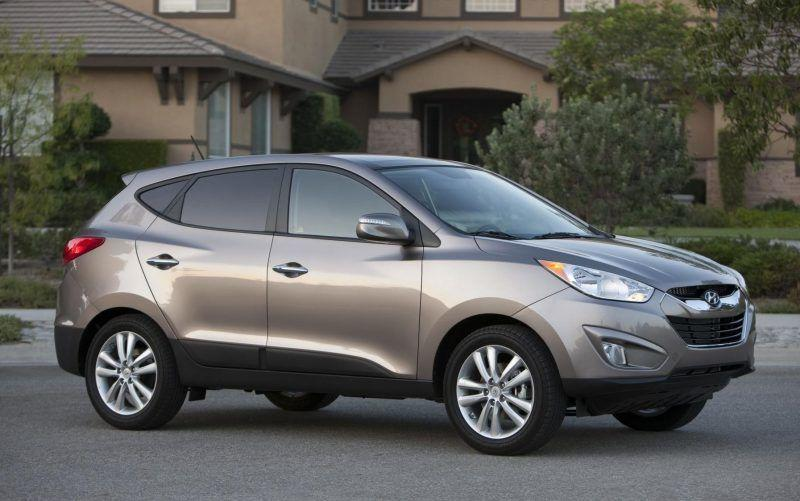
\includegraphics[width=0.8\textwidth]{./Cap6imagen/tucson_fig_c6.jpg}
	\caption [Vehículo Tucson 2011 utilizado para la Prueba OBD II.]{Vehículo Tucson 2011 utilizado para la Prueba OBD II \textbf{ Fuente:} %\cite{cite_can_c3}.}
		Elaboración propia.}
	\label{tucson_ref_c6} % Etiqueta para la referencia.
\end{figure}

En la Figura\ref{panel_ref_c6} observamos las consultas soportadas actualmente por el sistema, que son:
\begin{itemize}
    \item \textbf{Soportes PIDs}: presenta la lista de sensores del vehículo. 
    \item \textbf{Consulta PID}: sirve para consultar sensores que no soporta el sistema de visualización pero podemos leer la codificación. 
    \item \textbf{Revoluciones}: sirve para visualizar las revoluciones por minuto del motor vehicular.
    \item \textbf{Batería, Temperatura y velocidad} son otras visualizaciones soportadas.     
\end{itemize}



\begin{figure}[H]
	\centering
	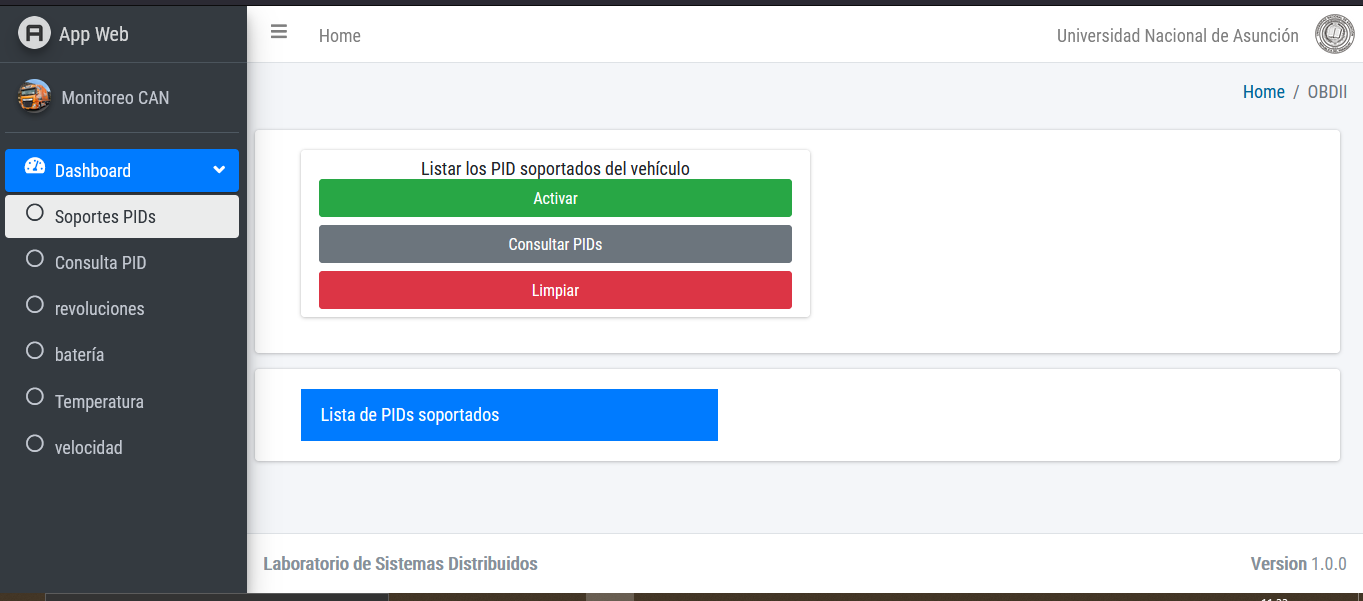
\includegraphics[width=0.8\textwidth]{./Cap6imagen/soportes_fig_c6.png}
	\caption [Panel Principal OBD II.]{Panel Principal OBD II \textbf{ Fuente:} %\cite{cite_can_c3}.}
		Elaboración propia.}
	\label{panel_ref_c6} % Etiqueta para la referencia.
\end{figure}


En la Figura\ref{consola_ref_c6} se pueden ver en modo consola las lecturas de algunos sensores del vehículo Toyota como las revoluciones por minuto, velocidad, niveles de batería y otros. 
Para el momento de la captura de imagen el sistema indicaba mediciones de rpm (revoluciones por minuto) del motor. 

\begin{figure}[H]
	\centering
	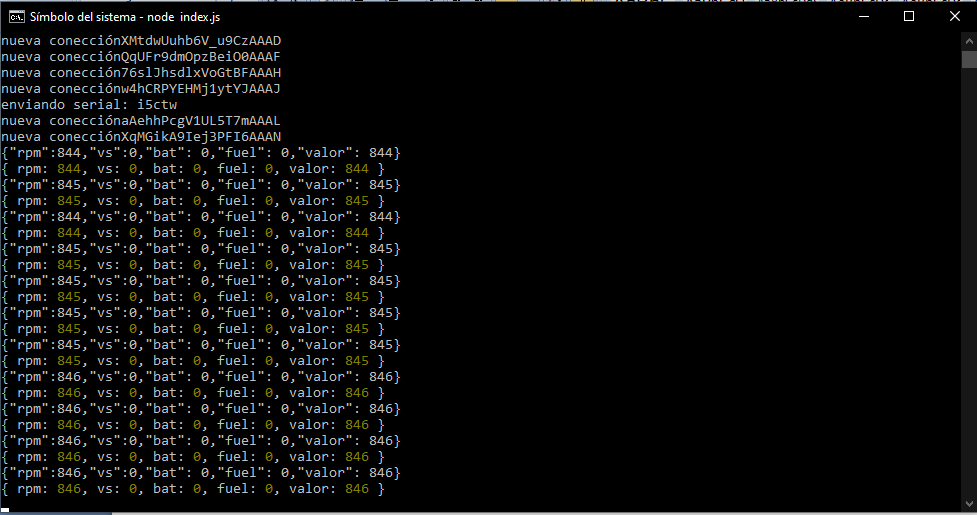
\includegraphics[width=0.8\textwidth]{./Cap6imagen/consola_fig_c6.png}
	\caption [Datos recibidos del Vehículo.]{Datos recibidos del Vehículo \textbf{ Fuente:} %\cite{cite_can_c3}.}
		Elaboración propia.}
	\label{consola_ref_c6} % Etiqueta para la referencia.
\end{figure}


 Se realizó una lectura de medición de temperatura del aceite de motor en reposo, es decir, antes de arrancar el motor del vehículo, se observó la siguiente medición que se muestra en la Figura \ref{temp_ref_c6}. 
 La medida fue de 38 grados Celsius, la misma se presenta con un termómetro animado del lado izquierdo y el valor numérico del lado derecho.
 
 \begin{figure}[H]
	\centering
	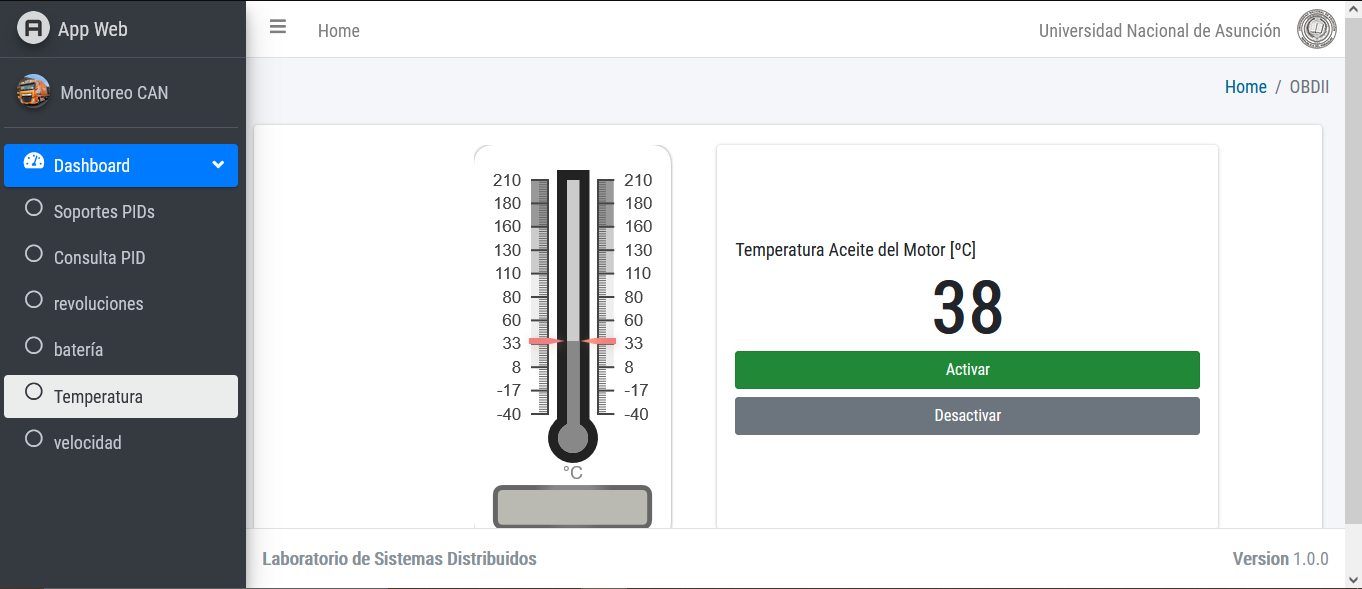
\includegraphics[width=0.8\textwidth]{./Cap6imagen/temp_fig_c6.png}
	\caption [Visualización de la medida del sensor de temperatura de aceite del motor en reposo.]{Visualización de la medida del sensor de temperatura de aceite del motor en reposo \textbf{ Fuente:} %\cite{cite_can_c3}.}
		Elaboración propia.}
	\label{temp_ref_c6} % Etiqueta para la referencia.
\end{figure}

Otra medida de prueba fueron las revoluciones por minuto en estado de reposo, pero con el vehículo encendido, se observa en la Figura~\ref{rpm_ref_c6} la lectura obtenida de 872 rpm del motor del vehículo, nuevamente en dos formatos para una lectura familiarizada con el tablero analógico de un vehículo y otra digitalmente. 

\begin{figure}[H]
	\centering
	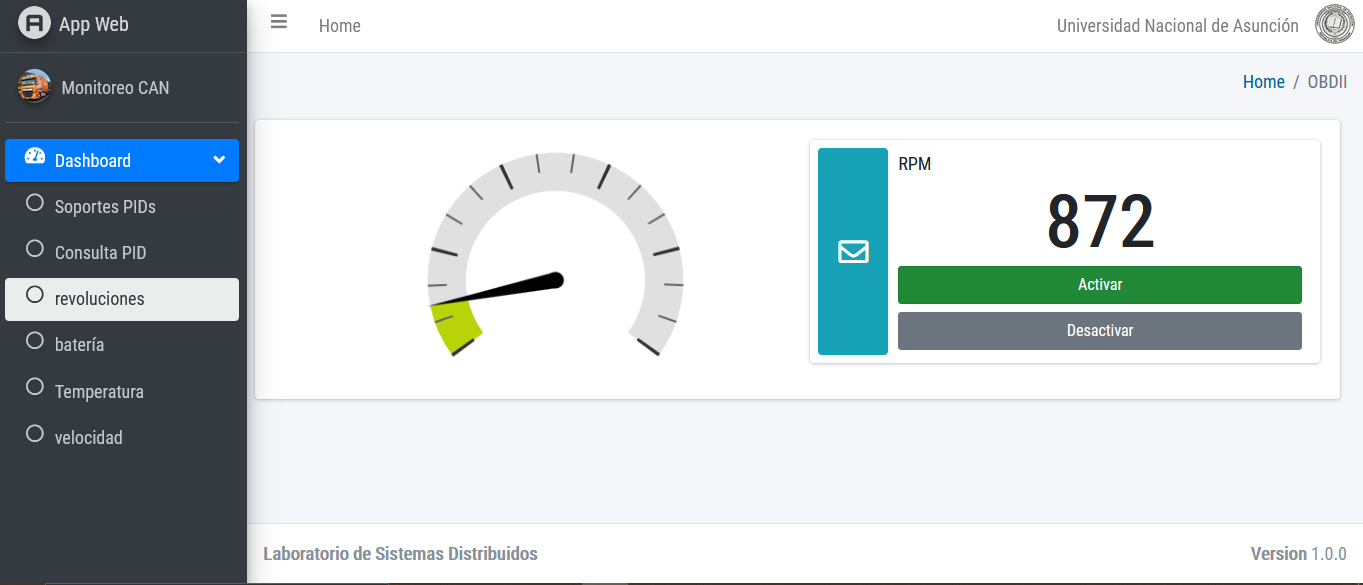
\includegraphics[width=0.8\textwidth]{./Cap6imagen/rpm_fig_c6.png}
	\caption [Visualización de la medida del sensor de revoluciones por minuto con el motor en reposo.]{Visualización de la medida del sensor de revoluciones por minuto con el motor en reposo.  \textbf{ Fuente:} %\cite{cite_can_c3}.}
		Elaboración propia.}
	\label{rpm_ref_c6} % Etiqueta para la referencia.
\end{figure}


Para el vehículo modelo \textbf{Tucson 2011} se realizaron las pruebas de: 


\begin{itemize}
    \item Lista de algunos sensores presentes en el vehículo
    \item Sensor de velocidad
    \item Voltaje de Batería en contacto marca una tensión de 12V y una vez encendido el motor marca una tensión de 14V, con lo cuál se puede concluir que son lecturas coherentes, pues el generador está activo y recargando la batería del vehículo. 
    \item Medida de revoluciones por minuto del motor en estado de reposo. 
    \item tiempo de encendido del motor
\end{itemize}

Algunas de estas  mediciones se muestran en la Figura \ref{dash_ref_c6}, además de una muestra por consola de los datos recibidos del hardware. 

\begin{figure}[H]
	\centering
	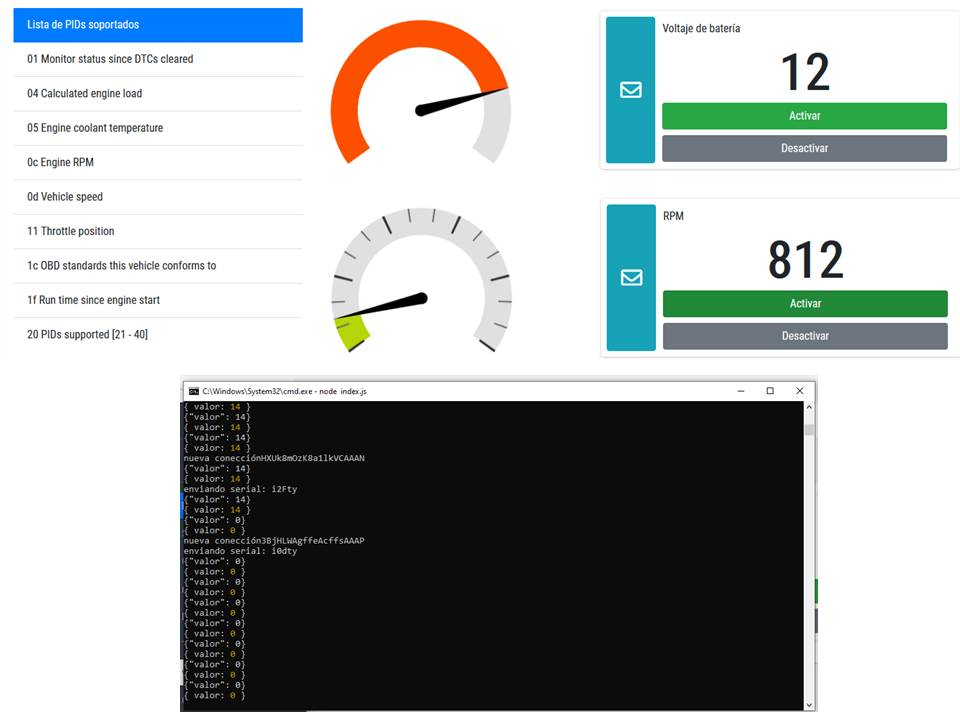
\includegraphics[width=0.8\textwidth]{./Cap6imagen/dash_fig_c6.jpg}
	\caption [Visualización de varias medidas de sensores.]{Visualización de varias medidas de sensores.  \textbf{ Fuente:} %\cite{cite_can_c3}.}
		Elaboración propia.}
	\label{dash_ref_c6} % Etiqueta para la referencia.
\end{figure}


El sistema provee una manera de leer los sensores que el hardware no tiene programado para hacerlo. 
Esto se realiza enviando el código PID deseado y  se traslada el calculo de la trama CAN al cliente. 
Para el ejemplo se realiza la lectura del temporizador del vehículo, el cual nos indica el tiempo que lleva encendido el automotor. 
Para ello se consulta el documento SAE J1979, se observa el código PID y la formula requerida de lectura del temporizador. 
Estos datos se introducen en el sistema mediante la interfaz gráfica, Figura~\ref{consulta_ref_c6}, una vez presionado el botón \"activar\", el software dibuja  una gráfica en el tiempo de los valores de la consulta. 
En la Figura~\ref{grafica_ref_c6} se observa la lectura del temporizador en el tiempo indicando que el automóvil lleva encendido 650 segundos. 

\begin{figure}[H]
	\centering
	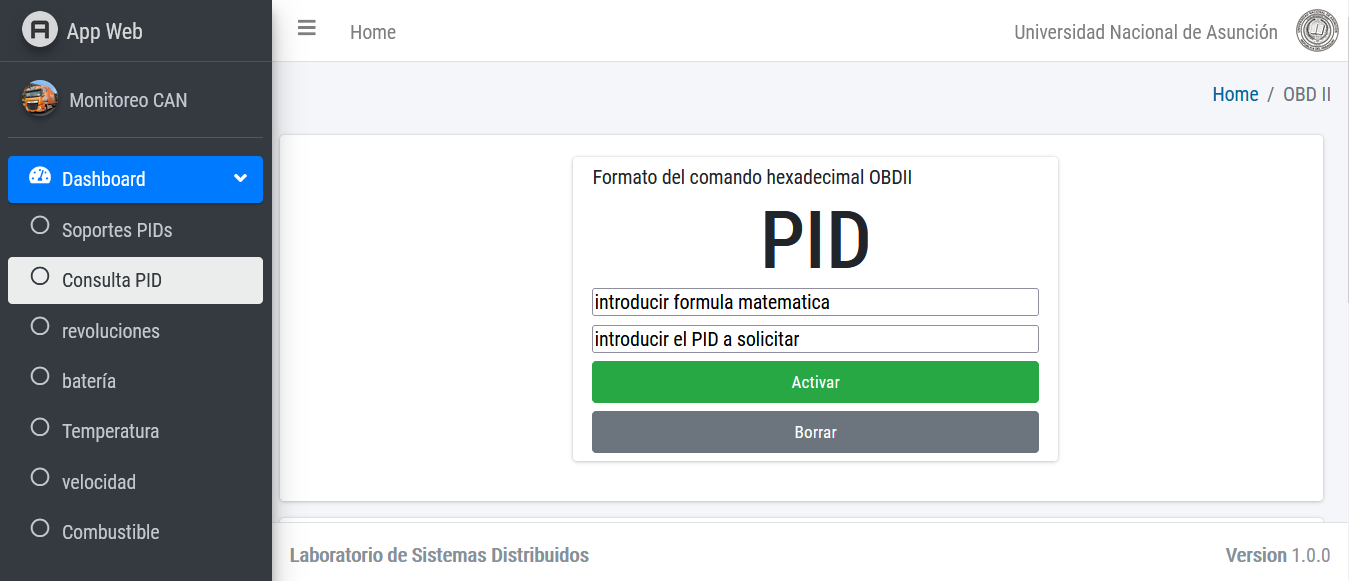
\includegraphics[width=0.8\textwidth]{./Cap6imagen/consulta_fig_c6.png}
	\caption [Visualización de varias medidas de sensores.]{Visualización de varias medidas de sensores.  \textbf{ Fuente:} %\cite{cite_can_c3}.}
		Elaboración propia.}
	\label{consulta_ref_c6} % Etiqueta para la referencia.
\end{figure}

\begin{figure}[H]
	\centering
	\includegraphics[width=0.8\textwidth]{./Cap6imagen/grafica_fig_c6.jpg}
	\caption [Visualización de varias medidas de sensores.]{Visualización de varias medidas de sensores.  \textbf{ Fuente:} %\cite{cite_can_c3}.}
		Elaboración propia.}
	\label{grafica_ref_c6} % Etiqueta para la referencia.
\end{figure}

Para el automotor modelo Creta 2021 además de leer los mismos datos anteriores, se realizó una prueba en movimiento para medir los datos de los sensores de velocidad. 
La lectura se visualiza en la Figura \ref{vel_ref_c6} en dónde se compara con el tablero del vehículo.

\begin{figure}[H]
	\centering
	\includegraphics[width=0.9\textwidth]{./Cap6imagen/vel_fig_c6.png}
	\caption [Comparación de la medida de Velocidad en un vehículo Creta 2021.]{Comparación de la medida de Velocidad en un vehículo Creta 2021.  \textbf{ Fuente:} %\cite{cite_can_c3}.}
		Elaboración propia.}
	\label{vel_ref_c6} % Etiqueta para la referencia.
\end{figure}

Con estas pruebas se lograron la lectura de los sensores básicos presentes en los vehículos. 

\section{Inconvenientes encontrados en las Pruebas}

Durante las pruebas han sido necesario ajustar algunos parámetros y se ha encontrado otras dificultades enunciadas a continuación: 
\begin{itemize}
    \item Ha sido necesario ajustar el bit denominado RTR en el módulo del protocolo CAN, cuyo valor estándar es 1 (uno) y tuvo que ser cambiado a 0 (cero) para la comunicación. El bit RTR es el encargado de solicitar una trama CAN a los dispositivos en la red, se observó que los estándares J1939 y OBD-II no implementan el bit RTR, por lo que se ajustó su valor a cero. 
    
    \item La mayoría de los autos presentaban fallas de comunicación por avería del conector OBD-II o el propio sistema. Esto se comprobó con un escáner vehicular comercial. 
    
    \item Algunos automóviles  no contaban con el protocolo CAN, sino con otros tipos de protocolos, como la ISO 14230-4 KWP. No todos los vehículos  implementan el protocolo CAN actualmente. 
    
\end{itemize}


El escáner vehicular utilizado para la comprobación  y comparación del funcionamiento del sistema CAN desarrollado se muestra en la Figura~\ref{scaner_fig_c6}: 

\begin{figure}[H]
	\centering
	\includegraphics[width=0.6\textwidth]{./Cap6imagen/scaner_fig_c6.png}
	\caption [Escáner de la Marca Launch CRP123.]{Escáner de la Marca Launch CRP123.  \textbf{ Fuente:} %\cite{cite_can_c3}.}
		Elaboración propia.}
	\label{scaner_fig_c6} % Etiqueta para la referencia.
\end{figure}

\section[Análisis Financiero]{Análisis Financiero}

\subsection{Costos del Hardware y Software desarrollados}
En el proyecto se analizaron los gastos teniendo en cuenta  recursos materiales y humanos utilizados. 
Para el calcular el proceso de esfuerzo humano se realizó un promedio del salario en base a un desarrollador de software en Paraguay. 
Como el proyecto está hecho con lenguajes de programación web para el software y lenguaje C para el hardware se vio que los Desarrolladores web y multimedia ganan normalmente un salario neto mensual aproximado de entre Gs. 3.000.000 y Gs. 6.000.000 al empezar en el puesto de trabajo, esto según las referencias obtenidas de la página tusalario.org,~\cite{tusalario}, así haciendo un promedio y suponiendo 20 días de trabajo al mes con 8 horas diarias, el costo por horas de trabajo es de 30 000Gs por hora aproximadamente. 
Se aborda este salario para el trabajo en \textit{backend}, \textit{frontend}, desarrollo de hardware y su programación. 
Como no se trabaja las 8 horas diarias por el desarrollo del sistema, empleamos 4 horas diarias para el desarrollo y las restantes 4 horas para otras gestiones e investigaciones que no carga con las horas del diseño en sí. 

En la Tabla~\ref{tabla:hw} se observa el costo de los componentes utilizados para el hardware, además de las herramientas utilizadas para su elaboración. 


%%%%%%%%%%%%%%%%%%%%% tabla %%%%%%%%%%%%%%%%%%%%%%%%%%%%%%%%
\begin{table}[H]
\begin{center}
\begin{tabular}{c l l r r }
\toprule
\textbf{Cant} & \textbf{Componente} & \textbf{Descripción} &\textbf{Unidad Gs.}&\textbf{Importe Gs.}  \\ 
\midrule
2    & Capacitores      & 10uF        & 250            & 500   \\ 
%\hline
2    & Capacitores      & 0,1uF       & 250            & 500   \\ 
%\hline
2    & Capacitores      & 15pf        & 1.000           & 2.000  \\ 
%\hline
1    & Resistor         & 330 ohm     & 250            & 250   \\ 
%\hline
1    & Resistor         & 100k        & 250            & 250   \\ 
%\hline
1    & Microcontrolador &PIC18F4580   & 85.000          & 85.000 \\ 
%\hline
1    & Regulador        & 7805        & 15.000          & 15.000 \\ 
%\hline
2    & Diodo            & 1N4148      & 1.000           & 2.000  \\ 
%\hline
1    & Diodo Led        & Rojo        & 1.000           & 1.000  \\ 
%\hline
1    & Botón            & 4 pines    & 3.500           & 3.500  \\ 
%\hline
1    & Conector        & DB9    & 5.000           & 5.000  \\ 
%\hline
1    & Espadines       & 5 pines   & 3.500           & 3500  \\ 
%\hline
2    & Módulo          & SHIELD & 55.000          & 110.000 \\ 
%\hline
2    & Módulo          & XBEE        & 250.000         & 500.000 \\ 
%\hline
2    & Espadines       & 20 pines  & 3.500           & 7.000    \\ 
%\hline
1    & Módulo          & MCP2551     & 30.000          & 30.000  \\ 
%\hline
1    & Cristal         & 16Mhz     & 5.000           & 5.000   \\ 
%\hline
1    & Placa de Cobre  & 1 Capa      & 13.000          & 13.000   \\ 
%\hline
1    & Conector OBD II  & OBD II     & 50.000          & 50.000   \\ 
%\hline
1    & Impresora 3D         & Caja 3D       & 100.000         & 100.000 \\ 
%\hline
1    & Fresadora CNC    & CNC        & 100.000         & 100.000 \\ 
%\hline
      &                  &            & \textbf{Total} & \textbf{1.033.500}  \\ 
      \bottomrule
\end{tabular}
\caption{Costo de los componentes y herramientas usadas en el hardware.}
\label{tabla:hw}
\end{center}
\end{table}

Para el desarrollo del proyecto se organizó el trabajo en 4 partes:  diseño del hardware, programación del hardware, Programación del Software \textit{frontend} (Diseño de Usuario) y Programación del software \textit{backend} (Programación del servidor), cada uno con un costo de 30.000 Gs/hora-hombre y un tiempo total de 1120hs. repartidas en las distintas etapas del desarrollo, como se aprecia en la Tabla~\ref{tabla:software} con sus costos correspondientes. 

%%%%%%%%%%%%%%%%%%%%% tabla %%%%%%%%%%%%%%%%%%%%%%%%%%%%%%%%
\begin{table}[H]
\begin{center}
\begin{tabular}{l r r r}
\toprule
\textbf{Trabajo Realizado} & \textbf{Horas}&\textbf{Salario por hora Gs.} & \textbf{Importe Gs.} \\ \hline

 Placa Electrónica & 160 & 30.000  & 4.800.000     \\ 
 %\hline
 Software CAN      & 320 & 30.000  & 9.600.000     \\ 
 %\hline
 Diseño de Usuario & 320 & 30.000  & 9.600,000     \\ 
 %\hline
 Programación del Servidor & 320 & 30.000 & 9.600.000 \\ 
 %\hline 
 \textbf{ Total } & \textbf{1120} & & \textbf{33.600.000} \\ %\hline 
\bottomrule
\end{tabular}
\caption{Tabla Costos de mano de obra.}
\label{tabla:software}
\end{center}
\end{table}
%%%%%%%%%%%%%%%%%%%%%%%%%%%%%%%%%%%%%%%%%%%%%%%%%%%%%%%%%%%%%%%%%%%%



En la Tabla \ref{tabla:licencias} observamos el costo de las licencias de Proteus~\cite{licenp}, y el compilador PIC CCS~\cite{pic_ccs}.
%%%%%%%%%%%%%%%%%%%%% tabla %%%%%%%%%%%%%%%%%%%%%%%%%%%%%%%%
%%%% \textbf{tabla \ref{tabla:hw}} 
\begin{table}[H]
\begin{center}
\begin{tabular}{l l r }
\toprule
\textbf{Herramienta} & \textbf{Licencia} & \textbf{Costo}  \\ 
\midrule
Proteus Starter Kit  & Básica & 1.600.000  \\ 
Compilador PIC CCS   & PIC18  & 1.400.000  \\ 
\textbf{Total Costos} &  &   3.000.000     \\ \bottomrule
\end{tabular}
\caption{Tabla Costos de Licencias.}
\label{tabla:licencias}
\end{center}
\end{table}
%%%%%%%%%%%%%%%%%%%%%%%%%%%%%%%%%%%%%%%%%%%%%%%%%%%%%%%%%%%%%%%%


En la Tabla \ref{tabla:total} presentamos el costo total del proyecto teniendo en cuenta los resultados de las tablas anteriores: 

%%%%%%%%%%%%%%%%%%%%% tabla %%%%%%%%%%%%%%%%%%%%%%%%%%%%%%%%
%%%% \textbf{tabla \ref{tabla:hw}} 
\begin{table}[H]
\begin{center}
\begin{tabular}{l r}
\toprule
\textbf{Referencia} & \textbf{Costos}  \\ 
\midrule
Costos Hardware  & 1.033.500\\ 
%\hline
Costos Mano de Obra  & 33.600.000     \\ 
%\hline
Costos Licencias & 3.000.000\\ 
%\hline
\textbf{Total Costos} & 37.633.500    \\ 
%\hline
\bottomrule
\end{tabular}
\caption{Tabla costos totales.}
\label{tabla:total}
\end{center}
\end{table}
%%%%%%%%%%%%%%%%%%%%%%%%%%%%%%%%%%%%%%%%%%%%%%%%%%%%%%%%%%%%%%%%

Así el costo mínimo del proyecto sería de 37.633.500 Gs. cayendo la mayor parte del costo en la mano de obra humana para la elaboración del sistema, es decir, el 89\% del costo recae en el capital humano y solo el 11\% recae en los costos materiales y licencias. 

\subsection{Mejoras Futuras del Hardware y del Sistema}

Con más tiempo de desarrollo y con un presupuesto mas alto se podría diseñar mejoras al prototipo del sistema al complementarlo con una computadora Raspberry Pi con la posibilidad de convertirse en un servidor de datos para otros puntos de acceso.
Por ejemplo: que una vez conectado el módulo CAN al vehículo, otros dispositivos como computadoras y celulares puedan acceder a los datos leídos mediante una red o por sistemas como wifi o bluetooth, al mismo tiempo que el propio dispositivo despliega los datos en una propia pantalla, de esta manera se tendría versatilidad en su uso.

Para las herramientas de software se podría optar por usar software \textit{open source} para el diseño del hardware como Kicad~\cite{kitcad} y para el compilador utilizar el ''Standard-Eval Version" de Microchip~\cite{compmicro}, cuya única limitación sería que la optimización del compilador es de pago, pero si el proyecto utiliza poca memoria no sería obstáculo usarlo en la versión libre, ya que no tenemos tiempo crítico. 

En la Fig~\ref{fig_raspberri_c4} se observa la propuesta con tres bloques de funcionamiento. 
En el \textbf{bloque 1} el hardware CAN se conectaría al vehículo y se encargaría de las lecturas del sistema, así mediante bluetooth se conectaría al \textbf{bloque 2} con la Raspberry Pi, el cual sería responsable de la visualización de los datos. 
Hasta aquí se tendría un sistema CAN OBD II completo, pero adicionalmente en el \textbf{bloque 3} se muestra como el software del proyecto está preparado para conectarse a una red de internet para que otros dispositivos tengan acceso a los datos del vehículo, el módulo Wifi o el puerto Ethernet ya está incorporado en la Raspberry Pi para esta funcionalidad. 

%%%%%%%%%%%%%%%%%%%%%%%%%%%%%%%%%%%%%%%%%%%%%%%%%%%%%%%%%%
\begin{figure}[H]
	\centering
		\includegraphics[width=0.9\textwidth]{./Cap00imagen/fig_raspberri_f.png}
	\caption[Sistema CAN con raspberry Pi.]{Sistema CAN con raspberry Pi.\textbf{ Fuente:}  Elaboración Propia.}
	\label{fig_raspberri_c4} % Etiqueta para la referencia.
\end{figure}

% CITAR IMAGEN
%%%%%%%%%%%%%%%%%%%%%%%%%%%%%%%%%%%%%%%%%%%%%%%%%%%%%%%%%%

Para reducir el tamaño físico de hardware CAN se presupuesta usar componentes electrónicos de montajes superficiales y agregar un módulo bluetooth para la conexión con la computadora Raspberry Pi, el presupuesto aproximado de la fabricación completa se logró obtener con la ayuda de la empresa PCBway~\cite{pcbway}, ya que posee unos pasos a seguir para el cálculo de presupuesto para la fabricación completa de un circuito PCB con los componentes incluidos. 
En la Tabla~\ref{tabla:raspberri} se muestran el presupuesto del hardware para este nuevo sistema.
%%%%%%%%%%%%%%%%%%%%% tabla %%%%%%%%%%%%%%%%%%%%%%%%%%%%%%%%
\begin{table}[H]
\begin{center}
\begin{tabular}{ l l r}
\toprule
\textbf{Elementos} & \textbf{Comentario} & \textbf{Costo}  \\ 
\midrule
Hardware CAN    & PCB Fabricado    & 918.000 \\ %\hline
Conector        & OBD II - J1939     & 50.000 \\ %\hline
Módulo          & Bluetooth          & 60.000 \\ %\hline
Computadora     & Raspberry PI 4    & 600.000 \\ %\hline
Pantalla TFT    & 4 pulgadas         & 300.000 \\ %\hline
Protector       & Caja 3D            & 150.000\\ %\hline
\textbf{Total Costos}&  &2 078 000 \\ 
%\hline
\bottomrule


\end{tabular}
\caption{Costo de los elementos para una propuesta mejorada del sistema CAN.}
\label{tabla:raspberri}
\end{center}
\end{table}


Podemos recurrir al software del anterior proyecto y realizar una adaptación del mismo a la Raspberry Pi y modificar el código del microcontrolador para trabajar con el módulo bluetooth, esto agregaría horas de trabajo pero ya no serían tantas si se aprovecha el proyecto original, así en la Tabla~\ref{tabla:extra} se observa los costos de adaptación siguiendo los mismos precios de 30.000 Gs/hora-hombre para el trabajo y una cantidad de 240 horas de trabajo distribuida en las distintas partes del proyecto.  

%%%%%%%%%%%%%%%%%%%%% tabla %%%%%%%%%%%%%%%%%%%%%%%%%%%%%%%%
\begin{table}[H]
\begin{center}
\begin{tabular}{l r r r}
\toprule
\textbf{Trabajo Realizado} & \textbf{Horas}&\textbf{Salario por hora Gs.} & \textbf{Importe Gs.} \\ 
\midrule
 Placa Electrónica & 80 & 30 000  & 2.400.000     \\ 
 Software CAN      & 160  & 30.000  & 4.800.000     \\ 
 Diseño de Usuario & 80  & 30.000  & 2.400.000     \\ 
 Programación del Servidor & 80 & 30.000 & 2.400.000 \\ 
  \textbf{Total } & \textbf{240}  &  & \textbf{12.000.000} \\ \bottomrule
\end{tabular}
\caption{Tabla Costos de mano de obra.}
\label{tabla:extra}
\end{center}
\end{table}
%%%%%%%%%%%%%%%%%%%%%%%%%%%%%%%%%%%%%%%%%%%%%%%%%%%%%%%%%%%%%%%%%%%%



En la \textbf{tabla \ref{tabla:nuevototal}} presentamos el costo total del proyecto teniendo en cuenta los resultados de las tablas anteriores: 

%%%%%%%%%%%%%%%%%%%%% tabla %%%%%%%%%%%%%%%%%%%%%%%%%%%%%%%%
%%%% \textbf{tabla \ref{tabla:hw}} 
\begin{table}[H]
\begin{center}
\begin{tabular}{l r}
\toprule
\textbf{Referencia} & \textbf{Costos}  \\ 
\midrule
Costos Hardware  & 2.078.000     \\ 
Costos Mano de Obra  & 12.000.000     \\ 
Costos Licencias &         0     \\ 
\textbf{Total Costos} & 14.078.000    \\ 
\bottomrule
\end{tabular}
\caption{Tabla costos totales para el nuevo sistema CAN.}
\label{tabla:nuevototal}
\end{center}
\end{table}
%%%%%%%%%%%%%%%%%%%%%%%%%%%%%%%%%%%%%%%%%%%%%%%%%%%%%%%%%%%%%%%%

Rediseñar el sistema aprovechando la primera versión costaría un agregado de 14 078 000 Gs. que es un \textbf{37\%} del costo total del proyecto original. 
\chapter[Conclusiones y Trabajo Futuro]{Conclusiones y Trabajo Futuro}
%\section{Conclusión}

En base  a los objetivos trazados se tuvo éxito en diseñar e implementar una plataforma de comunicación con el vehículo automotor mediante el protocolo CAN, con el cual se logró la comunicación con los sensores y monitoreo de los subsistemas electrónicos presentes en los vehículos modernos, soportando el estándar OBDII para vehículos livianos y el estándar J1939 para vehículos pesados. 
El diseño se organizó en dos etapas, el diseño del hardware que maneja el protocolo CAN y el diseño del Software para el tratamiento de datos y visualización. 
Esta forma de organizar el trabajo permitió una independencia en ambos diseños. 

Se logró diseñar una interfaz gráfica en dónde se interactúa con el sistema CAN del vehículo mediante el hardware diseñado y las pruebas resultaron satisfactorias en vehículos livianos. 
Se realizaron pruebas con vehículos que soportan el protocolo CAN y el standar OBDII a una velocidad de 500kbps, teniéndose éxitos en la comunicación y lectura de sensores


El hardware diseñado permitió leer e interpretar los datos  del simulador J1939 a través del protocolo CAN, logrando la captura y envió de parámetros al cliente Web para su visualización en la interfaz gráfica. 
La velocidad de comunicación fue de 250kbps, cumpliendo con el estándar. 

Se logró desarrollar un hardware prototipo para el monitoreo de sensores Del vehículo que puede ser escalable en caso de querer agregar hardware extra como una pantalla LCD, otros dispositivos de comunicación, etc. 

%\section{Trabajos Futuros}
Para un continua mejora del sistema se propone algunos aportes o trabajos futuros para el desarrollo del sistema como: 
\begin{itemize}
    \item Ampliar el desarrollo del servidor para soportar los 10 modos de trabajo del sistema OBDII. Para el presente proyecto el firmware está preparado para trabajar en los 10 modos, pero se necesita ampliar el software en el servidor que solo contempla el modo 1, que son las lecturas de los sensores en tiempo real. 
    \item Agregar un sistema de visualización al hardware y poder ser utilizado sin una computadora o teléfono celular. 
    \item sustituir el módulo xbee por módulos wifi o bluetooh para la comunicación directa con dispositivos móviles. 
    \item Miniaturizar el dispositivo utilizando componentes electrónicos superficiales, así reducir el espacio utilizado por el hardware. 
    \item Poder desarrollar elementos nuevos de diagnostico para la industria de camiones mediante el estándar J1939. 
\end{itemize}






	

	

	


\begin{thebibliography}{99}

\section*{Bibliografía Citada}

%01
\bibitem{VWC} David N. Cottingham, “Vehicular Wireless Communication”, University Of Cambrige-Computer Laboratory, 2009.
%02
\bibitem{EA} Diagnosis Electrónica del Automóvil. Estado actual y tendencias futuras, Fundación Instituto Tecnológico para la Seguridad del Automóvil (FITSA), pàg 63.
%3
\bibitem{DUCE} Joan Mendoza Equiza, “Desarrollo de una unidad de control electrónico dedicada al gobierno de motores de combustión interna”, Universitat politécnica de Catalunya, 2010.
%4
\bibitem{TSA} José Font Mezquita, Juan F.Dols Ruiz, “Tratado sobre automóviles: tecnología del automóvil”, Universidad Politécnica de valencia, 2004.
%5 << estado del arte parte dos
\bibitem{IVN} Shane Tuohy, Martin Glavin, Ciarán Hughes, Edward Jones, Mohan Trivedi, Fellow  and Liam Kilmartin, “Intra-Vehicle Networks: A Review” - IEEE Transactions On Intelligent Transportation Systems, Vol. 16, No. 2, Abril 2015.
%6 
\bibitem{CMS} Renjun Li, Chu Liu, Feng Luo, “A Design for Automotive CAN Bus Monitoring System” - IEEE Vehicle Power and Propulsion Conference (VPPC), Harbin, China, September 3-5, 2008.

%7
\bibitem{GHG} Ma Yuquan, Han Shufen, Zhang Lihong, “A Control System of Environment Parameters of Greenhouse Group Based on Double CAN Bus” - International Conference on Computer and Communication Technologies in Agriculture Engineering  - Hebei Normal Universiy of Science and Technology, Qinhuangdao, China, 2010. % aqui tiene que ser Science & Technology
%8
\bibitem{DOR} Dai Qiang Wang, ShiYou Gao, Yu Qing Chen,  Yi Wang,  Qiao Liu, “Intelligent Control System Based on CAN-bus For Car Doors and Windows” - Gui Zhou University and Gui yang College, Guiyang China, 2008.
%9
\bibitem{RS} I-An Chent, Chang-Hsin Cheng,  “An Error-Correction Scheme with Reed-Solomon Codec for CAN Bus Transmission” - International Symposium on Intelligent Signal Processing and Communication Systems (ISPACS), December 7-9, 2011.
%10
\bibitem{EP} Bogdan Groza, Stefan Murvay, “Efficient Protocols for Secure Broadcast in Controller Area Networks” - IEEE Transactions On Industrial Informatics, Vol. 9, No. 4, November 2013. 
%11
\bibitem{ADA} Supriya Kelkar, Raj Kamal, “Adaptive Fault Diagnosis Algorithm for Controller Area Network” - IEEE Transactions On Industrial Electronics, Vol. 61, No. 10, October 2014. 
%12
\bibitem{RPA} Supriya Kelkar,  Raj Kamal, “Robust Priority Assignment for Extending Existing Controller Area Network  Applications” - IEEE Transactions On industrial Electrics, Vol. 61, No. 10, Octubre 2014.
%13
\bibitem {ACAN} Samuel Woo, Hyo Jin Jo,  Dong Hoon Lee, “A Practical Wireless Attack on the Connected Car and Security Protocol for In-Vehicle CAN”-IEEE Transactions On Transportation Systems, Vol. 16, No. 2, April 2015.
%Segunda parte del estado del arte >>

%14
\bibitem{PSMR} Juan Arturo Mereles Vera, "Prototipo de un Sistema de Monitoreo Remoto del Desempeño del Vehículo Eléctrico de la ITAIPU BINANACIONAL", Universidad Católica “Nuestra Señora de la Asunción”-Campus Alto Paraná, 2012. 

%15
\bibitem{DWCAN} Goh Chin Hock, Choke Ven Han, “Development of Wireless Controller Area Network Using Low Cost and Low Power Consumption ARM Microcontroller for Solar Car Application”, Universiti Tenaga Nasional - Department of Electronic and Communication Engineering, 2011.

%16
\bibitem{CMDI} Sinmaleza Bonilla Ramón Misias, "Construcción de un modelo didáctico para la iluminación del vehículo controlado con sistema CAN BUS, para el laboratorio de la escuela de  ingeniería automotriz",  Escuela superior Politécnica de Chimborazo, Ecuador 2012.

%17
\bibitem{DISM}Santana Areopaja David Eduardo, Quispilema Veintimilla Martha Ximena, "Diseño e implementación de un sistema de medición en tiempo real de la aceleración y la gravedad en un vehículo Corsa Wind 1.6 año 2000 mediante una red CAN", Escuela Politécnica del ejército sede latacunga, Ecuador 2011.

%18
\bibitem{HAMS} Kent How The, Wei Lun Ng, Chee Kyun Ng and Nor Kamariah Noordin, "Home Appliances Management System using CAN", Department of Computer and Communication Systems Engineering, Faculty of Engineering - Universiti Putra Malaysia, 2009.

%19
\bibitem{EOBD} Pallavi R. Burje, Kailash J. Karande, Amol B. Jagadale, "Embedded On-Board Diagnostics System Using CAN Protocol", International Conference on Communication and Signal Processing, India, 2014.

\bibitem{AABT} Ms. A.A. Paturkar, Dr. P. T.Karule, Mr. A.S.Dikholkar, “An ARM7 Based Temperature Measurement System Using CAN Bus”, College of Engineering, Nagpur – India.

\bibitem{ICAN} Leslin Varghese, “Implementation of CAN for Automotive Applications”, Department of Electronics and Communication Engineering - National Institute of Technology, Rourkela, 2008.

% ultimos aderidos

\bibitem{DE} Manuel Mazo Quintas, Felipe Espinosa Zapata, AbdelBaset M.H. Awawdeh, Alfredo Gardel Vicente, Diagnosis Electrónica del Automóvil. Estado Actual y Tendencias Futuras- Fundación Instituto Tecnológico para la Seguridad del Automovil (FITSA), Universidad de Alcalá-Departamento de Electrónica.
%25
\bibitem{DSEEPC} Carlos Antonio Chamú Morales, “Desarrollo de un sistema educativo para la enseñanza del protocolo de comunicaciones CAN”, Universidad Tecnológica de la Mixteca, 2005.

%<<Paginas Web
%27
%No encuentro esta referencia... buscarla luego 2021
%\bibitem{ISO} \url{www.iso.org/iso/home/store/catalogue_tc/catalogue_detail.htm?csnumber=30478}
%2021
%\bibitem{J1962} \url{www.sae.org/standards/content/j1962_201207/}
\bibitem{J1962} Society of Automotive Engineering. (2012). Diagnostic Connector Equivalent to ISO/DIS 15031-3. Julio 11, 2021, de SAE Sitio web: \url{www.sae.org/standards/content/j1962_201207/}


%\bibitem{J1979} \url{standards.sae.org/j1979_201009/}
\bibitem{J1979} Society of Automotive Engineering. (2012). Diagnostic Test Modes. Julio 10, 2021, de SAE Sitio web: \url{ https://www.sae.org/standards/content/j1979_201202/}

%\bibitem{J2284} \url{www.sae.org/search/?qt=J2284&sort=relevance&sort-dir=desc&display=list&content-type=%28%22STD%22%29}
\bibitem{J2284} Society of Automotive Engineering. (2002). High-Speed CAN (HSC) for Vehicle Applications at 500 KBPS . Julio 10, 2021, de SAE Sitio web: \url{ https://www.sae.org/standards/content/j2284/3_200203/}

%\bibitem{J1939} \url{store.sae.org/j1939/contents/}
\bibitem{J1939} Society of Automotive Engineering. (2021). SAE J1939 Standards Collection on the Web: Content. Julio 11, 2021, de SAE Sitio web: \url{www.sae.org/standardsdev/groundvehicle/j1939a.htm}

\bibitem{J1939_} kvaser. (2021). CAN Standards. Julio 20, 2021, de kvaser Sitio web: \url{https://www.kvaser.com/about-can/can-standards/}

%ISO standar
%\bibitem{ISO} \url{es.wikipedia.org/wiki/Organizaci%C3%B3n_Internacional_de_Normalizaci%C3%B3n}

\bibitem{ISO} Sitio Web \url{https://www.iso.org/standards.html}

\bibitem{ISO1} \url{www.iso.org/iso/home/store/catalogue_ics/catalogue_detail_ics.htm?ics1=43&ics2=040&ics3=15&csnumber=33422}

\bibitem{ISO2} \url{www.iso.org/iso/home/store/catalogue_ics/catalogue_detail_ics.htm?ics1=43&ics2=040&ics3=15&csnumber=33423}

\bibitem{ISO3} \url{www.iso.org/iso/home/store/catalogue_ics/catalogue_detail_ics.htm?ics1=43&ics2=040&ics3=15&csnumber=36055}


\bibitem{ISO4} \url{www.iso.org/iso/home/store/catalogue_ics/catalogue_detail_ics.htm?ics1=43&ics2=040&ics3=15&csnumber=36306}

\bibitem{ISO5} \url{www.iso.org/iso/home/store/catalogue_ics/catalogue_detail_ics.htm?ics1=43&ics2=040&ics3=15&csnumber=41284}

\bibitem{ISO6} \url{www.iso.org/iso/home/store/catalogue_ics/catalogue_detail_ics.htm?ics1=43&ics2=040&ics3=15&csnumber=59165}

%\bibitem{NI} \url {www.ni.com/white-paper/2732/es/}
\bibitem{NI} National Instrument Corp. (2020). Introducción a CAN. Julio 2, 2021, de NATIONAL INSTRUMENTS CORP. Sitio web: \url{ https://www.ni.com/es-cr/innovations/white-papers/06/controller-area-network--can--overview.html}

%\bibitem{CIA} \url{www.can-cia.org/can-knowledge/canopen/canopen/}
\bibitem{CIA} can-cia. (2014). CANopen – The standardized embedded network. Julio 3, 2021, de CAN in Automation Sitio web: \url{ https://www.can-cia.org/can-knowledge/canopen/canopen/}

%\bibitem{UserM} \url{www.auelectronics.com/UserManual-SAE-J1939Simulator.htm}
\bibitem {UserM} AU Group Electronics. (2018). User Manual for Au SAE J1939 Simulator-Gen II Ver 1.00A. Julio 4, 2021, de autoelectronics Sitio web: \url{ http://www.auelectronics.com/UserManual-SAE-J1939Simulator.htm}

%\bibitem{param} \url{www.auelectronics.com/System-J1939Simulator.htm}

\bibitem {param} AU Group Electronics. (2018). Au SAE J1939 Simulators (Gen II) . Julio 3, 2021, de AU Electronics Sitio web: \url{ http://www.auelectronics.com/System-J1939Simulator.htm}


%\bibitem{MCmi} \url{www.mastercan.com/data/dc/MasterCAN_manual_de_instrucciones.pdf}
\bibitem {MCmi} Master CAn. (2017). Manual de Instrucciones Interfaces de datos automotrices. Tecnhoton. Recuperado de  \url{www.mastercan.com/data/dc/MasterCAN_manual_de_instrucciones.pdf}

%paginas Web >> 
%################ CAPITULO 3 #########################
\bibitem{can_c3}  kvaser. (2021). Introducción: El bus CAN. 2021, de kvaser Sitio web: https://www.kvaser.com/es/lesson/session-1-introduction-the-can-bus/
\bibitem{obd_c3} Ortiz, J. (2014). Diseño de escáner automotriz OBDII multiprotocolo. Guatemala: Universidad de San Carlos.
\bibitem {list_c3} Montero, w. Abril, J.. (2012). Marco Teórico. En Software y Hardware para monitorear parámetros de movilidad y consumo de combustible en vehículos OBD2(3). Ecuador: Escuela Superior Politécnica de Chimbarazo. 
\bibitem{j19_c3} lópez, L. (2012). Intruducción. En Implemetar Stack J1939 en un sistema embebido linux(10). Universidad Autónoma de Querétaro: Centro Universitario Querétaro.

%\bibitem{IDF} 

\bibitem{EPCAN} Mario Luis Defaz Andrango, “Estudio del Protocolo CAN y su Aplicación en Redes de Control” – “Escuela Politécnica Nacional de Ecuador”, 2007.

\bibitem{cite_trailer_c3} Vector. (s. f.). Typical J1939 vehicle network [Gráfico]. J1939. \url{https://assets.vector.com/cms/_processed_/f/a/csm_SAE_J1939_Typical_Vehicle_Network_1920x680_EN_24f97d15d4.png}


%SUBCAPITULO DE EQUIPOS EN EL MERCADO
%OBD
\bibitem{cite_obd0_c3} Dario Herrera. (2018, septiembre 12). Los Mejores Escáners de OBD. Supercoches.net. \url{https://supercoches.net/escaners-obd/}

%J1939
\bibitem{cite_technoton_c3} : About us. (2018, January 10). Retrieved August 11, 2021, from Jv-technoton.com website: \url{https://jv-technoton.com/company/}


\bibitem{cite_cocodrile_c3}Lectores sin contacto. (2019, junio 14). Jv-technoton.com. \url{https://jv-technoton.com/es/productos/lectores-sin-contacto/}

\bibitem{cite_mastertool_c3}Imitador-analizador del bus CAN MasterCAN Tool. (2020, abril 22). Jv-technoton.com. \url{https://jv-technoton.com/es/productos/imitador-analizador-del-bus-can-mastercan-tool/}

\bibitem {cite_kvaserLeaf_c3} Kvaser Leaf Light HS v2. (2016, May 25). Retrieved August 11, 2021, from Kvaser.com website: url{https://www.kvaser.com/product/kvaser-leaf-light-hs-v2/}

\bibitem{cite_odo_c3}  About Us – ODOS. (n.d.). Retrieved August 11, 2021, from Odosolutions.com website: \url{https://odosolutions.com/about-us-3/}

\bibitem{cite_commander_c3} Dynamic. (2021, July 13). Comprehensive CANbus-to-Cloud data logging solution. Retrieved August 11, 2021, from Kvaser.com website: \url{ https://www.kvaser.com/comprehensive-canbus-to-cloud-data-logging-solution/}

\bibitem{cite_copper_c3}Copperhill technologies - CAN bus, SAE J1939 embedded system prototyping. (n.d.). Retrieved August 11, 2021, from Copperhilltech.com website:\url{ https://copperhilltech.com/about-copperhill-technologies-can-bus-sae-j1939-prototyping/}

\bibitem{cite_analyzer_c3} About Vector. (2021, May 20). Retrieved August 11, 2021, from Vector.com website: \url{https://www.vector.com/int/en/company/about-vector/}

\bibitem{cite_CANalyzer_c3} CANalyzer ECU Network Analysis. (2021, May 3). Retrieved August 11, 2021, from Vector.com website:\url{https://www.vector.com/br/en/products/products-a-z/software/canalyzer/}

%############### CAPITULO 4 #########################
\bibitem{DaP} Christian Miranda Estepa, Jonathan Ronquillo Guerrero, “Diseño y construcción de bus de datos y sensores para las prácticas de NACC” – Universidad Politécnica de Catalunya, 2008.
\bibitem{sn} Data Sheet SN65HVD251, Texas instruments - Industrial CAN Bus Transceiver, Octubre, 2015. 

\bibitem{sch1} Data Sheet Texas Instruments, uA7800 - Positive-Voltage Regulator, 2003. 

%\bibitem{Tu} \url{http://www.trastejant.es/tutoriales/Pinguino/introduccion.html}
\bibitem {Tu} visystem. (2021). Que es Pinguino. Julio 10, 2021, de visystem Sitio web: \url{ http://visystem.ddns.net:7442/plataforma-pinguino-ocho-bits/}

 
\end{thebibliography}


%Esta instruccion es para que aparezca la palabra
%apencice en el indice                                                   
%\addcontentsline{toc}{chapter}{APÉNDICE}
%   Apéndice  (appendix)  
%\appendix
%\appendixpage
%\input{apendice}

\end{document} 